% Options for packages loaded elsewhere
\PassOptionsToPackage{unicode}{hyperref}
\PassOptionsToPackage{hyphens}{url}
%
\documentclass[
]{article}
\usepackage{lmodern}
\usepackage{setspace}
\usepackage{amsmath}
\usepackage{ifxetex,ifluatex}
\ifnum 0\ifxetex 1\fi\ifluatex 1\fi=0 % if pdftex
  \usepackage[T1]{fontenc}
  \usepackage[utf8]{inputenc}
  \usepackage{textcomp} % provide euro and other symbols
  \usepackage{amssymb}
\else % if luatex or xetex
  \usepackage{unicode-math}
  \defaultfontfeatures{Scale=MatchLowercase}
  \defaultfontfeatures[\rmfamily]{Ligatures=TeX,Scale=1}
  \setmainfont[]{Arial}
\fi
% Use upquote if available, for straight quotes in verbatim environments
\IfFileExists{upquote.sty}{\usepackage{upquote}}{}
\IfFileExists{microtype.sty}{% use microtype if available
  \usepackage[]{microtype}
  \UseMicrotypeSet[protrusion]{basicmath} % disable protrusion for tt fonts
}{}
\makeatletter
\@ifundefined{KOMAClassName}{% if non-KOMA class
  \IfFileExists{parskip.sty}{%
    \usepackage{parskip}
  }{% else
    \setlength{\parindent}{0pt}
    \setlength{\parskip}{6pt plus 2pt minus 1pt}}
}{% if KOMA class
  \KOMAoptions{parskip=half}}
\makeatother
\usepackage{xcolor}
\IfFileExists{xurl.sty}{\usepackage{xurl}}{} % add URL line breaks if available
\IfFileExists{bookmark.sty}{\usepackage{bookmark}}{\usepackage{hyperref}}
\hypersetup{
  pdftitle={The effect of dominance rank on female reproductive success in social mammals},
  pdfauthor={Shivani1,2; Elise Huchard3; Dieter Lukas2*},
  hidelinks,
  pdfcreator={LaTeX via pandoc}}
\urlstyle{same} % disable monospaced font for URLs
\usepackage[margin=1in]{geometry}
\usepackage{graphicx}
\makeatletter
\def\maxwidth{\ifdim\Gin@nat@width>\linewidth\linewidth\else\Gin@nat@width\fi}
\def\maxheight{\ifdim\Gin@nat@height>\textheight\textheight\else\Gin@nat@height\fi}
\makeatother
% Scale images if necessary, so that they will not overflow the page
% margins by default, and it is still possible to overwrite the defaults
% using explicit options in \includegraphics[width, height, ...]{}
\setkeys{Gin}{width=\maxwidth,height=\maxheight,keepaspectratio}
% Set default figure placement to htbp
\makeatletter
\def\fps@figure{htbp}
\makeatother
\setlength{\emergencystretch}{3em} % prevent overfull lines
\providecommand{\tightlist}{%
  \setlength{\itemsep}{0pt}\setlength{\parskip}{0pt}}
\setcounter{secnumdepth}{-\maxdimen} % remove section numbering
\usepackage{fancyhdr}
\pagestyle{fancy}
\fancyhead[CO,CE]{Shivani et al: Dominance rank and female reproductive success}
\usepackage{booktabs}
\usepackage{longtable}
\usepackage{array}
\usepackage{multirow}
\usepackage{wrapfig}
\usepackage{float}
\usepackage{colortbl}
\usepackage{pdflscape}
\usepackage{tabu}
\usepackage{threeparttable}
\usepackage{threeparttablex}
\usepackage[normalem]{ulem}
\usepackage{makecell}
\usepackage{xcolor}
\ifluatex
  \usepackage{selnolig}  % disable illegal ligatures
\fi
\newlength{\cslhangindent}
\setlength{\cslhangindent}{1.5em}
\newlength{\csllabelwidth}
\setlength{\csllabelwidth}{3em}
\newenvironment{CSLReferences}[2] % #1 hanging-ident, #2 entry spacing
 {% don't indent paragraphs
  \setlength{\parindent}{0pt}
  % turn on hanging indent if param 1 is 1
  \ifodd #1 \everypar{\setlength{\hangindent}{\cslhangindent}}\ignorespaces\fi
  % set entry spacing
  \ifnum #2 > 0
  \setlength{\parskip}{#2\baselineskip}
  \fi
 }%
 {}
\usepackage{calc}
\newcommand{\CSLBlock}[1]{#1\hfill\break}
\newcommand{\CSLLeftMargin}[1]{\parbox[t]{\csllabelwidth}{#1}}
\newcommand{\CSLRightInline}[1]{\parbox[t]{\linewidth - \csllabelwidth}{#1}\break}
\newcommand{\CSLIndent}[1]{\hspace{\cslhangindent}#1}

\title{The effect of dominance rank on female reproductive success in
social mammals}
\author{Shivani\textsuperscript{1,2} \and Elise
Huchard\textsuperscript{3} \and Dieter Lukas\textsuperscript{2}*}
\date{2021-10-07}

\begin{document}
\maketitle

\setstretch{1.2}
\hypertarget{affiliations}{%
\subparagraph{Affiliations}\label{affiliations}}

\begin{enumerate}
\def\labelenumi{\arabic{enumi}.}
\tightlist
\item
  Indian Institute of Science Education and Research Kolkata
\item
  Department of Human Behavior, Ecology \& Culture; Max Planck Institute
  for Evolutionary Anthropology Leipzig
\item
  Institut des Sciences de l'Evolution de Montpellier, Centre National
  de la Recherche Scientifique, Université de Montpellier
\end{enumerate}

Correspondence: *
\href{mailto:dieter_lukas@eva.mpg.de}{\nolinkurl{dieter\_lukas@eva.mpg.de}}

~ ~ ~

Open\ldots{}

\includegraphics[width=0.025\textwidth,height=\textheight]{logoOpenAccess.png}
access;

\includegraphics[width=0.025\textwidth,height=\textheight]{logoOpenCode.png}
\href{https://github.com/corinalogan/grackles/blob/master/Files/Preregistrations/gdispersal_manuscript.Rmd}{code;}

\includegraphics[width=0.025\textwidth,height=\textheight]{logoOpenPeerReview.png}
peer review;

\includegraphics[width=0.025\textwidth,height=\textheight]{logoOpenData.png}
\href{https://doi.org/10.5063/F1W66J48}{data} ~ ~ ~\\
\hspace*{0.333em}

~

\textbf{The preregistration for this article has been pre-study peer
reviewed and received an In Principle Recommendation by:}


\includegraphics[width=0.25\textwidth,height=\textheight]{logoPCIecology.png}\\

Matthieu Paquet (2020) The effect of dominance rank on female
reproductive success in social mammals. \emph{Peer Community in
Ecology}, 100056. {[}10.24072/pci.ecology.100056{]}
(\url{https://doi.org/10.24072/pci.ecology.100056}) (Reviewers:
Bonaventura Majolo and one anonymous reviewer)

~

\textbf{The preregistration for this article can be found here:}
Shivani, Huchard E., Lukas D. 2020.
\href{https://dieterlukas.github.io/Preregistration_MetaAnalysis_RankSuccess.html}{Preregistration
- The effect of dominance rank on female reproductive success in social
mammals} In principle acceptance by \emph{PCI Ecology} of the version
1.2 on 07 July 2020

\url{https://github.com/dieterlukas/FemaleDominanceReproduction_MetaAnalysis/blob/trunk/Preregistration_MetaAnalysis_RankSuccess.Rmd}

~

\hypertarget{abstract}{%
\subsection{Abstract}\label{abstract}}

Life in social groups, while potentially providing social benefits,
inevitably leads to conflict among group members. In many social
mammals, such conflicts lead to the formation of dominance hierarchies,
where high-ranking individuals consistently outcompete other group
members. Given that competition is a fundamental tenet of the theory of
natural selection, it is generally assumed that high-ranking individuals
have higher reproductive success than lower-ranking individuals.
Previous reviews have indicated large variation across populations on
the potential effect of dominance rank on reproductive success in female
mammals. Here, we perform a meta-analysis based on 444 effect sizes from
187 studies on 86 mammal species to investigate how life-history,
ecology and sociality modulate the relationship between female dominance
rank and fitness. We show that (1) dominance rank is generally
positively associated with reproductive success, independent of the
approach different studies have taken to answer this question; (2)
life-history mechanisms mediate the relationship between rank and
reproductive success, with higher effects of dominance rank on
reproductive output than on survival, particularly in species with high
reproductive investment; (3) the fitness benefits to high-ranking
females appear consistent across ecological conditions, and (4) instead
the social environment consistently mitigates rank differences on
reproductive success by modulating female competition.

~

\hypertarget{background}{%
\subsection{Background}\label{background}}

In order for social groups to persist, group members need to find
strategies to deal with the conflicts that inevitably occur (Ward and
Webster (2016)). In many female social mammals, conflicts and aggressive
interactions are associated with the formation of different types of
hierarchies. In singular cooperative breeders, a single dominant
breeding female suppresses reproduction in subordinate group members,
who rarely fight amongst each other until an opportunity to become
dominant opens (Solomon, French, and others (1997)). In many species
where multiple breeding females form stable groups, females can be
arranged in stable linear hierarchies, where mothers help their
daughters to inherit their rank in their matriline (Holekamp and Smale
(1991)). In another set of species, hierarchies are more flexible as a
female's rank depends on her body size, condition, or availability of
coalition partners (Pusey (2012)). Given that, in species in which
dominance hierarchies structure social groups, females can always be
attributed either a low or a high rank, it has remained unclear whether
and when there is selection on females to compete for a high rank or
whether selection is on finding a place in the hierarchy.

The prevailing assumption is that high ranking females benefit from
their dominant status because outcompeting other females is expected to
provide them with priority of access to resources (Ellis (1995), Pusey
(2012)). Subordinates are expected to accept their status, because
despite having lower reproductive success than dominants, they have few
outside options and would presumably face high costs, or have even lower
success if they tried to challenge for the dominant status or to
reproduce independently (Alexander (1974), Vehrencamp (1983)). An
alternative assumption however is that both dominants and subordinates
gain from arranging themselves in a hierarchy to avoid the overt
fighting that occurs whenever differentially aggressive individuals
repeatedly interact (West (1967)). All individuals make a compromise,
such that they all balance the potential benefits of their respective
positions with the potential costs (Williams (1966)).

Previous reviews have found that while high ranking female mammals
frequently appear to have higher reproductive success, there are many
populations where such an association has not been found (Pusey (2012),
T. Clutton-Brock and Huchard (2013)). Most studies that brought together
the evidence have focused on primates and generally only provided
qualitative summaries of the evidence (Fedigan (1983), Ellis (1995),
Stockley and Bro-Jørgensen (2011)). One meta-analysis across primates
investigated whether life history might mediate the strength of the
association between dominance and reproductive success and found that
high-ranking females had higher fecundity benefits in species with a
longer lifespan (Majolo et al. (2012)). However, there is no systematic
assessment of the many potential factors that have been suggested to
mitigate the relationship between rank and reproductive success when
high rank might not be associated with higher reproductive success.

~

\hypertarget{objective}{%
\subsection{Objective}\label{objective}}

In this study, we will perform a quantitative assessment of the strength
of the relationship between dominance rank and reproductive success in
female social mammals and explore factors that might mediate this
relationship. Our objective is to identify the sources and ranges of
variation in the relationship between rank and reproductive success and
predict that the relationship will be influenced by differences in
life-history, ecology, and sociality. We address our objective through
the following questions, by testing the corresponding predictions:

\hypertarget{does-high-rank-generally-lead-to-higher-reproductive-success-for-females-in-social-mammals}{%
\paragraph{\texorpdfstring{\textbf{1) Does high rank generally lead to
higher reproductive success for females in social
mammals?}}{1) Does high rank generally lead to higher reproductive success for females in social mammals?}}\label{does-high-rank-generally-lead-to-higher-reproductive-success-for-females-in-social-mammals}}

We expect that, overall, high dominance rank has a positive effect on
reproductive success.

\hypertarget{what-are-the-life-history-traits-that-mediate-the-benefits-of-rank-on-reproductive-success}{%
\paragraph{\texorpdfstring{\textbf{2) What are the life history traits
that mediate the benefits of rank on reproductive
success?}}{2) What are the life history traits that mediate the benefits of rank on reproductive success?}}\label{what-are-the-life-history-traits-that-mediate-the-benefits-of-rank-on-reproductive-success}}

We expect that dominants have higher reproductive success predominantly
in species in which females have the ability to quickly produce large
numbers of offspring.

\hypertarget{what-are-the-ecological-conditions-that-mediate-the-benefits-of-rank-on-reproductive-success}{%
\paragraph{\texorpdfstring{\textbf{3) What are the ecological conditions
that mediate the benefits of rank on reproductive
success?}}{3) What are the ecological conditions that mediate the benefits of rank on reproductive success?}}\label{what-are-the-ecological-conditions-that-mediate-the-benefits-of-rank-on-reproductive-success}}

We expect that differences in reproductive potential will be
particularly marked if resources are limited and monopolizable.

\hypertarget{what-are-the-social-circumstances-that-mediate-the-benefits-of-rank}{%
\paragraph{\texorpdfstring{\textbf{4) What are the social circumstances
that mediate the benefits of
rank?}}{4) What are the social circumstances that mediate the benefits of rank?}}\label{what-are-the-social-circumstances-that-mediate-the-benefits-of-rank}}

We expect that the association between dominance rank and reproduction
is stronger in species living in more stable and structured social
groups.

~

\hypertarget{predictions}{%
\subsection{Predictions}\label{predictions}}

To answer these questions, we assessed the following predictions. All
our predictions consider the potential direct influence of a specific
variable on the size of the effect of dominance rank on reproductive
success. The predictions present the direction of the influence we
consider a-priori most likely. We will report all results, but in
instances where influences are opposite to what we predict further
studies will be necessary to place these results in context. In
addition, several of the variables we will include are likely to
influence each other. Accordingly, analyses with single variables might
not necessarily show the predicted direct influence even if it is
present (e.g.~there might not be a positive relationship between a
social system and the size of the effects if species with this
particular social system primarily occur in environments where the size
of the effect is expected to be smaller). While deciphering all the
potential relationships among the variables we include is beyond the
scope of this study, we will also perform analyses accounting for these
potential interactions among variables by performing path analyses. We
focus on instances where we expect that one variable might remove or
change the direction of the influence of another variable, and present
these at the end of the predictions.

~

\hypertarget{does-high-rank-generally-lead-to-higher-reproductive-success-for-females-in-social-mammals-1}{%
\paragraph{\texorpdfstring{\textbf{1) Does high rank generally lead to
higher reproductive success for females in social
mammals?}}{1) Does high rank generally lead to higher reproductive success for females in social mammals?}}\label{does-high-rank-generally-lead-to-higher-reproductive-success-for-females-in-social-mammals-1}}

\emph{P1.1: Publication bias does not influence our sample of effect
sizes.}

We do not predict a publication bias but that our sample will include
studies showing small effect sizes with small sample sizes. Most studies
set out to test if high dominance might lead to both benefits and costs,
and previous meta-analyses did not detect signals of publication bias
(e.g. Majolo et al. (2012)).

\emph{P1.2: Overall, high dominance rank will be associated with higher
reproductive success.}

We predict that, taking into account the power of the different studies,
the combined effect of high rank on reproductive success will be
positive. Previous studies that summarized existing evidence (e.g.
Majolo et al. (2012), Pusey (2012)) found support for the consensual
framework in socio-ecology which argues that high ranking females
generally have higher reproductive success than low ranking females.

\emph{P1.3 Effect sizes from the same population and the same species
will be similar.}

We predict that studies that have been conducted on the same species,
and in particular at the same site, will report similar effects of
dominance rank on reproductive success. For some long-term studies,
multiple studies have been performed using slightly different methods
and/or data from different years which might include the same set of
individuals leading to very similar effect size estimates. For studies
of the same species from different sites, we expect similarities because
many aspects of the life-history and social system that will shape the
relationship between rank and reproductive success will be conserved.

\emph{P1.4: Closely related species will show similar effects of
dominance rank on reproductive success.}

We predict that effect sizes of the relationship between dominance rank
and reproductive success will be more similar among closely related
species (Chamberlain et al. (2012)) because methodological approaches
can be specific to specific Orders (e.g.~ungulates are studied
differently than primates) and because closely related species share
life history, social and ecological traits that might shape the
influence of rank on reproductive success.

\emph{P1.5: Effect sizes depend on the approach used.}

We expect that some of the variation in effect size across studies
arises from methodological differences:

\begin{enumerate}
\def\labelenumi{(\roman{enumi})}
\tightlist
\item
  we predict lower effect sizes for studies of captive populations
  compared to wild populations: while the absence of stochastic events
  in captivity might mean that dominance is more consistently associated
  with certain benefits, the effects of high dominance rank on
  reproductive success will be reduced because of lower competition over
  resources;
\item
  we predict lower effect sizes for studies where rank was measured
  based on agonistic interactions rather than on size or age because
  size and age are frequently directly associated with differences in
  female reproduction and clear differences between dominants and
  subordinates may indicate the existence of castes that tend to be
  associated with strong reproductive monopolization (Lukas and
  Clutton-Brock (2018)); and
\item
  we predict different effect sizes for studies classifying individuals
  into two or three rank categories compared to linear ranking depending
  on the social system. In cases where there is usually a single
  dominant female (singular cooperative breeders, such as meerkats),
  using a linear regression between each individuals' rank and its
  reproductive success will likely estimate a lower effect size because
  such an approach assumes differences in rank or reproductive success
  among the subordinates when there are none. In contrast, grouping
  individuals into categories to compare dominants to subordinates will
  capture actual differences more accurately. In cases where several
  females breed (plural breeders, such as hyenas) and are ordered in a
  linear hierarchy, a linear regression will exploit the full
  information available on individual differences in rank and
  reproductive success, whereas grouping individuals will lead to a loss
  of resolution, at a risk of underestimating the differences between
  highest and lowest ranking individuals. We performed simulations to
  determine the extent to which this choice of approach skews the effect
  sizes and found that it can lead to differences of more than 35\%
  between the true and the estimated effect sizes. For illustration, we
  include this simulation in our code.
\end{enumerate}

~

\hypertarget{what-are-the-life-history-traits-that-mediate-the-benefits-of-rank-on-reproductive-success-1}{%
\paragraph{\texorpdfstring{\textbf{2) What are the life history traits
that mediate the benefits of rank on reproductive
success?}}{2) What are the life history traits that mediate the benefits of rank on reproductive success?}}\label{what-are-the-life-history-traits-that-mediate-the-benefits-of-rank-on-reproductive-success-1}}

~

\emph{P2.1: High dominance rank will benefit females more than their
offspring.}

We predict that high rank is more likely to be associated with higher
reproductive success in studies that measured female age at first
reproduction, number of offspring born per year or across a lifetime, or
female survival rather than the survival of their offspring. While in
cooperatively breeding species reproductive suppression might impact
offspring survival, in plural breeders offspring survival is more likely
to be influenced by factors that are outside of the control of females,
such as infanticide by new males (Cheney et al. (2004)).

\emph{P2.2: Dominance will have stronger effects on immediate
reproductive success in species in which females produce many offspring
over a short time period.}

One key mechanism that has been proposed is that females with high
dominance rank have priority of access to resources during periods when
these resources are limited, which in turn can increase their
reproductive success. Accordingly, we predict stronger effects of rank
on measures of immediate reproductive success (offspring production,
offspring survival) in species in which females have higher energetic
investment into reproduction, with larger litter sizes and shorter
interbirth intervals (Lukas and Huchard (2019)). In contrast, in
long-lived species in which females produce only single offspring at
long intervals, high-ranking females are expected to have less
opportunity to translate short-term resource access into immediate
reproductive success but might store energy to potentially increase
their own survival or lifetime reproductive success.

~

\hypertarget{what-are-the-ecological-conditions-that-mediate-the-benefits-of-rank-on-reproductive-success-1}{%
\paragraph{\texorpdfstring{\textbf{3) What are the ecological conditions
that mediate the benefits of rank on reproductive
success?}}{3) What are the ecological conditions that mediate the benefits of rank on reproductive success?}}\label{what-are-the-ecological-conditions-that-mediate-the-benefits-of-rank-on-reproductive-success-1}}

\emph{P3.1: Positive effects of high dominance rank on reproductive
success will be stronger in populations in which females feed on
resources that are more monopolizable.}

We predict that high rank will have stronger effects on reproductive
success in fruit- and meat-eaters compared to herbivores or omnivores.
One of the main expected benefits of high rank is priority of access to
resources, which should be more relevant in populations in which
resources can be monopolized (Fedigan (1983)).

\emph{P3.2: Effects of dominance rank on reproductive success will be
more pronounced in populations living in harsh environments.}

We predict that the effect of rank on reproductive success will be
stronger in populations in which resources are limited because they live
in harsh and unpredictable environments. Previous studies have shown
that cooperatively breeding species are more likely to occur in such
environments (Lukas and Clutton-Brock (2017)), but we also expect
stronger effects among plural breeding populations living in harsh
environments.

\emph{P3.3: Effects of dominance rank on reproductive success will be
more pronounced in populations with high densities of individuals.}

We predict that the effect of rank on reproductive success will be
stronger in populations in which more individuals share a limited amount
of space. At higher population densities, social groupings and
interactions are more likely and competition over resources is expected
to be stronger.

~

\hypertarget{what-are-the-social-circumstances-that-mediate-the-benefits-of-rank-1}{%
\paragraph{\texorpdfstring{\textbf{4) What are the social circumstances
that mediate the benefits of
rank?}}{4) What are the social circumstances that mediate the benefits of rank?}}\label{what-are-the-social-circumstances-that-mediate-the-benefits-of-rank-1}}

~

\emph{P4.1: Benefits of rank will be most pronounced in cooperatively
breeding species.}

We predict that rank effects on reproduction will be higher in
cooperative breeders, where the dominant female is often the only
breeding female because she suppresses the reproduction of subordinate
females (Digby, Ferrari, and Saltzman (2006)), compared to plural
breeders, where aggressive behaviour is more targeted and limited to
access over specific resources.

\emph{P4.2: For plural-breeders, the time-scales at which the
reproductive benefits of dominance accrue depend on how individuals
achieve high rank.}

We predict that in populations of plural breeders in which groups
contain multiple breeding females, the way in which these females
compete over dominance will influence the potential benefits of high
rank. In populations in which female rank depends primarily on age, high
ranking females will have higher reproductive success for short periods
of time because changes in rank are expected to occur regularly, and
because high rank may only be reached towards the end of their
reproductive life (Thouless and Guinness (1986)). In societies in which
female rank depends primarily on size or condition, rank effects on
reproductive success are expected to be expressed on intermediate time
frames, as individuals may not be able to maintain a larger relative
size or condition over lifetime but they are expected to acquire rank
relatively early in their reproductive life (Giles et al. (2015),
Huchard et al. (2016)). In societies in which female rank primarily
depends on nepotism, and ranks are often inherited and stable across a
female's lifetime, we predict that effects of rank on reproductive
success will be strongest when measured over long periods because small
benefits might add up to substantial differences among females (Frank
(1986)) whereas stochastic events might reduce differences between
females on shorter time scales (Cheney et al. (2004)).

\emph{P4.3: Dominance rank will have stronger effects on reproductive
success in populations in which females are philopatric in comparison to
populations where females disperse to breed.}

We predict that effects of rank on reproductive success will be lower in
populations in which adult females are able to leave their group and
join other groups compared to populations in which females cannot breed
outside their natal group. In populations in which females are
philopatric, they are likely to have support from female kin which can
strengthen dominance differences (Lukas and Clutton-Brock (2018)). In
addition, in species where females can change group membership easily,
females are expected to join those groups where they have the best
breeding option available to them (Vehrencamp (1983)).

\emph{P4.4: In plural breeding species, dominance will have stronger
effects on reproductive success when the number of females in the group
is smaller.}

We predict that the effect of rank on reproductive success will be
stronger in plural breeding populations in which there are fewer females
per group, because dominant females will be more likely to interfere in
reproductive attempts when there are fewer subordinates (T. H.
Clutton-Brock et al. (2010) and because increased competition in larger
groups is expected to reduce reproductive success even among dominants
(Van Noordwijk and Van Schaik (1988)).

\emph{P4.5 Dominance rank will be more strongly associated with
reproductive success in populations in which average relatedness among
female group members is high.}

We predict that the relationship between dominance rank and reproductive
success will be more pronounced in species in which social groups
primarily consist of close kin compared to groups composed of unrelated
females. Groups with high levels of average kinship among females are
those where groups are small, females remain philopatric (Lukas et al.
(2005)), and females have support to establish their positions (Lukas
and Clutton-Brock (2018)), which all are expected to lead to higher
benefits of high rank.

\emph{P4.6 Dominance rank will be more strongly associated with
reproductive success in populations in which variance in relatedness
among female group members is high.}

In addition to levels of average relatedness among group females, we
also predict that the relationship between dominance rank and
reproductive success will be more pronounced in species in which there
is high variance in relatedness, with females being closely related to
some group members but not to others, as compared to species in which
group females are either all related or all unrelated. In several
species with female philopatry, groups are structured into matrilines
(Fortunato (2019)). Members of the same matriline tend to support each
other in interactions with unrelated females, likely reinforcing
differences among females.

\emph{P4.7 The effect of dominance on reproductive success will be less
pronounced in populations in which females regularly form coalitions.}

We predict that high ranking females will have less pronounced
reproductive benefits in species in which females form strategic
coalitions with others (Bercovitch (1991)). Individuals have been
suggested to form strategic coalitions to level the reproduction of
others (Pandit and Schaik (2003)) and these coalitions are less likely
in cooperatively breeding species (Lukas and Clutton-Brock (2018)).

\emph{P4.8 Dominance rank will have less effect on reproductive success
in populations in which there is intense inter-sexual conflict.}

We predict that the association between high dominance rank and
increased reproductive success of females will be lower in populations
in which males compete intensively over reproductive opportunites
because this leads to intersexual conflict that harms female fitness
(Swedell et al. (2014)). In such populations, males tend to be
aggressive towards females and males taking up tenure in a group tend to
kill offspring indiscriminately or might even target offspring of
high-ranking females (Fedigan and Jack (2013)), reducing any potential
differences between high- and low-ranking females. We will assess
whether high ranking females benefit less from their positions in
populations in which groups show strong female-biased sex composition,
or in which males regularly commit infanticide, or with strong sexual
size dimorphism with males being much larger than females.

~

\hypertarget{potential-interactions-among-predictor-variables}{%
\paragraph{\texorpdfstring{\textbf{5) Potential interactions among
predictor
variables}}{5) Potential interactions among predictor variables}}\label{potential-interactions-among-predictor-variables}}

~ We expect potential interactions among the predictor variables because
some of them might influence each other while others might potentially
modulate the influence of another predictor variable on the dominance
effects. The following six predictions were those we added in the
preregistration. We added further analyses based on the outcome of the
single-factor analyses. These are listed in the changes from the
preregistration section.

~

\emph{Studies performed on wild versus captive individuals and using
different measures of reproductive success might not only differ in the
overall strength of the effect of rank on reproductive success, but also
in how other variables influence this effect.}

\emph{Higher population density {[}predicted to lead to larger effect
sizes{]} might be associated with larger group sizes {[}smaller effect
sizes predicted{]}, leading to an interactive influence on the strength
of the effect sizes of dominance rank on reproductive success.}

\emph{Smaller group sizes {[}larger effect sizes predicted) might be
associated with more intense intersexual conflict {[}smaller effect
sizes predicted{]}, leading to an interactive influence on the strength
of the effect sizes of dominance rank on reproductive success.}

\emph{Monopolizable resources {[}larger effect sizes predicted{]} might
be associated with reduced population density {[}smaller effect sizes
predicted{]}), leading to an interactive influence on the strength of
the effect sizes of dominance rank on reproductive success.}

\emph{Environmental harshness {[}larger effect sizes predicted{]} might
be associated with reduced population density {[}smaller effect sizes
predicted{]}), leading to an interactive influence on the strength of
the effect sizes of dominance rank on reproductive success.}

\emph{Female philopatry {[}larger effect sizes predicted{]} might be
associated with increased group sizes {[}smaller effect sizes
predicted{]}), leading to an interactive influence on the strength of
the effect sizes of dominance rank on reproductive success.}

~

\hypertarget{methods}{%
\subsection{Methods}\label{methods}}

\hypertarget{literature-search}{%
\paragraph{\texorpdfstring{\textbf{Literature
search}}{Literature search}}\label{literature-search}}

The literature search was performed by S \& DL. We started with the
references in the previous major reviews and meta-analyses on the
association between dominance and reproduction in female mammals (see
below for inclusion criteria): Fedigan (1983) (8 studies on female
primates entered), Ellis (1995) (16 studies entered / 5 studies not
entered on female non-primates, 38 studies entered / 22 studies not
entered on female primates), Brown and Silk (2002) (28 studies entered /
7 studies not entered on female primates), Stockley and Bro-Jørgensen
(2011) (12 studies entered / 2 studies not entered on female
non-primates, 11 studies entered / 1 study not entered on female
primates), Majolo et al. (2012) (26 studies entered / 2 studies not
entered on female primates), Pusey (2012) (45 studies entered / 2
studies not entered on female primates), and T. Clutton-Brock and
Huchard (2013) (8 studies entered / 1 study not entered on female
primates, 6 studies entered / 1 study not entered on female
non-primates). Next, we performed database searches in Google Scholar
and Pubmed, first by identifying articles citing these major reviews and
next by searching with the terms ``dominance, reproductive
success/reproduction, female, mammal,'' and ``rank, reproductive
success/reproduction, female, mammal,'' ``sex ratio, dominance, female,
mammal'' (searches performed July 2019-January 2020). We limited our
checks to the first 1000 results for all searches.

We checked the titles and abstracts to identify studies that observed
dominance interactions and reproductive success in social groups of
interacting female non-human mammals. We selected studies that measured
the association between dominance rank and at least one aspect of female
reproductive success and reported the data or a test-statistic. For both
dominance and reproductive success, we only included studies that had
direct measures, not secondary indicators. For dominance, we excluded
studies where authors did not explicitly determine dominance
relationships and only assumed that traits such as size, presence in
core areas, or reproductive success itself indicate dominance. We did
however include studies where authors established dominance hierarchies,
found that they are associated with some other trait such as size or
condition, and subsequently used the other trait to measure dominance.
For reproductive success, we excluded studies that measured traits such
as mating frequency or access to food resources which were assumed but
not known to influence reproductive success (excluding studies that:
measured the size of individuals to argue about dominance; assumed that
females in core areas are dominant; assigned dominance to females based
on how successful they are; recorded mating success not reproductive
success; linked dominance to behaviour assumed to potentially link to
reproductive success). We included all kinds of academic publications,
from primary articles published in peer-reviewed journals through
reviews, books and book chapters, and unpublished PhD theses.

\hypertarget{variables-their-definitions-and-their-sources}{%
\paragraph{\texorpdfstring{\textbf{Variables, their definitions, and
their
sources}}{Variables, their definitions, and their sources}}\label{variables-their-definitions-and-their-sources}}

\hfill\break
\textbf{Variables coded directly from the relevant publications:}

All data from the literature search on publications reporting the effect
of dominance rank on reproductive success was entered prior to the first
submission of the preregistration. S and DL performed the data
extraction. We initially coded eight papers independently, for which we
both extracted the same values and classified the approaches in the same
way. We extracted the relevant information to calculate the effect size
and its associated variance. In addition, we coded a set of variables to
characterize the methodological approach. The dataset contains 444
effect sizes from 187 studies on 86 mammalian species. A copy of the
\href{https://github.com/dieterlukas/FemaleDominanceReproduction_MetaAnalysis}{datafile
is available here}

\textbf{Z-transformed effect size}: we converted all effect sizes to
Z-transformed correlation coefficients (Zr). In cases where articles
reported a pairwise correlation coefficient, we directly use this value.
In cases where authors had used alternative statistical approaches
(e.g.~t-test comparison between two groups of individuals), the test
statistics were converted to the statistic `r' using formulas provided
by Lakens (2013), Lajeunesse et al. (2013), and Wilson (2019). In cases
where authors reported individual-level data reflecting dominance rank
and reproductive success (for example in the form of a table that listed
for groups of dominants and subordinates their mean and deviation of
reproductive success or for every individual their rank and reproductive
success), we calculated correlation coefficients directly from a 2-by-2
frequency table (when comparing classes of high- to low-ranking
individuals) or from linear regressions (when individuals had continuous
ranks). In cases where studies simply stated that ``all dominants bred
but none of the subordinates'' we assumed an error of 0.5\% for both
dominants not breeding and subordinates breeding to obtain the sampling
variance estimates. We extracted separate effect sizes for each reported
analysis: for example, if authors reported separately associations
between dominance rank and mortality of offspring to 1 year and to
independence, we obtained two effect sizes from this population
reflecting infant survival. We Z-transformed all correlation
coefficients to control for the asymptotic distribution of these values.
We changed the sign of the effect sizes to make them consistent across
studies. This was necessary because dominance rank was coded differently
across studies, for example sometimes studies assigned dominant
individuals the lowest value by starting a count from 1, whereas in
other cases they were assigned the highest value to reflect the
proportion of other females they are dominant over. We set the sign of
effect sizes such that positive values mean that higher ranking
individuals have shorter interbirth intervals, higher survival as adults
and of their infants, higher infant production (e.g.~larger litter
sizes, higher probability of breeding), and higher lifetime reproductive
success (e.g.~higher total number of offspring weaned).

\textbf{Sample size}: we recorded the sample size for the relevant
statistical comparison (number of females, number of offspring, number
of matrilines etc.).

\textbf{Sampling variance}: we calculated the sampling variance of the
effect sizes based on the correlation coefficient r and the sample size,
using the formulas provided by Wilson (2019). The standard error, which
is alternatively used in some approaches, is the square root of the
sampling variance (Viechtbauer (2010)).

\textbf{Species identity}: we recorded the common name and the latin
species name as listed by the authors. We referred to the Mammal
Diversity Database (Burgin et al. (2018)) to resolve instances where
species attributions had been changed since the publication of the
original study.

\textbf{Study site}: we recorded the name of the study site as listed by
the authors in the method section. The focus of this variable is to
determine whether multiple observations are from the same species from
the same study population, and we accordingly assigned different names
for the study site label in case two or more different species had been
studied at the same site.

\textbf{Measure of reproductive success}: we recorded which aspect of
reproduction dominance rank was associated with. We classified
reproductive traits into six classes: - age at first reproduction
(includes age at first birth, age at first conception, age at first
menstrual cycle); - infant survival (includes rates of mortality of
offspring prior to their independence; proportion of pregnancies carried
to birth); - survival (includes rates of mortality of females per year,
age at death); - infant production (includes litter size, offspring
weight, litter mass, number of offspring per year, probability of birth
in a given year, number of surviving infants per year); - interbirth
interval (includes time between life births, number of cycles to
conception, number of litters per year); - lifetime reproductive success
(includes total number of offspring born or surviving to independence
for females who had been observed from first reproduction to death).

\textbf{Classification of rank}: we recorded the approach the authors
had used to assign dominance positions to individuals, distinguishing
between those based on aggressive/submissive interactions between pairs
of individuals and those based on other traits such as age, size, or
which female was the first to reproduce.

\textbf{Scoring of rank}: we recorded whether in the analyses
individuals were assigned a specific, continuous rank position or
whether individuals were classified into rank categories (dominant
versus subordinates, high- versus middle- versus low-ranking).

\textbf{Duration of study}: we recorded the number of years that authors
had observed the individuals (anything less than one year was assigned a
value of 1).

\textbf{Population type}: we recorded whether the population was
free-living, provisioned, or captive based on the authors descriptions.

\textbf{Social group size}: we recorded the average number of adult
females per group in the study population, based on the information
provided in the manuscripts. We relied on the definition of a social
group as used by the respective authors, which might include
associations of females in: singular-breeder cooperative groups (as in
wolves or meerkats); stable groups of multiple breeding females (as in
baboons or hyenas); or breeding associations defined by physical
proximity (as in bighorn sheep or antelopes). We will have a separate
coding of the social system (see below). Where available, we also coded
the average number of adult males associated with each group of females
to determine the sex ratio in social groups as a proxy for intersexual
conflict.

\textbf{Variables extracted from the broader literature for each
species/population:}

The following data were added prior to the analyses. For most of these,
we extracted information from the relevant papers or publications
reporting on the same population. For some of these, we used previously
published species' averages, because records from each population for
each specific period during which the effect of dominance rank on
reproductive success were measured were not available for a large enough
sample. We list sources we used to obtain these data.

\textbf{Litter size}: the number of offspring per birth; data available
for each population, we used the average as reported by the authors
(based on the data in Jones et al. (2009)).

\textbf{Interbirth interval}: the time in months between consecutive
births; data available for a limited set of populations, we used the
average as reported by the authors. Given that population specific data
was available for only a very limited subset, we added species-level
averages (based on the data in Jones et al. (2009)).

\textbf{Maximum lifespan}: the maximum time in months that an individual
of that species has been recorded to live for (based on the data in
Jones et al. (2009)).

\textbf{Cooperative breeding group}: whether social groups usually
contain a single breeding female and additional non-breeding adult
females that help to raise the offspring of the breeding female. Group
membership for females is usually closed and changes occur through birth
and death or fissioning of existing groups. This classification is in
contrast to plural breeding groups and breeding associations (see
below); data available for each population, we used the description of
the social system in the population as reported by the authors.

\textbf{Plural breeding group}: whether social groups usually contain
multiple breeding females that remain together for extended periods of
time. It includes both groups in which females are philopatric or
disperse. Females form differentiated relationships with other group
members. This classification is in contrast to cooperative breeding
groups and breeding associations (see above/below); data available for
each population, we used the description of the social system in the
population as reported by the authors.

\textbf{Breeding association}: whether social groups consist of multiple
breeding females that associate either in space or by mutual attraction.
Group membership is fluid and associations among individuals can rapidly
change. This classification is in contrast to cooperative breeding
groups and plural breeding groups (see above); data available for each
population, we will use the description of the social system in the
population as reported by the authors.

\textbf{Dominance system}: whether dominance rank of females appears to
depend primarily on (i) their age, (ii) their physical attributes such
as body size, (iii) support from their mother, or (iv) coalitionary
support from same-aged group members. Data available from a subset of
populations, to which we added data from primary reports of
species-level classifications from other populations assuming that this
trait is usually stable across populations within species (references
listed in the data file).

\textbf{Philopatry}: whether females have the majority of their
offspring in the same social groups or in the same location in which
they have been born or whether females disperse to other groups or
locations to reproduce; data from species-level descriptions of female
behaviour (based on the data in Barsbai, Lukas, and Pondorfer (2021)).

\textbf{Monopolizable resources}: whether the gross dietary category of
a species is based on monopolizable resources (carnivory, frugivory), or
non-monopolizable resources (herbivory, or omnivory) (based on the data
in Wilman et al. (2014)).

\textbf{Environmental harshness}: whether the average climatic
conditions experienced by the species are characterized by cold
temperatures, low rainfall, and unpredictability (based on the data and
principal components summarizing climate data in Botero et al. (2014)).

\textbf{Population density}: the average number of individuals per
square kilometer for the species (based on the data in Jones et al.
(2009)).

\textbf{Average and variance in relatedness among group females}: the
average and variance in relatedness measured using genetic approaches
among adult females within the same group as reported for this species;
data available from a subset of the populations (references listed in
the data file).

\textbf{Coalition formation}: whether adult females form coalitions with
other female group members to support each other during within-group
aggressive interactions; data from species-level descriptions of female
behaviour (based on the data in Lukas and Clutton-Brock (2018)).

\textbf{Sexual dimorphism in body weight}: we calculated sexual
dimorphism following the two step approach of Smith (1999) as the
average weight of males divided by average weight of females if males
are heavier than females and as 2 minus the average weight of females
divided by the average weight of males otherwise (based on data
in:Jarman (1983), Loison et al. (1999), Smith and Cheverud (2002), Isaac
(2005), and Kappeler et al. (2019))

\textbf{Male infanticide}: whether adult males in that species kill
offspring (based on the data in Lukas and Huchard (2014)).

\textbf{Adult sex ratio}: the ratio of the average number of adult males
divided by the sum of the average number of females and males per social
group of that species. We took species' averages to reflect adaptation
to likely levels of potential sexual conflict because several of the
studies from which we extracted effect sizes had captive or experimental
settings or only reported the number of females that were included in
the study (based on the data in Barsbai, Lukas, and Pondorfer (2021)).

\hypertarget{phylogeny}{%
\paragraph{\texorpdfstring{\textbf{Phylogeny}}{Phylogeny}}\label{phylogeny}}

We generated a single consensus phylogeny for the mammalian species in
our sample from the most recent complete mammalian time-calibrated
phylogeny (Upham, Esselstyn, and Jetz (2019)). We downloaded a credible
set of 1000 trees of mammalian phylogenetic history from
vertlife.org/phylosubsets/ (July 2020) and used TreeAnnotator (version
1.8.2 in BEAST: Drummond et al. (2012)) to generate a maximum clade
credibility (MCC) tree (median node heights and a burn in of 250 trees).
We trimmed the tree to match the species in our sample (in one instance
using a close relative, /Canis lupus/ instead of /Canis familiaris/ )
and converted branch lengths using functions of the package ape (Paradis
and Schliep (2019)).

\hypertarget{analyses}{%
\paragraph{\texorpdfstring{\textbf{Analyses}}{Analyses}}\label{analyses}}

We performed all analyses in the statistical software R (R Software
Consortium 2019). We built separate models for each prediction. To
assess the robustness of the findings and whether modeling decisions
might have an influence on our results, we used a frequentist and a
Bayesian approach to build the statistical models. We first estimated
all models using functions in the package metafor (Viechtbauer (2010)).
We fit meta-analytic multilevel mixed-effects models with moderators via
linear models, including models that account for the potential
correlations among effect sizes due to shared phylogenetic history among
species (Nakagawa and Santos (2012)). Second, we estimated relationships
Bayesian approaches as implemented in the package rethinking (McElreath
(2020)). For the Bayesian models, we fit multilevel models that include
the sampling variance as measurement error (Kurz (2019)) and shared
phylogenetic history as a covariance matrix. Weakly regularizing priors
are used for all parameters. The models are implemented in Stan. We drew
8000 samples from four chains, checking that for each the
Gelman-Rubinconvergencediagnostic R-hat values are less than 1.01
indicating that the Markov chains have converged towards the final
estimates. Visual inspection of trace plots and rank histograms were
performed to ensure that they indicated no evidence of divergent
transitions or biased posterior exploration. Posteriors from the model
were used to generate estimates of the overall effect size and the
influence of potential moderators. We detail model construction in the
following: we first assess whether species and population identity
create dependencies amongst the measured effect sizes. If so, we include
these factors through covariance matrices reflecting the dependence
across measurements. We determined whether a variable had a relationship
with the variation in the effect of dominance rank on reproductive
success when the compatibility interval of the estimated association did
not cross zero (continuous variable) or the contrast between levels does
not cross zero (categorical variable), indicating that the model
estimates that our data shows a consistent positive/negative
association. We provide all code showing the setup of the various models
and the plots, the input files containing the data and phylogeny, as
well as a simulated dataset with the same structure as the actual data
on which we assessed our models in the preregistration
\href{https://github.com/dieterlukas/FemaleDominanceReproduction_MetaAnalysis}{in
the linked github repository}

~

\hypertarget{preregistration}{%
\subsection{\texorpdfstring{\textbf{Preregistration}}{Preregistration}}\label{preregistration}}

~ We preregistered our hypotheses, methods, and analysis plans:
\url{https://dieterlukas.github.io/Preregistration_MetaAnalysis_RankSuccess.html}

The literature search was completed before the first submission of the
preregistration. All variables that were coded directly from the source
publications (Z transformed effect size, variance, sample size, species
identity, aspect of reproductive success, classification of rank,
duration of study, population type, and social group size) were also
entered prior to the first submission. In July 2019, S worked with a
preliminary subset of the data (143 effect sizes), and investigated
publication bias, the overall mean and variance in effect sizes, and
whether effect sizes differed according to which reproductive output was
measured. We added the data on the explanatory variables and started
analyses in July 2020 after the preregistration passed pre-study peer
review at \emph{Peer Community In Ecology}: Paquet (2020) Peer Community
in Ecology, 100056. {[}10.24072/pci.ecology.100056{]}
(\url{https://doi.org/10.24072/pci.ecology.100056})

We collected data on the additional explanatory variables: * litter
size, litters per year, and population density for the respective
species * cooperative vs plural vs associate breeding from the
descriptions in the respective population from the articles from which
we obtained the effect sizes * dominance system from additional
references on the species * philopatry of the respective species * diet
category of the respective species * environmental harshness across the
range of the respective species * coalition formation in the respective
species * sexual dimorphism in body weight * male infanticide * sex
ratio among adult group members * average relatedness from the articles
from which we obtained the effect sizes or additional references
matching the exact population * we did not collect data on variance in
relatedness because it was not possible to extract this information from
most studies reporting relatedness levels

\hypertarget{changes-from-preregistration}{%
\subsection{\texorpdfstring{\textbf{Changes from
preregistration}}{Changes from preregistration}}\label{changes-from-preregistration}}

~

\textbf{Additional variables:} We added data on the maximum lifespan of
species to address Prediction 4.2. We realized that, whether a study
should be considered short- or long-term, depends on the lifespan of the
species. We used the information on the number of years a study had been
conducted together with the maximum lifespan data to calculate the
relative duration of a study.

We added data on the dominance style of macaque species after noting
that a large proportion of our sample reflects these species. Across
macaque species, dominance interactions among females in a group have
been assigned into one of four grades, ranging from egalitarian species
in Grade 1 to highly despotic species in Grade 4. We predicted that
effect sizes of dominance rank on reproductive success would be larger
in species characterized as more despotic, with steeper dominance
hierarchies and more asymmetries in social interactions (Prediction
4.9). We extracted the data for the species in our sample from
Balasubramaniam et al. (2012)

\textbf{Outlier check:} Before running the analyses, we made a funnel
plot of the standard error over the effect size, where we noticed three
outlier data points. We realized that for these three entries
(EffectRefs 425, 427, and 428) we had used the wrong formula to
calculate the effect size and variance. All of these are studies of
multiple groups of Callithrix jacchus, each with a small number of
females. For these three studies, we had erroneously used the 2-by-2
frequency tables to calculate the standardized mean difference, not the
correlation coefficient. We corrected the values for these three entries
before performing any of the analyses.

\textbf{Sampling bias:} The funnel plot of the complete dataset showed a
strong asymmetry, indicating that our sample is biased towards including
many studies with low precision and high positive effect sizes. To
better illustrate this sample bias, we used a different way to plot the
data (Nakagawa, Lagisz, O'Dea, et al. (2021)) that was suggested after
we had written our preregistration. We added further analyses to
investigate the potential causes of the bias in our sample, both based
on functions in the packages `metafor' (following Nakagawa, Lagisz,
Jennions, et al. (2021)) and `rethinking' (following McElreath (2020)),
to determine the potential causes of the bias in our sample and the
influence on what effects should be expected in new samples.

\textbf{Multivariate analyses:} We constructed the multivariate analyses
after completing the univariate analyses. We did not perform the
multivariate analyses we had listed in the preregistration where the
univariate analyses indicated no influence/interaction (group size +
intersexual conflict; diet + population density; harshness + population
density). We added a set of multivariate analyses after finding that
cooperative breeders have very different effect sizes of dominance rank
on female reproductive success than plural/associated breeders to
determine how this difference between breeding systems might relate to
the influence of some of the additional social variables we included.

~

\hypertarget{results}{%
\subsection{Results}\label{results}}

We extracted 444 effect sizes of the relationship between dominance rank
and reproductive success of female mammals from 187 studies on 86
species during our literature search. More than half of the effect sizes
are from primate species (253 effect sizes), with macaques (109) and
baboons (76) a particular focus for this research. About two thirds
(283) of the reports are from wild populations; rank was predominantly
determined on the basis of aggressive interactions (407) rather than on
other measures such as age or size (37); and it was about equally
frequent that researchers classified rank categorically as dominant
versus subordinant (251) than continuously from highest to lowest (193).
Most of the reported effects link dominance rank to infant production
(198) followed by infant survival (113), with fewer effects reported on
interbirth intervals (46), lifetime reproductive success (34), survival
(30), or age at first reproduction (23).

~

\hypertarget{does-high-rank-generally-lead-to-higher-reproductive-success-for-females-in-social-mammals-2}{%
\paragraph{\texorpdfstring{\textbf{1) Does high rank generally lead to
higher reproductive success for females in social
mammals?}}{1) Does high rank generally lead to higher reproductive success for females in social mammals?}}\label{does-high-rank-generally-lead-to-higher-reproductive-success-for-females-in-social-mammals-2}}

~ \textbf{R1.1 Sample bias}: A visual inspection of the range of effect
sizes at different sample sizes in a funnel plot (Figure 8a) showed that
there might be an underrepresentation of studies with small or negative
effect sizes and small sample sizes (Egger et al. (1997)). This sample
bias is clearer to see in an orchard plot, which shows that extreme
effect sizes tend to be of low precision and that there is an
overrepresentation of positive effect sizes (Figure 1).

\begin{center}\rule{0.5\linewidth}{0.5pt}\end{center}

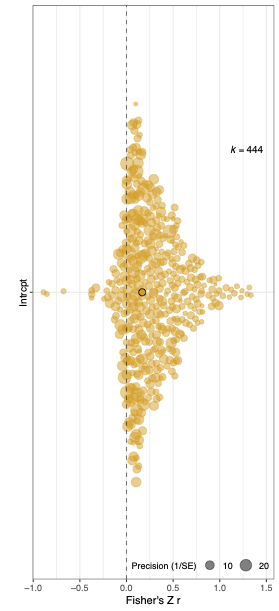
\includegraphics{ranksuccess_Fig1_orchard.png} \textbf{Figure 1.}
Orchard plot displaying the spread of the 444 effect sizes in our sample
(each dot represents a single effect size, the size of the dot indicates
the precision). Overall, most studies report a positive association
between dominance rank and reproductive success (darker circle in the
center indicates the mean). Our sample does show bias, with effect sizes
not distributed symmetrical around the center but showing an
overrepresentation of highly positive values.

\begin{center}\rule{0.5\linewidth}{0.5pt}\end{center}

~

There are potentially (at least) three sources of sample bias, the first
being `publication bias' with studies with low effect sizes (not
reaching traditional levels of significance) not ending up in the
published literature, the second being `study system bias' with research
focusing on populations with small groups where it is easy to detect
effects (e.g.~cooperative breeders), and the third being `study time
bias' with studies performed over shorter time frames generally being
more imprecise. We added further post-hoc analyses to investigate these
patterns individually here, and in combined models after identifying
which study systems might show different effect sizes (section R5.1).

Simple tests for `publication bias' (Preston, Ashby, and Smyth (2004))
suggest that effect sizes with a p-value smaller than 0.05 are about
four times more likely to be reported than effect sizes with a p-value
larger than 0.50.

As a further indication of `publication bias,' we find that studies with
small sample sizes and small effect sizes (those that presumably did not
reach statistical significance) are missing in our dataset such that the
average effect sizes at smaller sample sizes are more extreme than those
at larger sample sizes (estimate of sample size on effect sizes metafor
-0.03 - -0.02, rethinking -0.09 - -0.04) (Figure 2). Nevertheless, the
estimated effect sizes in this model remain consistently larger than
zero, indicating that even after including any missing studies with
small or negative effect sizes there would still be on average a
positive relationship between dominance rank and female reproductive
success across studies.

~

\begin{center}\rule{0.5\linewidth}{0.5pt}\end{center}

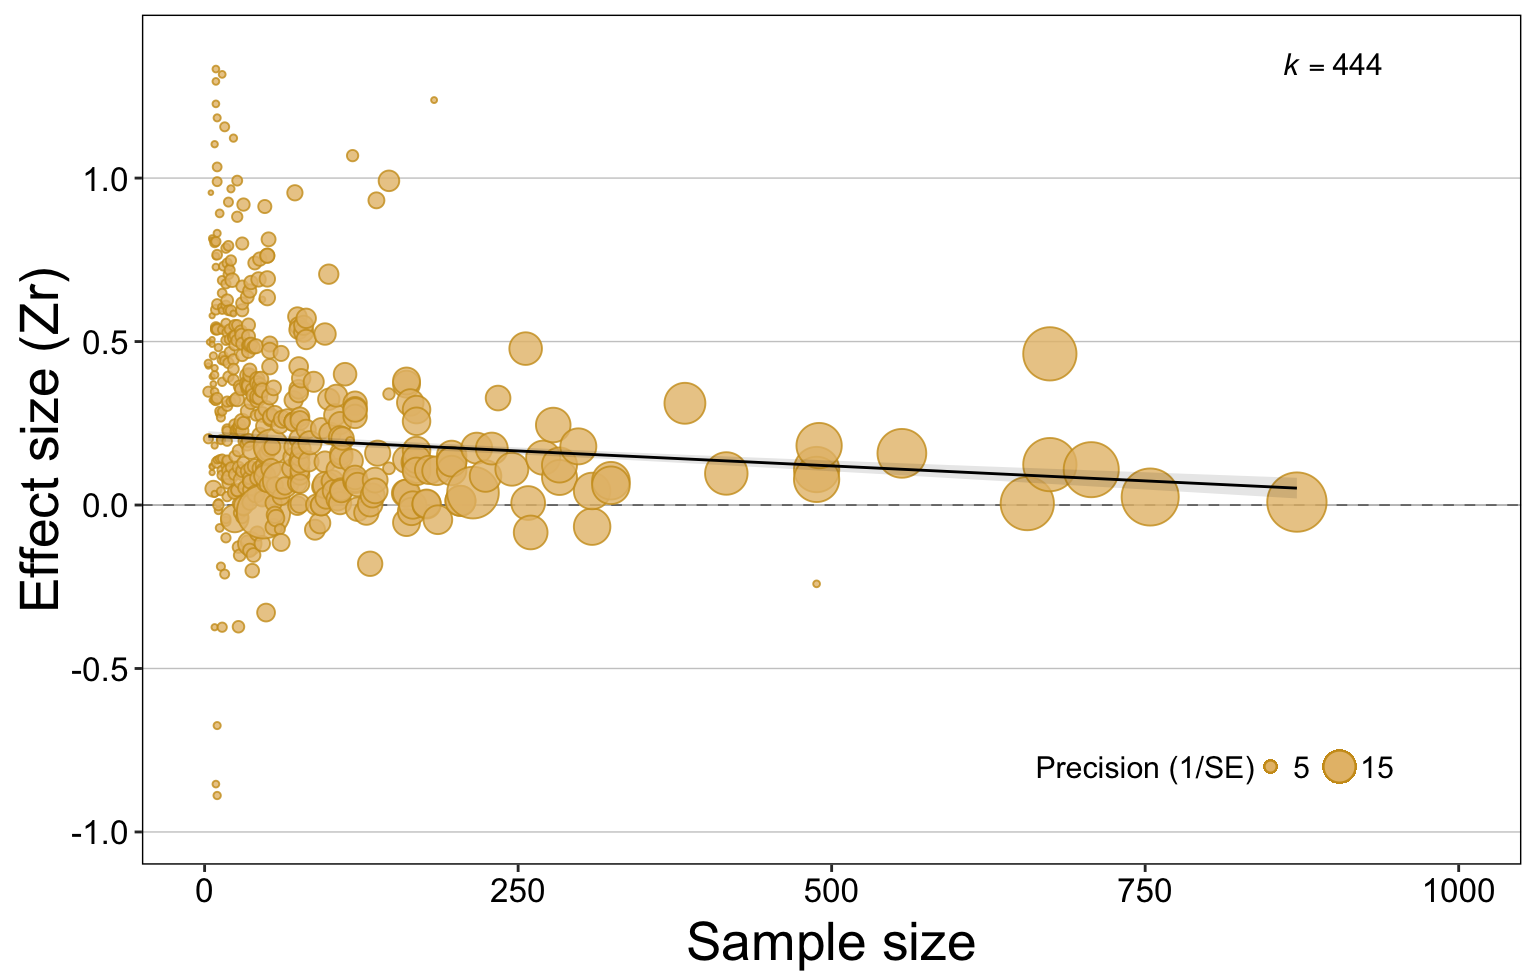
\includegraphics{ranksuccess_Fig2_effectsize_samplesize.png}

\textbf{Figure 2.} Relationship between the measured size of the effect
of dominance rank on female reproductive success and the sample size of
the study. Studies with smaller sample sizes show more extreme effect
sizes, and also indications of potential publication bias as there are
more extremely positive values than what would be expected based on the
average effect sizes of studies with larger sample sizes.

\begin{center}\rule{0.5\linewidth}{0.5pt}\end{center}

~

Our data also shows indication that the sample bias might result from
`study system bias,' because these base analyses indicate high
heterogeneity in our sample (total heterogeneity / total variability:
73.37\%). Given the diversity of studies in our sample, we did not
expect that the effect sizes represent a sample from a single
distribution: for example, studies of offspring mortality tend to have
larger sample sizes (because each mother can have multiple offspring)
and we predict different effect sizes for these studies. Sections R2 -
R4 present the specific analyses for each prediction to assess each of
the factors potentially leading to differences between effect size
estimates, and we combine them in section R5.1.

~

Finally, including the number of years a study had been conducted for as
a predictor of the effect sizes also indicates that our sample shows
`study time bias.' Effect sizes are lower when studies have been
conducted for longer (metafor estimate -0.01 - 0.00, rethinking estimate
-0.05 - 0.00), but in particular the variance is reduced once a study
has been running for 10 ore more years (Figure 3).

\begin{center}\rule{0.5\linewidth}{0.5pt}\end{center}

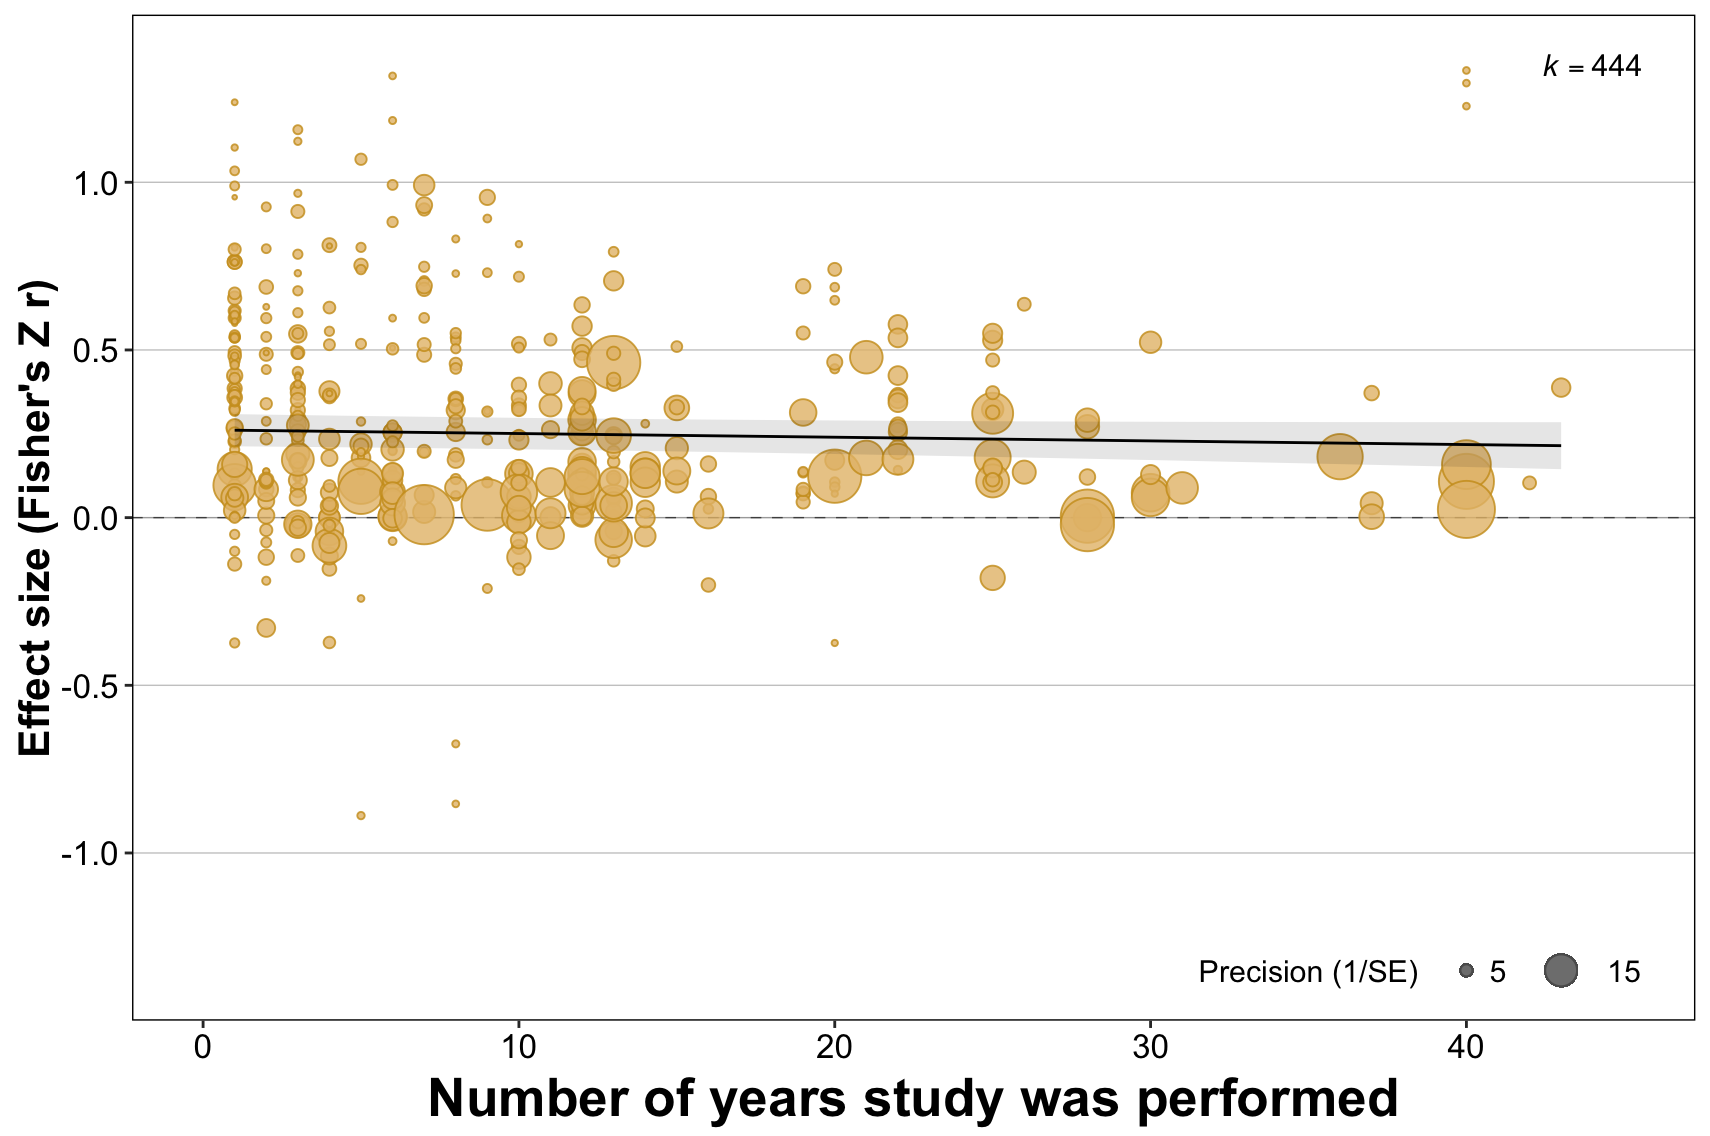
\includegraphics{ranksuccess_Fig3_effectsize_noyears.png} \textbf{Figure
3.} Relationship between the measured size of the effect of dominance
rank on female reproductive success and the length a study was conducted
for. Studies that have been conducted for 10 or more years tend to have
higher precision (larger circle) and tend to be closer to the overall
mean.

\begin{center}\rule{0.5\linewidth}{0.5pt}\end{center}

~

\textbf{R1.2 Overall effect}: We constructed an intercept-only
meta-analytic base model to test for a general effect of dominance rank
on reproductive success. Across our sample, there is a strong effect
that females with higher dominance rank have higher reproductive success
(metafor estimate +0.22 - +0.27, rethinking estimate +0.26 - +0.30; the
metafor estimate here and in the additional models is lower than the
rethinking estimate because the statistical approach of the former
expects the data to be more symmetrical than they are). This overall
effect means, for example, that in groups with two individuals dominants
would have between 0-6 offspring while subordinates have between 0-4
offspring. There is large variation though in our sample, with effect
sizes ranging from -0.89 - +1.33 (Figure 1).

~

\textbf{R1.3 Influence of locality/species}: To the base model, we added
random effects to account for non-independence due to effect sizes
originating from within the same study, from studies performed on the
same population and on the same species. The estimate of the overall
effect size did not change in this model (metafor estimate +0.22 -
+0.31, rethinking estimate +0.26 - +0.35). Effect sizes from the same
species and the same study, but not the same population, tend to be
similar to each other. The absence of a population effect could be
because there are only very few observations in our dataset of the same
population taken in different studies where there are also observations
from multiple additional populations of the same species. Alternatively,
it could be that effects do not vary across populations of the same
species, which is also indicated by the absence of differences between
wild and captive populations (see below).

~

\textbf{R1.4 Influence of phylogeny}: To the random effects model, we
added a covariance structure to reflect potential similarities in effect
sizes arising from closely related species showing similar effects due
to their shared phylogenetic history. Both statistical approaches
indicate that closely related species tend to have effect sizes that are
more similar than those of distantly related species. The metafor
approach suggests that about 20\% of the variation in effect sizes is
associated with covariation among species. The rethinking approach shows
high uncertainty in the estimates (Figure 4), reflecting the high
heterogeneity in the underlying data with high variation within species
and different measures taken among closely related species. It suggests
that species of the same genus tend to have similar effect sizes and
that shared phylogenetic history might also explain similarities in
effect sizes among species in the same Order, but covariance estimates
are close to zero for species pairs that are more distantly related
(Figure 4; the hightest standardized distance between any pair of
species in the same Order is 0.40).

\begin{center}\rule{0.5\linewidth}{0.5pt}\end{center}

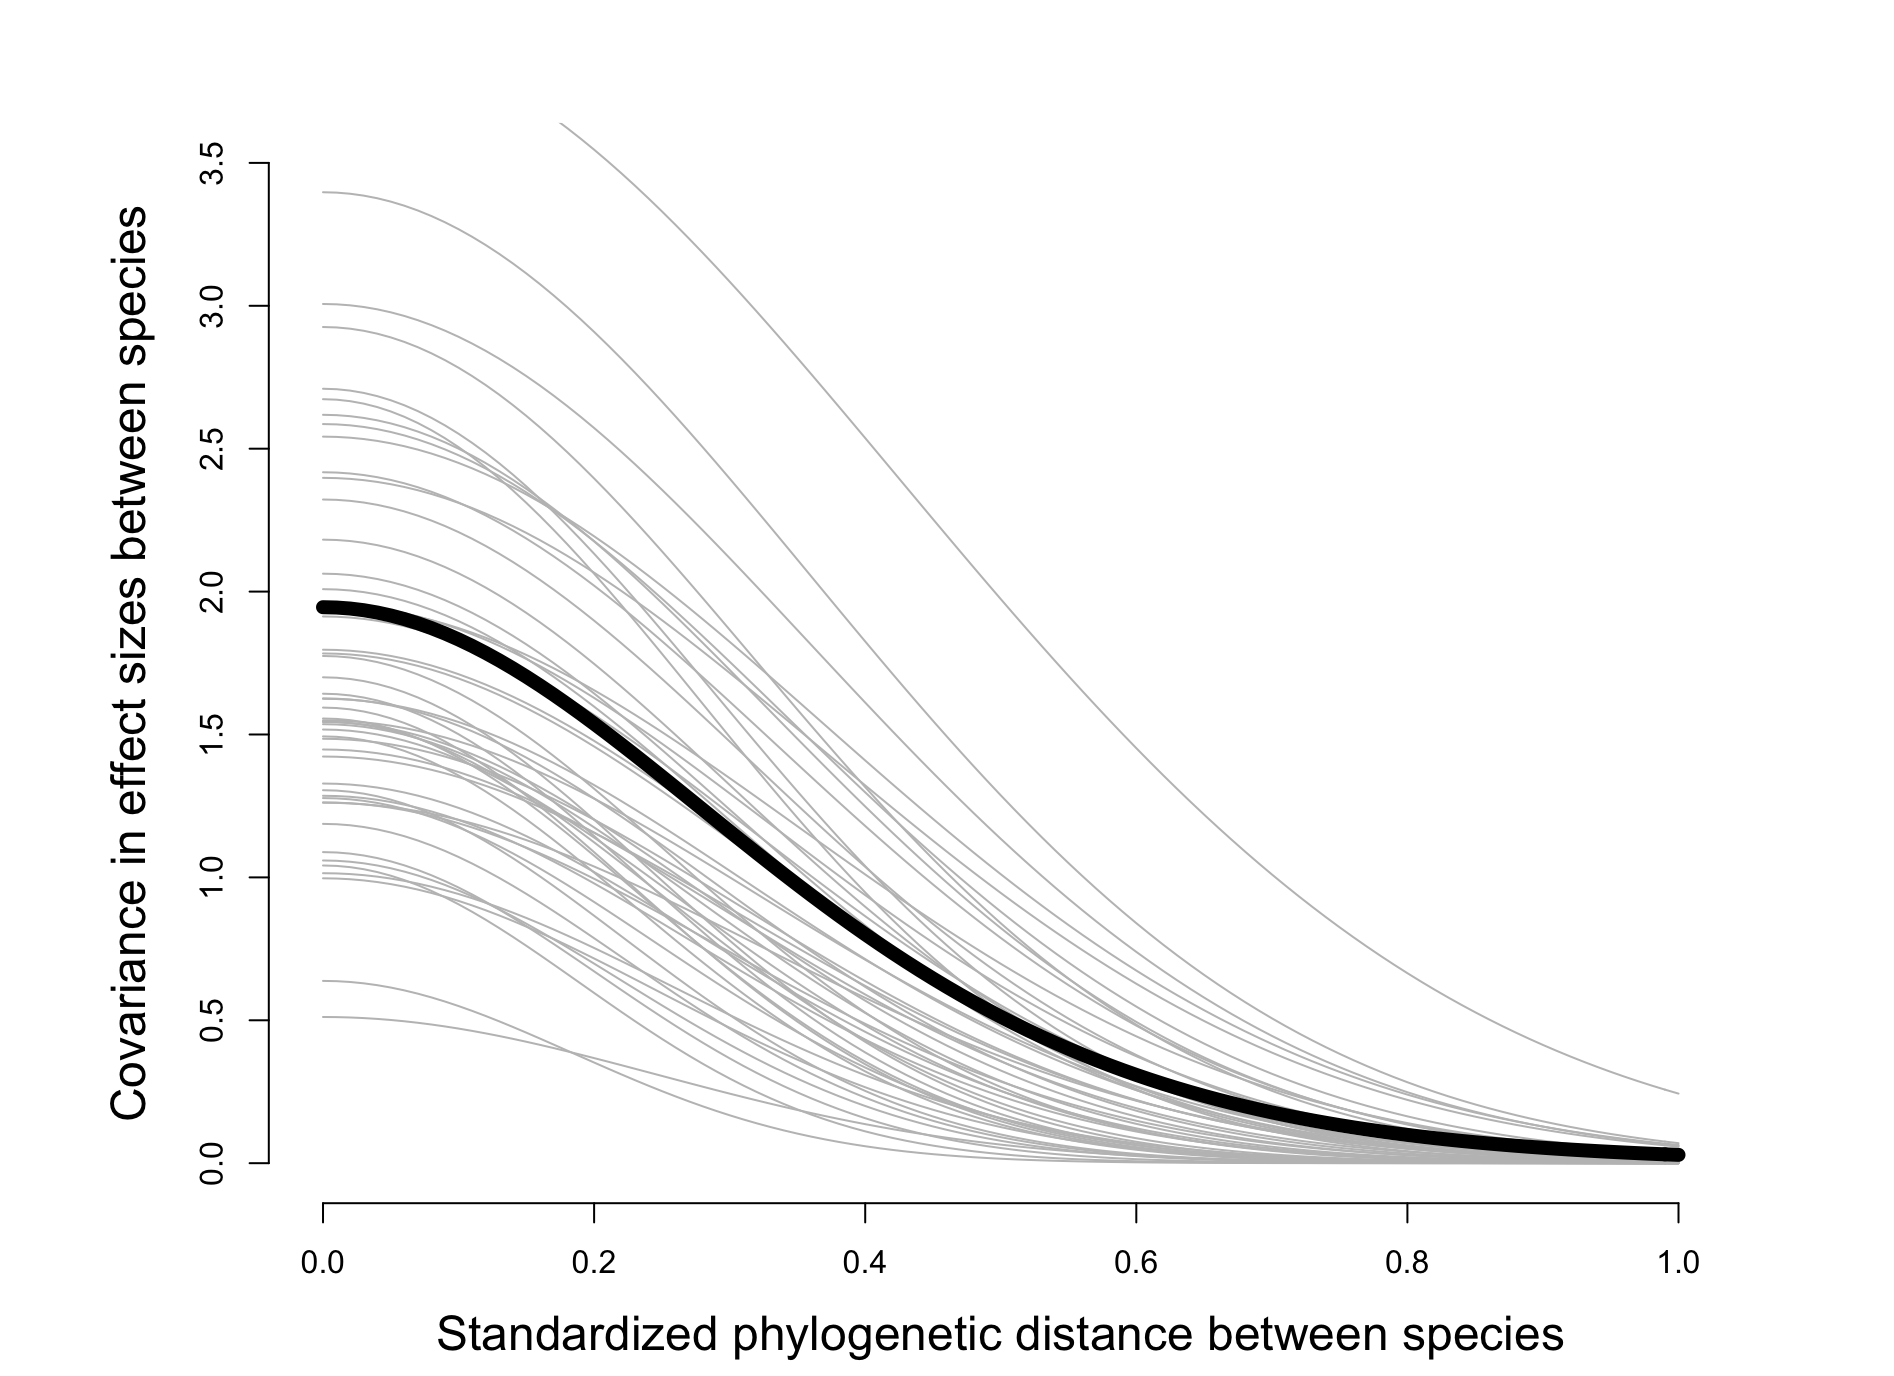
\includegraphics{ranksuccess_Fig4_covariation_phylogeny.png}
\textbf{Figure 4.} Relationship between the phylogenetic distance
between pairs of species and the similarity of their effect sizes (solid
black line represents mean estimate of rethinking model, grey lines
represent variation in the estimate). Species that are closely related
and share most of their phylogenetic history (standardized phylogenetic
distance close to zero) show intermediate levels of covariance in their
effect sizes of dominance rank on female reproductive success. The
covariance drops to low values at a standardized phylogenetic distance
of around 0.4, the level separating species that are part of the same
Order.

\begin{center}\rule{0.5\linewidth}{0.5pt}\end{center}

~

\textbf{R1.5 Influence of approach}: To the base model, we add random
effects reflecting the differences in approaches across studies
(dominance ranks classified continuous/categorical; dominance determined
through agonism/correlate; population type wild/provisioned/captive;
number of years of the study).

Studies which measured dominance rank categorically by classifying
individuals as either dominants or subordinates report higher effect
sizes (metafor estimate +0.29 - +0.35, rethinking estimate +0.31 -
+0.41; n=251 effect sizes) than studies assigning individuals continuous
ranks (metafor estimate 0.16-0.22, rethinking estimate +0.17 - +0.28;
n=193 effect sizes). In essentially all studies of cooperative breeders
(31 of 32 effect sizes), comparisons were between the single dominant
female and a class of the remaining subordinate females, which may
contribute to higher effect sizes for studies using categorical measures
of rank (see section R5.2.1).

Studies which determined the rank of females based on agonistic
interactions have lower effect sizes (metafor estimate +0.22 - +0.26,
rethinking estimate +0.24 - +0.32; n=407 effect sizes) than studies
which used other correlates (body size, age, etc.) to assign dominance
ranks (metafor estimate 0.43-0.55, rethinking estimate +0.41 - +0.63;
n=37 effect sizes). These 37 effect sizes where rank was assigned based
on correlates are from cooperative breeders and/or studies in which
groups consisted of mothers and their daughters.

Effect sizes did not vary between studies conducted with captive
(metafor estimate +0.24 - +0.30, rethinking estimate +0.27 - +0.37;
n=183 effect sizes), provisioned (metafor estimate +0.21 - +0.33,
rethinking estimate +0.14 - +0.41; n=23 effect sizes), or wild (metafor
estimate +0.22 - +0.34; n=283 effect sizes) individuals, and this does
not change when we nest the population type within species (indicating
that effect sizes do not differ between captive, provisioned, and wild
populations of the same species).

~

\hypertarget{what-are-the-life-history-traits-that-mediate-the-benefits-of-rank-on-reproductive-success-2}{%
\paragraph{\texorpdfstring{\textbf{2) What are the life history traits
that mediate the benefits of rank on reproductive
success?}}{2) What are the life history traits that mediate the benefits of rank on reproductive success?}}\label{what-are-the-life-history-traits-that-mediate-the-benefits-of-rank-on-reproductive-success-2}}

~

\textbf{R2.1 Influence of measure of reproductive success}: To the base
model, we add a predictor variable reflecting the six classes of
measures of reproductive success.

Dominance rank appears to have the highest effect on age at first
conception (metafor estimate +0.32 - +0.43, rethinking estimate +0.33 -
+0.52; n=23 effect sizes), life time reproductive success (metafor
estimate +0.27 - +0.40, rethinking estimate +0.31 - +0.47; n=34 effect
sizes), interbirth interval (metafor estimate +0.25 - +0.37, rethinking
estimate +0.28 - +0.37; n=46 effect sizes), infant production (metafor
estimate +0.21 - +0.33, rethinking estimate +0.23 - +0.38; n=198 effect
sizes), adult survival (metafor estimate +0.18 - +0.31, rethinking
estimate +0.18 - +0.34; n=30 effect sizes), infant survival (metafor
estimate +0.14 - +0.25, rethinking estimate +0.15 - +0.26; n=113 effect
sizes). Effects of dominance rank on survival are lower than on other
measures of female fitness. In addition, females themselves appear to
benefit more than their offspring (adult survival \textgreater{} infant
survival). While effect sizes for life time reproductive success are
higher than those for the values from which it is usually calculated
(adult survival, interbirth interval, infant production), there does not
appear to be a straightforward additive (or multiplicative) combination
of the individual effects (Figure 5)

\begin{center}\rule{0.5\linewidth}{0.5pt}\end{center}

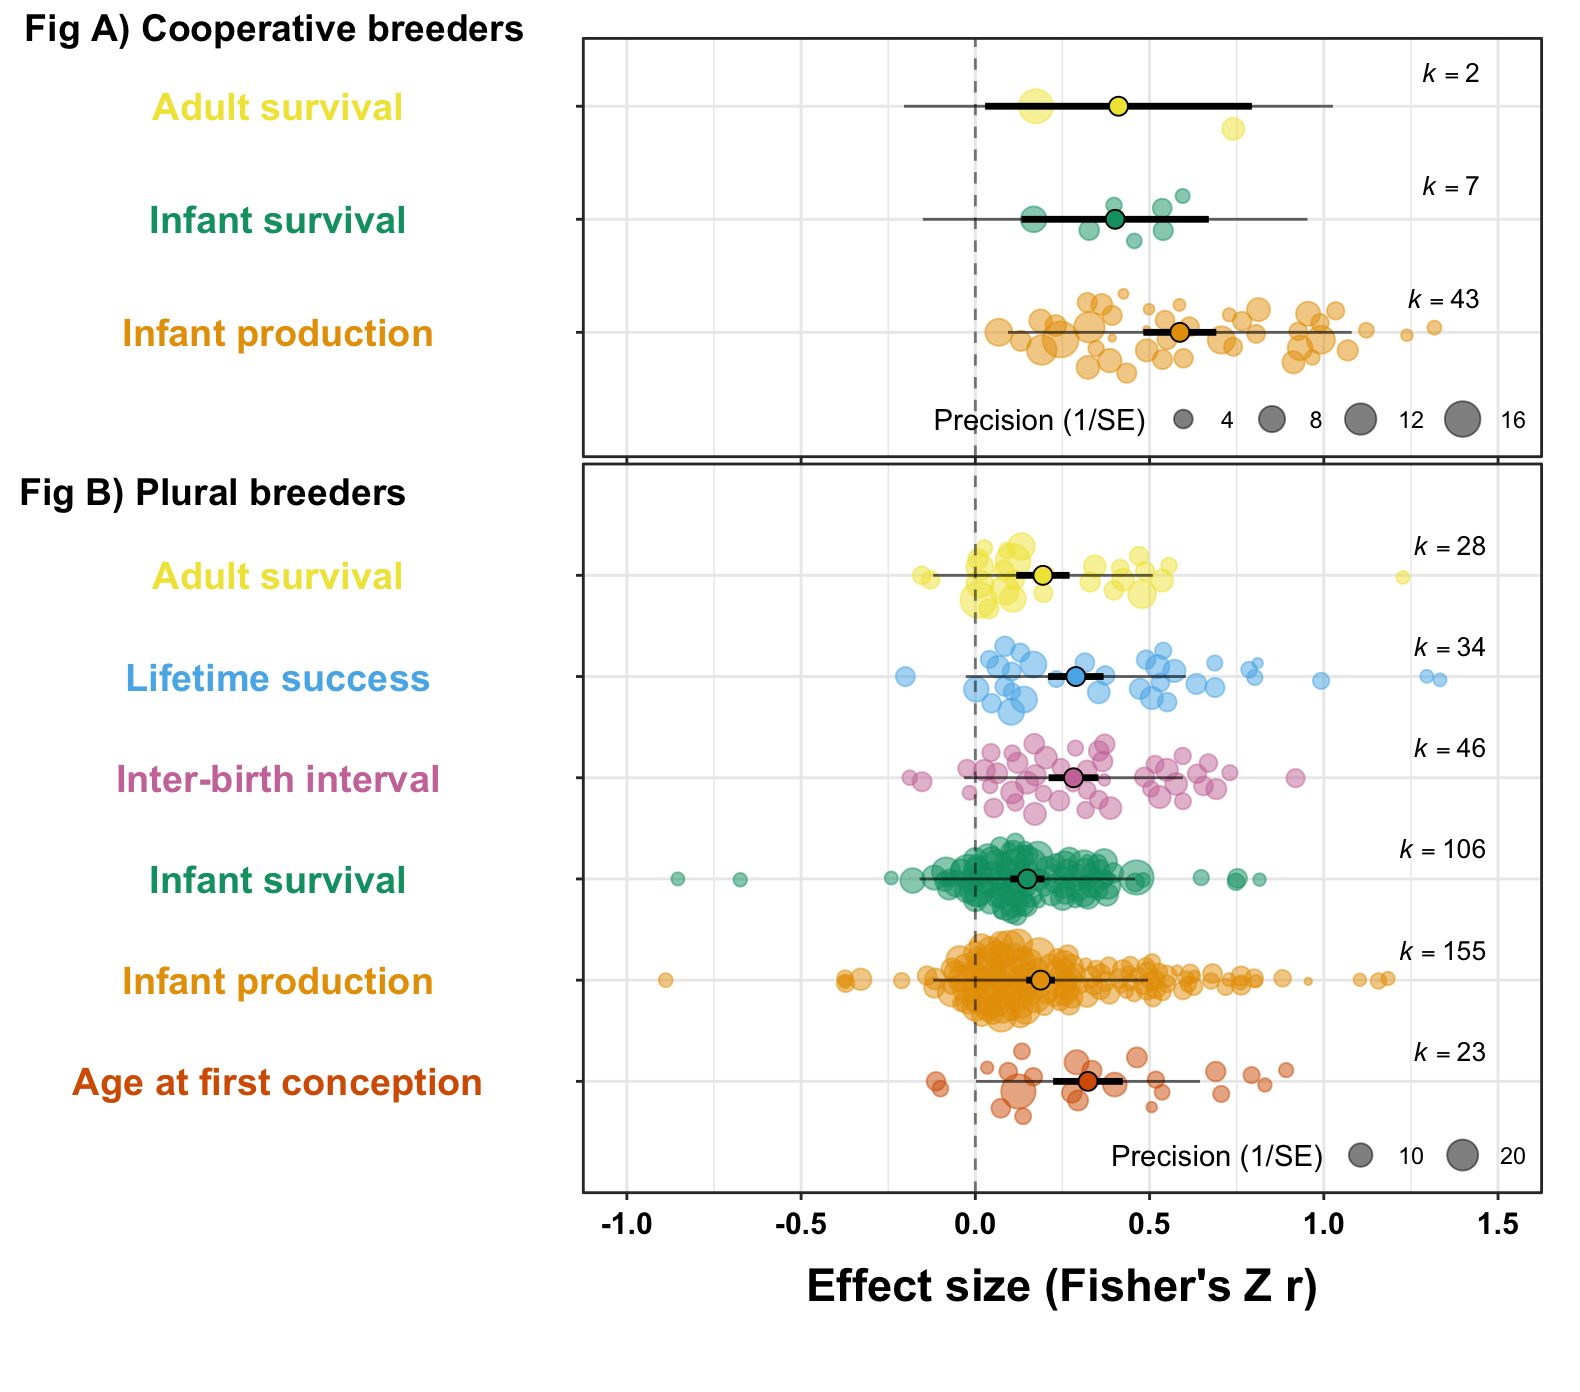
\includegraphics{ranksuccess_Fig5_effectsize_lifehistorymeasure.png}
\textbf{Figure 5.} Raw effect sizes of dominance rank on reproductive
success are generally higher for cooperative breeders (a) than for
plural breeders (b), and differ according to the measure of reproductive
success. In general, dominance appears to have stronger effects on
reproductive output (lifetime reproductive success, age at first
conception, infant production, inter-birth intervals) than on survival
(both of the adult females themselves and of their infants). The
differences between measures of reproductive success change slightly
when accounting for similarity among observations from the same and
related species, but the ordering remains the same.

\begin{center}\rule{0.5\linewidth}{0.5pt}\end{center}

~

\textbf{R2.2 Litter Size and Litters Per Year} Effects of dominance on
reproductive success are higher in species with larger litter sizes
(metafor estimate of litter size +0.03 - +0.05, rethinking estimate
+0.05 - +0.09; n=444 effect sizes) and with more litters per year
(metafor estimate of litters per year +0.04 - +0.08, rethinking estimate
+0.06 - +0.11; n=444 effect sizes). Effect sizes in species where
females produce single offspring are on average 0.25 while effect sizes
in species where females produce litters are on average 0.34, and effect
sizes in species where females produce one or fewer litters per year are
on average 0.25 while effect sizes in species where females produce
multiple litters each year are on average 0.45. The association of the
effect sizes with the number of litters per year remained when
accounting for the phylogenetic relatedness among species, but the
association with litter size did not, suggesting that it might be
influenced by other characteristics that differ among species with
variable litter sizes.

~

\hypertarget{what-are-the-ecological-conditions-that-mediate-the-benefits-of-rank-on-reproductive-success-2}{%
\paragraph{\texorpdfstring{\textbf{3) What are the ecological conditions
that mediate the benefits of rank on reproductive
success?}}{3) What are the ecological conditions that mediate the benefits of rank on reproductive success?}}\label{what-are-the-ecological-conditions-that-mediate-the-benefits-of-rank-on-reproductive-success-2}}

~

\textbf{R3.1 Diet Category}

Effect sizes are larger in carnivores (0.36; n=72 effect sizes) than in
omnivores (0.29; n=227 effect sizes), herbivores (0.27; n=117 effect
sizes), or frugivores (0.22; n=28 effect sizes) (estimated difference
carnivores versus omnivores metafor -0.36 - -0.17 rethinking -0.24 -
-0.04, difference carnivores versus herbivores metafor -0.29 - -0.13
rethinking -0.16 - -0.03, difference carnivores versus frugivores
metafor -0.27 - -0.11 rethinking -0.14 - -0.02; estimates for all other
comparisons cross 0). Carnivores are no longer estimated to have
different effect sizes when the phylogenetic relatedness among species
is taken into account, potentially due to the higher prevalence of
cooperative breeding in carnivores.

~

\textbf{R3.2 Environmental Harshness}

Our data shows no association between environmental harshness and the
effect of dominance rank on reproductive success (metafor estimate -0.3
- +0.4, rethinking -0.6 - +0.1; no change when accounting for shared
phylogenetic history; n=259 effect sizes).

~

\textbf{R3.3 Population Density}

Effect sizes are larger in species with higher population densities
(metafor +0.04 - +0.08, rethinking +0.05 - +0.10; n=346 effect sizes),
even when including phylogenetic relatedness.

~

\hypertarget{what-are-the-social-circumstances-that-mediate-the-benefits-of-rank-2}{%
\paragraph{\texorpdfstring{\textbf{4) What are the social circumstances
that mediate the benefits of
rank?}}{4) What are the social circumstances that mediate the benefits of rank?}}\label{what-are-the-social-circumstances-that-mediate-the-benefits-of-rank-2}}

~

\textbf{R4.1 Breeding system}

Effect sizes of cooperative breeders (average 0.58; n=52 effect sizes)
are higher than those observed in plural (average 0.25; n=324 effect
sizes) or associated breeders (average 0.23; n=68 effect sizes)
(estimates for difference cooperative breeder vs plural breeder metafor
-0.40 - -0.30, rethinking -0.41 - -0.27; cooperative breeder vs
associated breeder metafor -0.47 - -0.35, rethinking -0.45 - -0.26;
plural breeder vs associated breeder metafor -0.07 - +0.05, rethinking
-0.07 - +0.05). Cooperative breeders are still estimated to have higher
effect sizes than species with other breeding systems when accounting
for phylogenetic relatedness, but the differences are slightly reduced
(Figure 5).

~

\textbf{R4.2 Dominance System}

Effect sizes are higher in species in which condition plays a major role
in determining which females are dominant rather than subordinate
(average effect size 0.38; n=94 effect sizes), compared to species in
which age (average effect size 0.31; n=100 effect sizes) or nepotism
(average effect size 0.24; n=243 effect sizes) influence dominance rank
(estimates for difference condition vs age: metafor +0.05 - +0.17,
rethinking +0.01 - +0.16; condition vs nepotism: metafor +0.07 - +0.20,
rethinking +0.08 - +0.20; age vs nepotism: metafor -0.07 - +0.03,
rethinking -0.01 - +0.12). Species with different dominance system are
no longer estimated to be different when including the phylogenetic
similarity.

We had initially planned to assess whether dominance effect appear
across different time scales depending on how dominant females acquire
their position. However, this turned out to be more difficult. The
species in our dataset have vastly varying lifespans, so simply
assessing the number of years a study had been conducted for skews the
observation towards short-lived species. The values for the relative
duration (number of years studied divided by the maximum lifespan of the
species) show that 90\% of effect sizes are from studies that lasted
less than 10\% of the lifespan of the species (median 3\%). In all of
the 19 species in which studies spanned more than 10\% of the lifespan,
females acquire rank by nepotism. We did not find any consistent pattern
of relationship between effect size and study duration dependent on the
system of dominance acquisition.

~

\textbf{R4.3 Philopatry}

The effects of dominance rank on reproductive success are higher in
species in which females disperse and join new groups (average effect
size 0.46; n=55 effect sizes) compared to species in which most females
were born in the same group they breed (average effect size 0.26; n=360
effect sizes) (metafor estimate of difference -0.24 - -0.12, rethinking
estimate -0.25 - -0.11), also when accounting for phylogenetic
covariance (Figure 6).

\begin{center}\rule{0.5\linewidth}{0.5pt}\end{center}

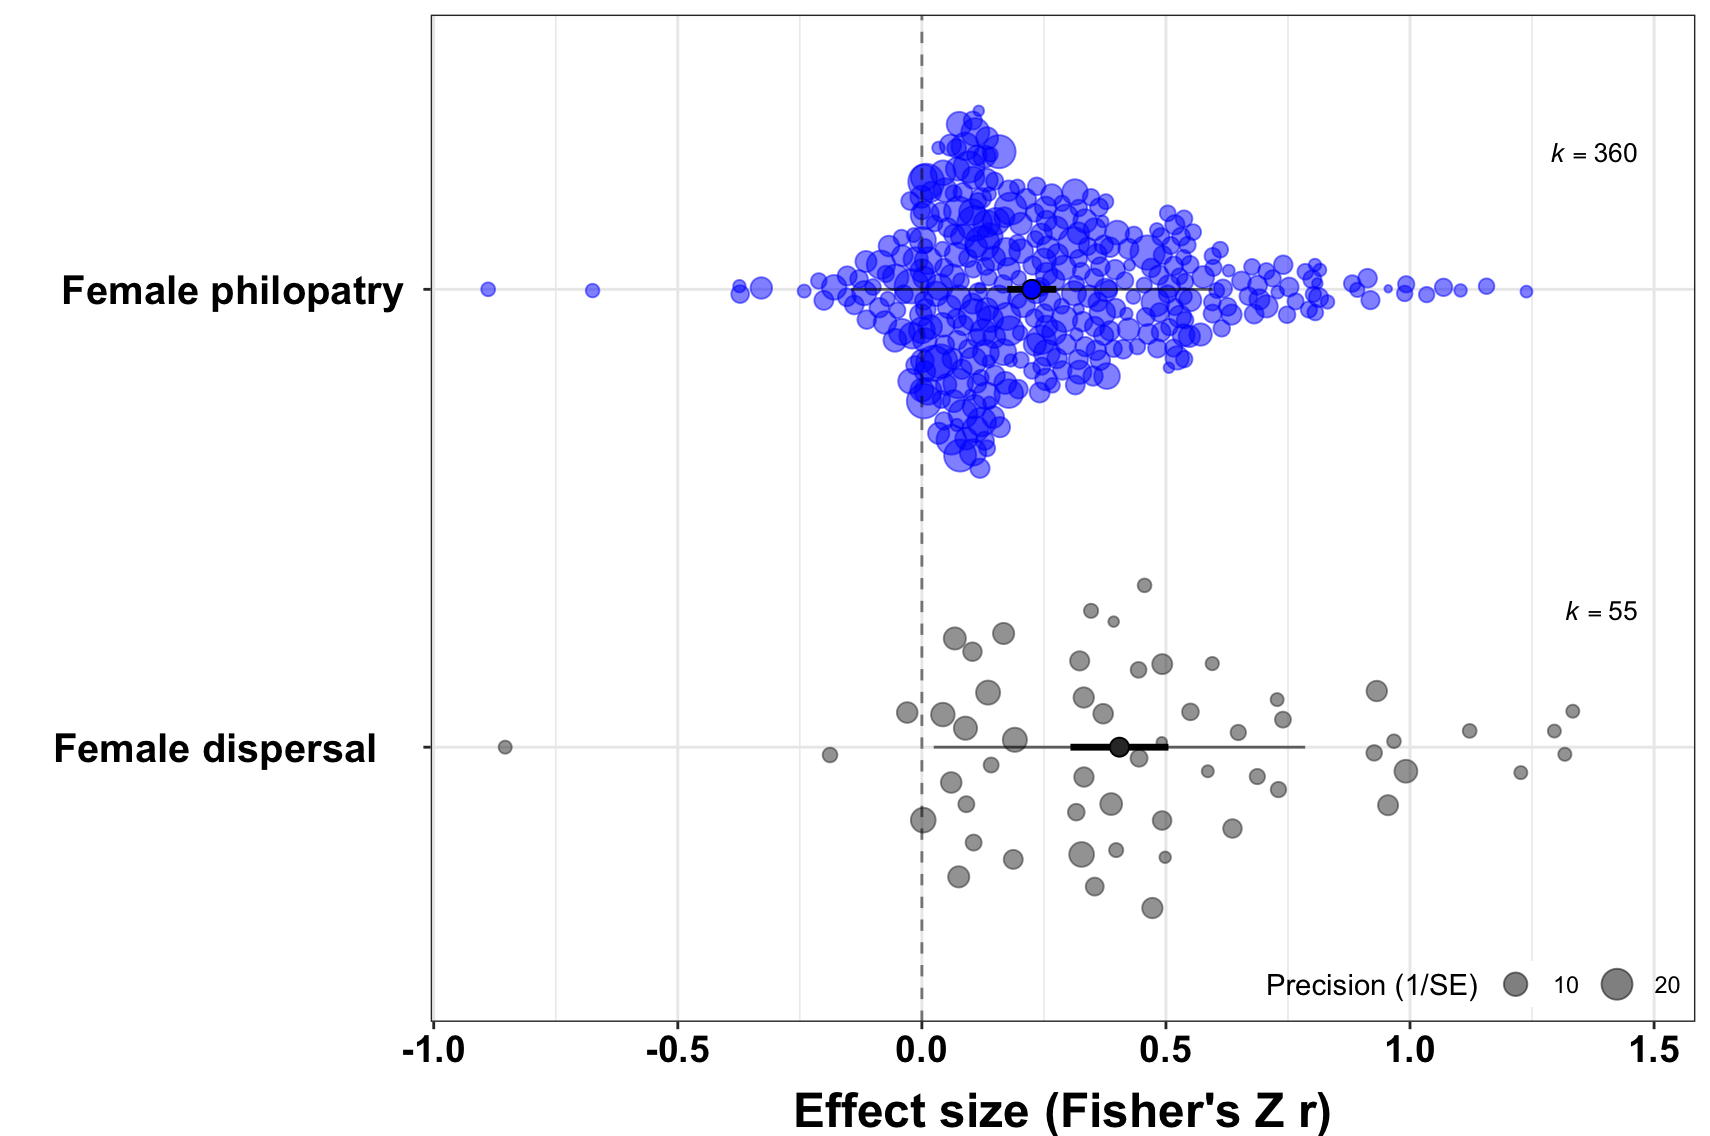
\includegraphics{ranksuccess_Fig6_effectsize_philopatry.png}
\textbf{Figure 6.} Effect sizes of dominance rank on female reproductive
success are lower in species in which which females are philopatric and
remain in the group/area where they have been born (top, blue dots) than
in species in which females disperse to breed (bottom, grey dots).

\begin{center}\rule{0.5\linewidth}{0.5pt}\end{center}

~

\textbf{R4.4 Group size}

Both approaches detect a negative association between the effect sizes
and group sizes (metafor estimate of log group size -0.099 - -0.678,
rethinking estimate of standardized group size -0.10 - -0.05; n=444
effect sizes). Compared to groups of 2 females, groups of 10 females
show \textasciitilde10\% lower effect sizes and groups of
\textasciitilde50 females show 50\% lower effect sizes. The negative
association between group size and the effect sizes remains when
accounting for similarity among closely related species.

~

\textbf{R4.5 Average Relatedness}

Effect sizes of dominance rank on reproductive success increase with
increasing levels of average relatedness among female group members
(metafor estimate +0.31 - +0.59, rethinking estimate +0.31 - +0.71;
n=288 effect sizes), though the association is no longer detected when
including the shared phylogenetic history among species (metafor
estimate -0.01 - +0.56; rethinking estimate -0.02 - +0.65).

~

\textbf{R4.6 Variance in relatedness}

We could not assess this prediction because sufficient data was not
available.

~

\textbf{R4.7 Coalition formation}

Species in which females form coalitions show only slightly lower
effects of dominance rank on reproductive success (average 0.27; n=246
effect sizes) than species in which females do not have support during
aggressive interactions (average 0.32; n=180 effect sizes) (estimate of
difference metafor: -0.11 - -0.01, rethinking -0.09 - +0.01), with no
difference in models accounting for similarity due to phylogenetic
relatedness (metafor -0.10 - +0.07; rethinking -0.09 - +0.03).

~

\textbf{R4.8 Intersexual conflict}

Effect sizes are larger in species in which sex ratios in social groups
are more balanced and lower when there are fewer males per female
(metafor estimate +0.55 - +1.25, rethinking estimate +0.07 - +0.11;
n=328 effect sizes), and the association remains the same when
accounting for shared phylogenetic history.

Effect sizes are lower in species in which males commit infanticide
(metafor estimate -0.20 - 0.00; rethinking estimate -0.15 - -0.04; n=332
effect sizes), but the relationship does not hold when accounting for
phylogenetic relatedness (metafor -0.13 - +0.07, rethinking -0.07 -
+0.06).

Differences in effect sizes are not associated with the extent of sexual
dimorphism in body size across species (metafor estimate -0.17 - 0.11;
rethinking -0.05 - +0.01; similar estimates when accounting for sharerd
phylogenetic history; n=334 effect sizes).

\textbf{R4.9 Macaque dominance styles}

Differences in dominance styles among macaques are not associated with
the effect of dominance rank on reproductive success (metafor estimates
effect sizes of species in Grade 1 to be different from species in Grade
2 +0.05 - +0.12 but no differences for the five other pairwise Grade
comparisons; rethinking estimates for all comparisons overlap zero; n =
109 effect sizes from 9 species). Egalitarian species do not show lower
effects of dominance rank on reproductive success than other species and
the sample size is too small to determine whether despotic species
systematically differ from other species (Figure 7).

\begin{center}\rule{0.5\linewidth}{0.5pt}\end{center}

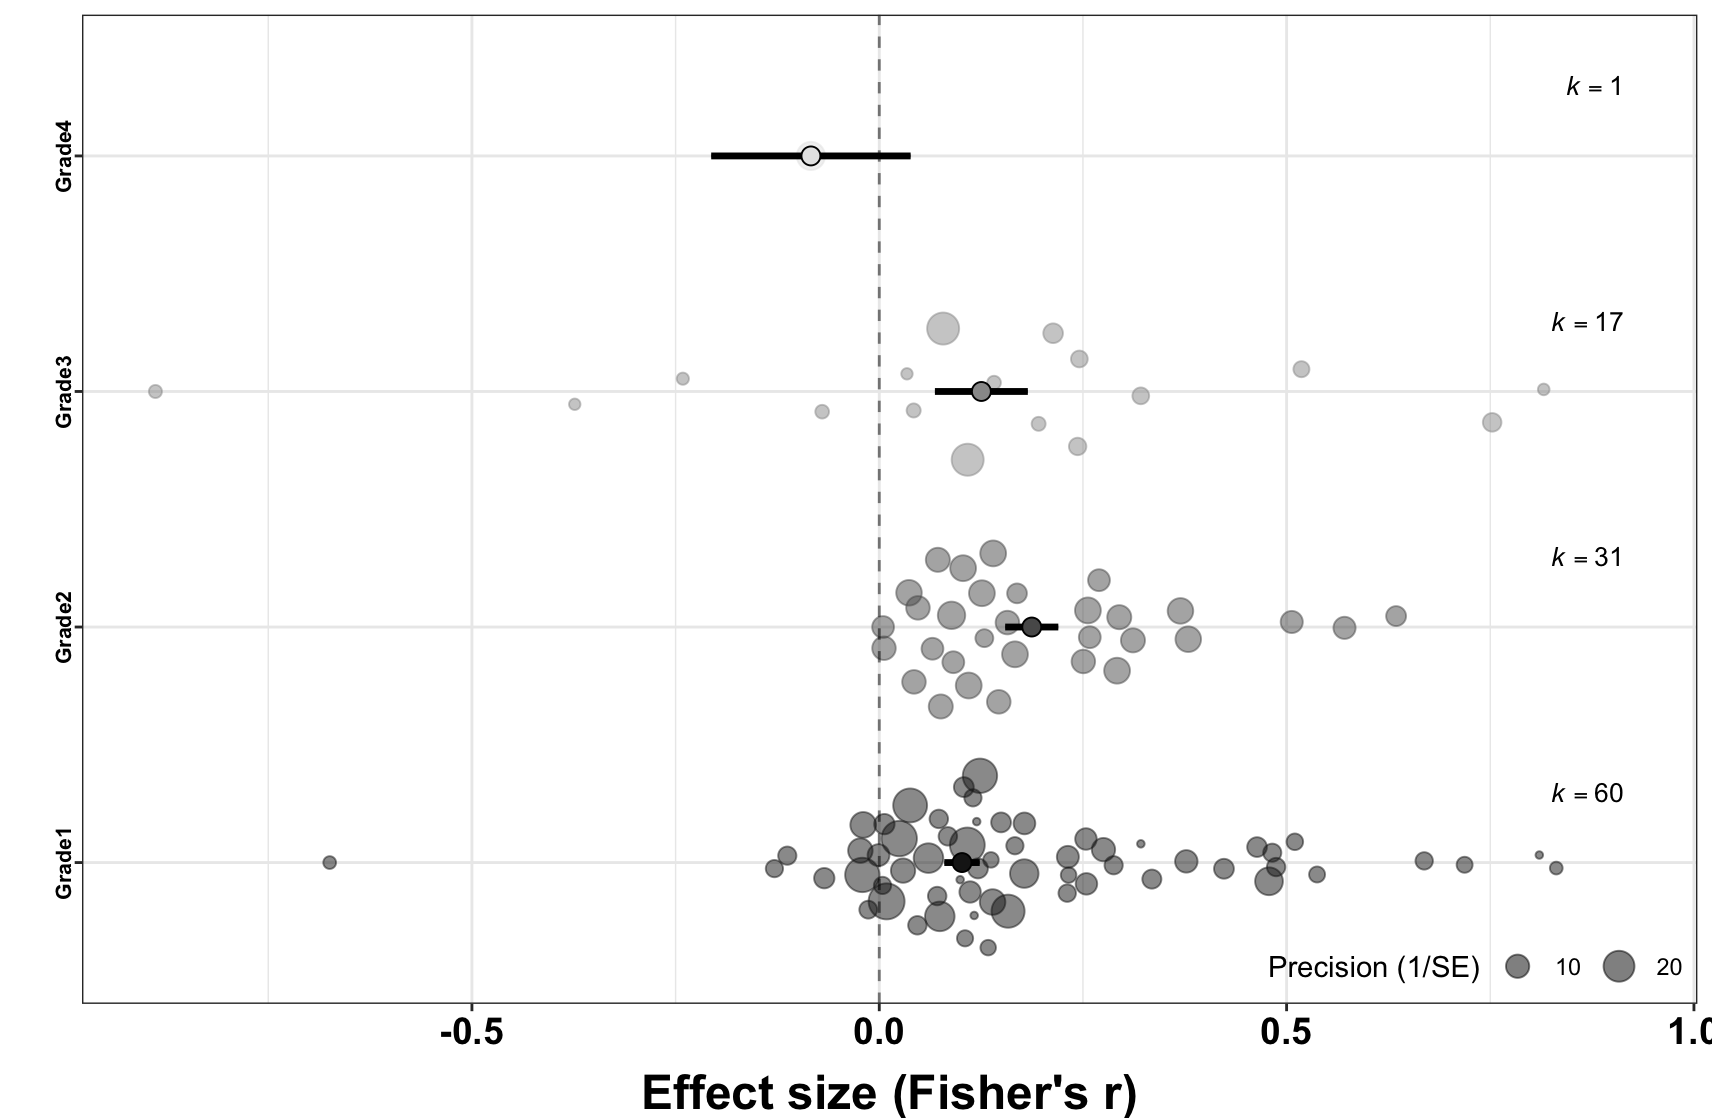
\includegraphics{ranksuccess_Fig9_effectsizes_macaquedominancestyles.png}
\textbf{Figure 7.} The effect of dominance rank on female reproductive
success is similar across macaque species with different dominance
styles. Relationships among female group members in species of grade 1
(bottom dark grey) are generally considered egalitarian, while grade 4
(top light grey) is assigned to species in which relationships are
deemed highly despotic. Species with different dominance styles are not
estimated to be different (all posterior contrasts overlap zero).

\begin{center}\rule{0.5\linewidth}{0.5pt}\end{center}

~

~

\hypertarget{summary-of-univariate-analyses}{%
\paragraph{\texorpdfstring{\textbf{Summary of univariate
analyses}}{Summary of univariate analyses}}\label{summary-of-univariate-analyses}}

\hfill\break
Overall, our data indicate that females of higher rank generally have
higher reproductive success than females of lower rank. In terms of the
approach, effect sizes of dominance rank on reproductive success were
higher (i) when individuals were assigned a rank category rather than a
continuous position, (ii) when rank was determined using indirect
measures rather than aggressive interactions, and (iii) in some studies,
species, and families of species than in others. We found no differences
in effect sizes when studies were conducted in a captive rather than a
wild setting. Effect sizes of dominance rank were higher for measures of
reproductive output than for measures of survival, and higher for
measures of maternal than offspring fitness.

We found that effect sizes of dominance rank on reproductive success are
associated with six of our single predictor variables, whereas we did
not find an association with another eight of the single predictor
variables (Table 1). Five of the six associated predictor variables
reflect variation in the social environment, while we did not find any
association with any of the predictor variables reflecting the
ecological environment.

\begin{center}\rule{0.5\linewidth}{0.5pt}\end{center}

\textbf{Table 1.} Overview of \textbf{variables associated with
variation in effect sizes of dominance rank on female reproductive
success} in univariate analyses. The following six variables (of the
fourteen we assessed) are estimated to explain variation in the effect
sizes with both approaches when accounting for shared phylogenetic
history among the species in our sample.

\begin{tabu} to \linewidth {>{\raggedright}X>{\raggedright}X>{\raggedright}X}
\hline
Predictor variable & Metafor compatibility estimate of association & Rethinking compatibility estimate of association\\
\hline
litters per year & +0.03 - +0.05 & +0.05 - +0.09\\
\hline
population density & +0.04 - +0.08 & +0.05 - +0.10\\
\hline
group size & -0.07 - -0.01 & -0.10 - -0.05\\
\hline
cooperative breeding & +0.30 - +0.40 & +0.27 - +0.41\\
\hline
philopatry & -0.24 - -0.12 & -0.25 - -0.11\\
\hline
sex ratio & +0.44 - +1.25 & +0.07 - +0.11\\
\hline
\end{tabu}

\textbf{Table 2.} Overview of \textbf{variables not associated with
variation in effect sizes of dominance rank on female reproductive
success} in univariate analyses. The following eight variables (of the
fourteen we assessed) are estimated to not be linked with variation in
the effect sizes when accounting for shared phylogenetic history among
the species in our sample.

\begin{tabu} to \linewidth {>{\raggedright}X>{\raggedright}X>{\raggedright}X}
\hline
Predictor variable & Metafor compatibility estimate of association & Rethinking compatibility estimate of association\\
\hline
litter size & -0.01 - +0.03 & -0.04 - +0.09\\
\hline
dominance acquisition & -0.07 - +0.03 & -0.01 - +0.12\\
\hline
diet & -0.04 - +0.03 & -0.10 - +0.06\\
\hline
environmental harshness & -0.30 - +0.40 & -0.60 - +0.10\\
\hline
average relatedness & -0.01 - +0.56 & -0.01 - +0.12\\
\hline
female coalitions & -0.10 - +0.07 & -0.09 - +0.07\\
\hline
male infanticide & -0.13 - +0.07 & -0.07 - +0.06\\
\hline
sexual dimorphism & -0.17 - +0.11 & -0.05 - +0.01\\
\hline
\end{tabu}

~

~

\hypertarget{combined-analyses}{%
\paragraph{\texorpdfstring{\textbf{5) Combined
analyses}}{5) Combined analyses}}\label{combined-analyses}}

~

\textbf{R5.1 Heterogeneity and sample bias}

The sample bias, namely the over-representation of extreme effect sizes,
in our data likely results from all three influences of (i) publication
bias, (ii) study system bias, and (iii) study time bias. In addition to
the direct indications of publication and study system bias in our
sample, our univariate analyses identified many factors that could lead
to study system bias. For example, while less than 5\% of all mammalian
species are cooperative breeders, 12\% of all effect sizes in our sample
come from cooperative breeders which have high positive effect sizes.

To identify the potential interplay between the three biases, we built
combined models. If biases occur because study systems with different
effect sizes also have particular sample sizes and study duration
(e.g.~cooperative breeders tend to live in smaller groups), we should no
longer detect an association between sample size and study duration with
the effect sizes when controlling for the different study systems. The
combined models indicate that the study system factors identified in the
uni-variate analyses are directly associated with variation in effect
sizes (all their estimates do not overlap zero), as is sample size, but
not the number of years a study had been conducted for. This indicates
that our sample has both publication and study system bias. The lack of
a direct influence of study time bias presumably occurs because sample
size is associated with the number of years a study has been conducted
for, indicating that large samples both in terms of time period or
breadth might reduce noise.

The reduction in publication bias when accounting for the study system
bias is visible when comparing the funnel plot of the raw effect sizes
in relation to their precision (Figure 8a), which shows a clear
asymmetry, to the funnel plot of the effect sizes adjusted for known
predictors (Figure 8b), which only indicates some large effect sizes at
small precision that are not balanced.

\begin{center}\rule{0.5\linewidth}{0.5pt}\end{center}

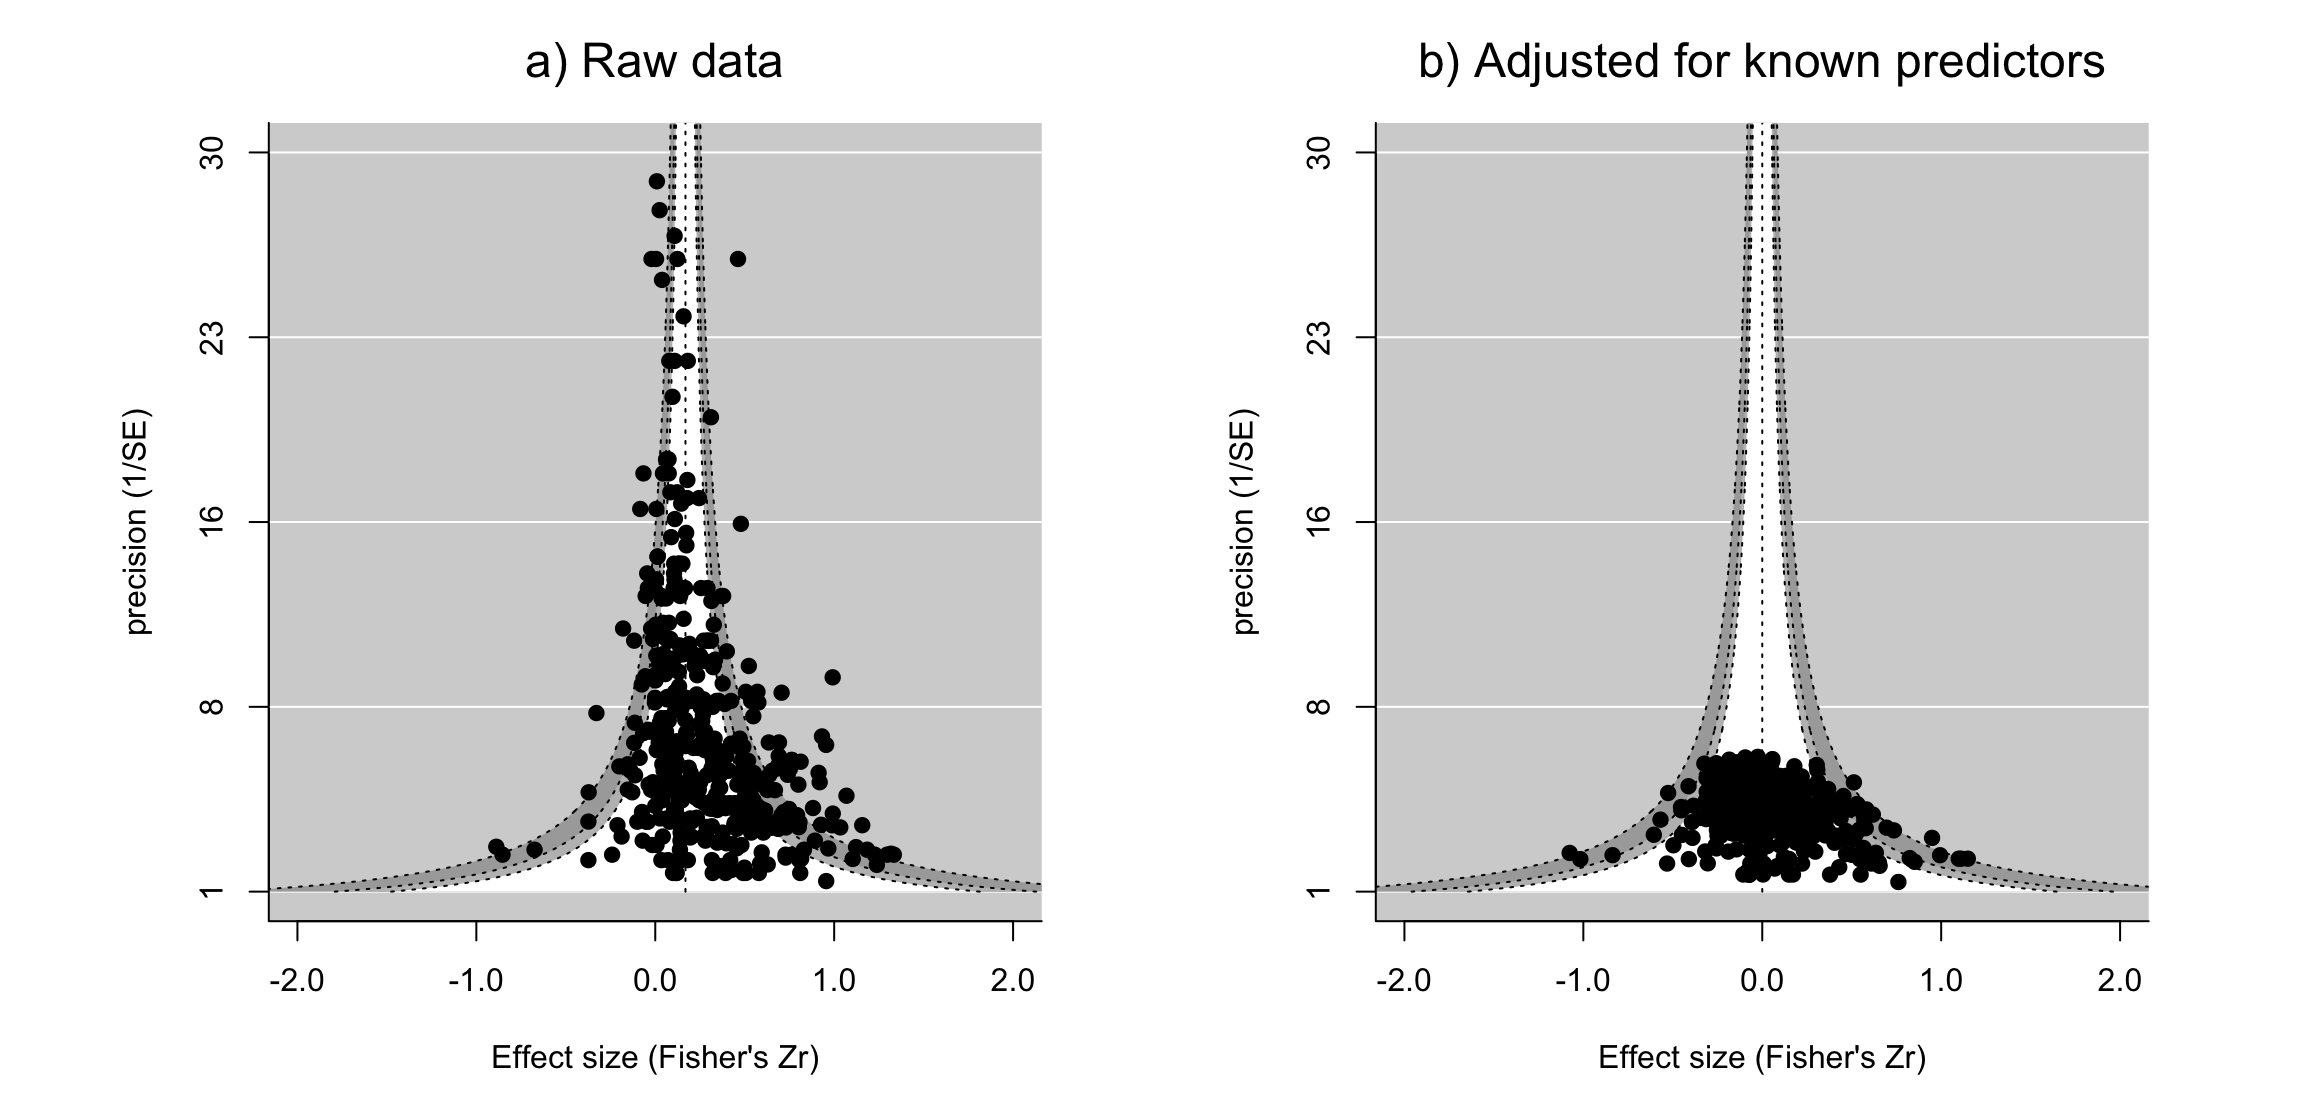
\includegraphics{ranksuccess_Fig7_effectsize_funnelplot.png}
\textbf{Figure 8.} Funnel plots based on raw effect sizes (a) and effect
sizes adjusted for known predictors (b). When accounting for the
influence of which reproductive trait was measured, whether the species
is a cooperative breeder or not, the number of litters per year the
species produces, and the phylogenetic covariance among species, the
distribution of the 444 effect sizes in our sample appears much less
imbalanced (b) than the raw effect sizes (a). The mean effect size (grey
dotted line in the center going upwards) is shifted close to zero when
adjusting for known predictors because these predictors explain why some
studies have positive effect sizes. Precision decreases for most
estimates because they no longer represent the measured values but the
values inferred from the interaction of the predictors.

\begin{center}\rule{0.5\linewidth}{0.5pt}\end{center}

~

\textbf{R5.2 Differences between cooperative and plural/associated
breeders}

In our preregistration, we had decided to first construct univariate
models as reported above, testing the influence of a single variable at
a time to assess support for the specific predictions. One of the main
factors that we found to be associated with higher effect sizes is
cooperative breeding. Cooperative breeders differ in many additional
aspects, so we first checked whether any of the other associations we
detect occur because they covary with cooperative breeding.

\textbf{R5.2.1 Differences in approach to study cooperative breeders}

Approaches of assigning rank depend on the breeding system of the study
species, with many studies of cooperative breeders assigning rank into
categories (98\% categorical, 2\% continuous) based on other measures
(50\% agonism, 50\% other) while studies of plural and associated
breeders often assign continuous ranks (51\% categorical, 49\%
continuous) based on agonistic interactions (97\% agonism, 3\% other).
Combining the variables representing the different study approaches with
the variable representing the classification as cooperative breeder or
not into single models indicates that the difference in effect sizes is
primarily due to the stronger dominance effects in cooperative breeders
(estimate of difference metafor +0.23 - +0.34, rethinking +0.23 - +0.37,
n=444 effect sizes) and only very little due to the approaches the
authors chose (other measure vs agonisms estimate of difference metafor
+0.02 - +0.15, rethinking -0.02 - +0.16; rank categorical vs continuous
estimate of difference metafor -0.02 - -0.09, rethinking -0.07 - +0.03,
n=444 effect sizes).

\textbf{R5.2.2 Different life history measures and cooperative breeding}

In cooperative breeders, effects of dominance rank were only assessed on
three of the six life history traits. We therefore performed separate
analyses for cooperative and for plural/associated breeders to identify
the life history traits showing specific increases in higher ranking
females compared to others.

In cooperative breeders, effect sizes are higher for infant production
(metafor estimate +0.49 - +0.72, rethinking estimate +0.55 - +0.69, n=43
effect sizes), and lower for infant survival (metafor +0.13 - +0.54,
rethinking +0.20 - +0.61, n=7 effect sizes) and adult survival (metafor
estimate +0.02 - +0.59, +0.12 - +0.73, n=2 effect sizes) (Figure 5).

In plural/associated breeders, effect sizes are (depending on the
approach) highest for lifetime reproductive success (metafor estimate
+0.19 - +0.29, rethinking estimate +0.33 - +0.47, n=34 effect sizes),
age at first conception (metafor +0.27 - +0.36, rethinking +0.25 -
+0.43, n=23 effect sizes) and interbirth interval (metafor +0.23 -
+0.34, rethinking +0.25 - +0.38, n=46 effect sizes), followed by infant
production (metafor +0.13 - +0.22, rethinking +0.19 - +0.27, n=155
effect sizes) and adult survival (metafor +0.14 - +0.24, rethinking
+0.15 - +0.30, n=28 effect sizes), and are lowest for infant survival
(metafor +0.11 - +0.20, rethinking +0.11 - +0.20, n=106 effect sizes)
(Figure 5). The two methods give slightly different estimates because
there is large variation among the effect sizes within each life history
trait. In particular, effect sizes of dominance rank on lifetime
reproductive success can be either low or high, often for the same
population. For example, an experiment with house mice reported effect
sizes ranging from 0.08 to 0.80, depending on the relatedness among the
group members (König 1994). For mountain gorillas living in the
Virungas, one study reported no effect of dominance rank on lifetime
reproductive success (0.00) (Robbins et al.~2007) while another reported
the highest effect size in our sample (1.33) after excluding major
sources of environmental variability on reproductive success (Robbins et
al.~2011).

\textbf{R5.2.3 Litters per year and cooperative breeding}

Cooperative breeders tend to have higher reproductive rates than species
with other breeding systems. However, the association between
reproductive rate and effect sizes of dominance rank on reproductive
success remains across all breeding systems (metafor estimate of
cooperative breeding +0.22 - +0.58, litters per year 0.00 - +0.07,
interaction -0.10 - +0.04), with larger effect sizes in species
producing more litters per year in cooperative (rethinking estimate
+0.02 - +0.20; n=52 effect sizes) and plural (rethinking +0.13 - +0.33;
n=324 effect sizes), but not associated breeders (rethinking -0.08 -
+0.23; n=68 effect sizes) (estimates take into account phylogenetic
relatedness).

\textbf{R5.2.4 Group size and cooperative breeding}

In mammals, groups of cooperative breeders never grow to the same size
(in our data, median 2 females per group, n=52) as groups of
plural/associated breeders (in our data, median 14 females per group,
n=392), potentially introducing an interaction effect. In our data, both
group size and cooperative breeding remain independently associated with
the effect sizes of dominance rank on reproductive success. The analyses
suggest an interaction (metafor estimate for cooperative breeding +0.16
- +0.39, for group size -0.01 - 0.00, interaction 0.00 - +0.03, n=444
effect sizes), with effect sizes increasing with group size in
cooperative breeders (rethinking estimate +0.01 - +0.02), where a single
dominant continues to monopolize reproduction as groups get larger, and
declining with group sizes in other breeding systems (rethinking
estimate -0.01 - 0.00), where dominants might be less able to control
reproduction of other group members as groups grow larger (Figure 9).

\begin{center}\rule{0.5\linewidth}{0.5pt}\end{center}

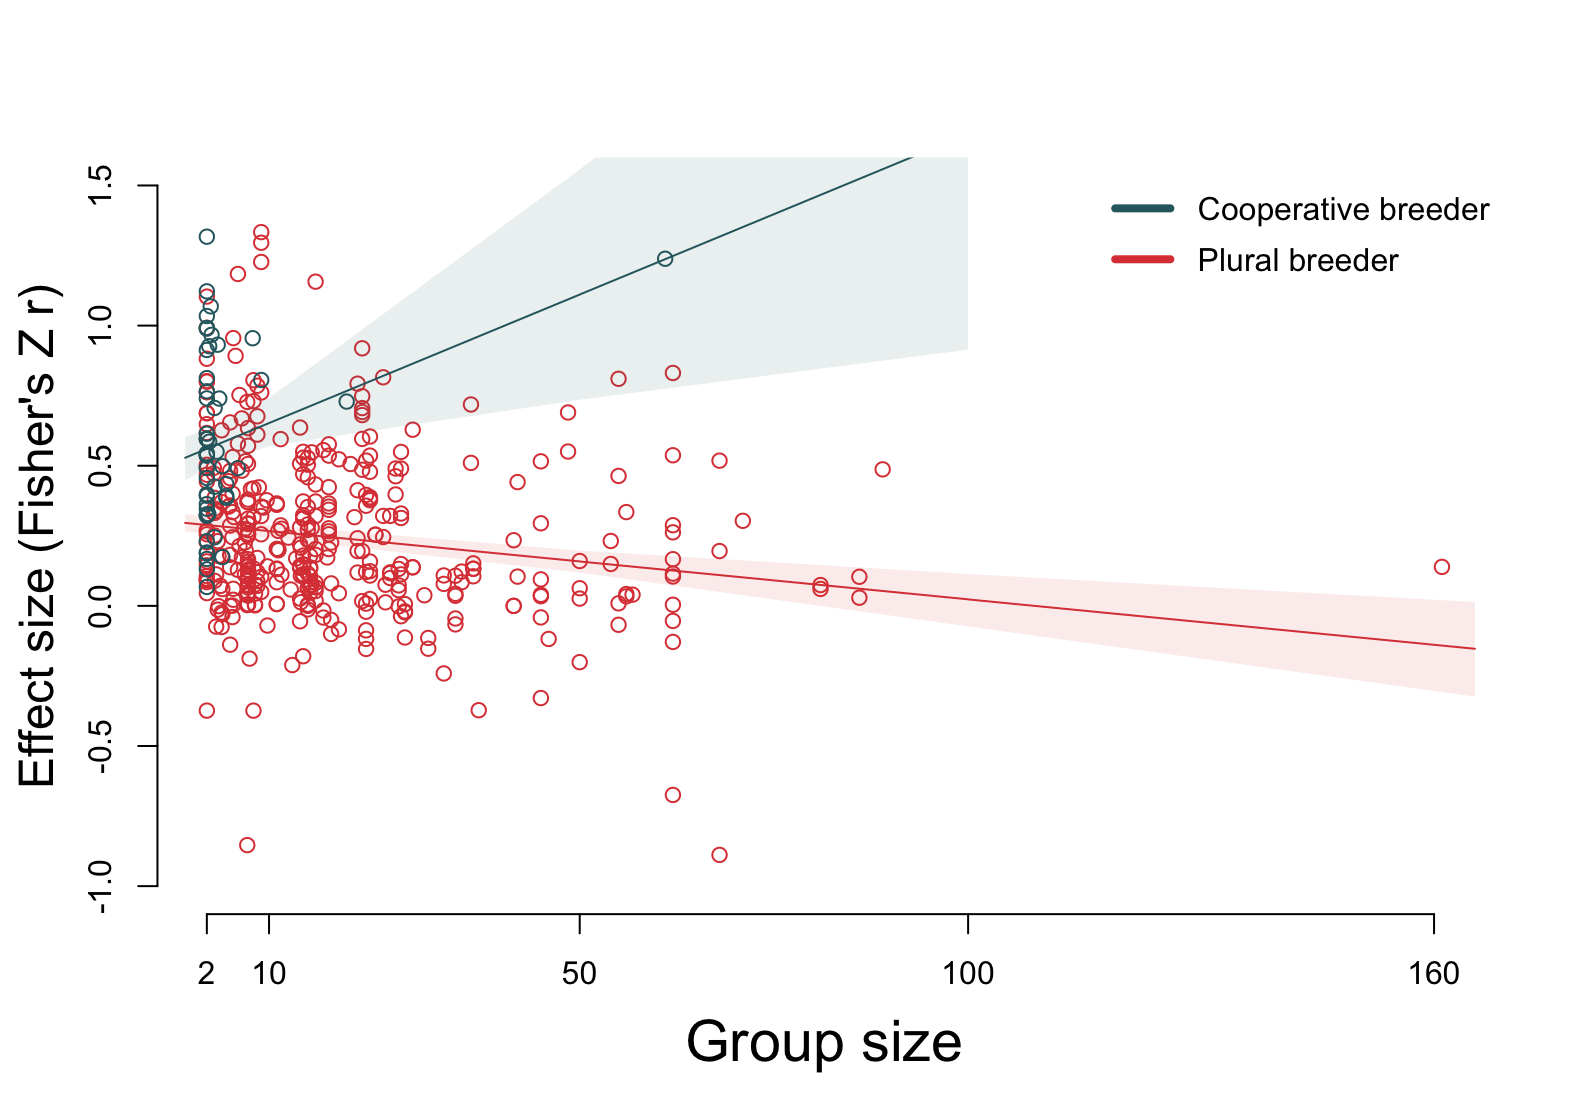
\includegraphics{ranksuccess_Fig8_effectsize_interaction_groupsize.png}
\textbf{Figure 9.} The relationship between the number of females in the
group and the effect of dominance on reproductive success depends on
whether the species is a cooperative (olive dots show data and olive
line with shading shows estimate from rethinking model) or a plural
breeder (red dots show data and red line with shading shows estimate
from rethinking model). In cooperative breeders, effect sizes increase
with increasing group size as a single female continues to monopolize
reproduction in the group, whereas effect sizes decrease with increasing
group size as dominants can potentially no longer control other females
in the group.

\begin{center}\rule{0.5\linewidth}{0.5pt}\end{center}

\textbf{R5.2.5 Average relatedness and cooperative breeding}

Similarly, there appears to be an interaction between average
relatedness and breeding systems (metafor estimate for cooperative
breeding -0.06 - +0.44, for average relatedness -0.75 - +0.03, for
interaction +0.10 - +1.51, n=288 effect sizes), with effect sizes
increasing with higher levels of average relatedness in cooperative
breeders (rethinking estimate 0.00 - +0.12, n=36 effect sizes) and
decreasing with higher levels of average relatedness in plural/associate
breeders (rethinking estimate -0.06 - 0.00, n=252 effect sizes)

\textbf{R5.2.6 Philopatry and cooperative breeding}

Female dispersal is more common in cooperative breeders (46\%) than in
plural/associated breeders (9\%). However, effect sizes are larger in
species with female dispersal also just among the plural/associated
breeders (rethinking estimate -0.19 - -0.02, n=363 effect sizes), though
differences between philopatry and dispersal are not associated with
effect sizes in cooperative breeders (rethinking estimate -0.10 - +0.12,
n=52 effect sizes) (metafor estimate for cooperative breeding +0.15 -
+0.49, for philopatry -0.18 - +0.06, for interaction -0.18 - +0.26).

\textbf{R5.2.7 Coalition formation and cooperative breeding}

Coalition formation does not occur in cooperative breeders, leading to a
potential confound. Restricting the analyses to plural/associated
breeders, we find that effect sizes are higher in species in which
females do form coalitions than in species where they do not (metafor
estimate 0.00 - +0.14, rethinking estimate +0.01 - +0.11, n=374 effect
sizes). This likely reflects the benefits of nepotism in matrilineal
groups. For our analysis, we did not differentiate between stabilizing
coalitions, which usually occur among kin to maintain matrilineal rank
differences, and revolutionary coalitions, which usually occur among
unrelated individuals to limit the power of others in the group.

~

\textbf{R5.3 Philopatry and group size}

Group sizes of species in which females disperse tend to be smaller than
group sizes of species in which females are philopatric. Both philopatry
and increasing group size appear however to independently lead to lower
effect sizes (metafor estimate philopatry -0.09 - -0.01 group size -0.07
- -0.01, rethinking estimate philopatry -0.16 - 0.00 group size -0.07 -
-0.03, n=415 effect sizes).

~

\textbf{R5.4 Philopatry and average relatedness}

Among plural/associated breeders, average relatedness is lower in
species in which females disperse (mean r 0.03, n=16) than in species in
which females are philopatric (mean r 0.10, n=228), and among these
species, differences in effect sizes are mainly associated with whether
females disperse or are philopatric (metafor estimate -0.11 - -0.03,
rethinking estimate -0.22 - -0.02) rather than levels of average
relatedness (metafor estimate +0.03 - +0.10, rethinking estimate -0.04 -
+0.01, n=242 effect sizes).

~

\textbf{R5.5 Population density and group size}

Population density and group size have independent influences on effect
sizes (population density estimate metafor 0.00 - +0.01, rethinking 0.00
- +0.01; group size estimate metafor -0.03 - 0.01, n=346 effect sizes).

~

\textbf{R5.6 Different influences in captive and wild populations}

Models in which both the intercept and the slopes can vary according to
whether studies were performed in the wild or in captivity also showed
that there are no systematic differences of the effects of dominance
rank on reproductive success between populations in these settings (for
the different life history measurements and for cooperative breeding).

~

~

\hypertarget{summary-of-combined-analyses}{%
\paragraph{\texorpdfstring{\textbf{Summary of combined
analyses}}{Summary of combined analyses}}\label{summary-of-combined-analyses}}

\hfill\break
The analyses of combinations of predictors of the effect size of
dominance on rank on reproductive success show that most predictors have
a direct influence. However, we find that the approach authors used to
measure the effect does not lead to different estimates of the effect
size, it is rather that different approaches have been used in different
study systems. We also find that average relatedness might not directly
mitigate effect sizes, but that it is a co-variate of the breeding
system and whether females are philopatric or disperse. In addition, we
find some interactions, with group size having divergent influences
depending on the breeding system; and coalitions among females reducing
effect sizes among plural breeders.

~

\hypertarget{discussion}{%
\subsection{Discussion}\label{discussion}}

Our study finds that, in social mammals, dominant females have higher
reproductive success than lower-ranking females. Positive effects of
dominance rank are present for all our measures of life history and
among plural breeders, where data for all measures of life history
exist, are highest for life-time reproductive success. This suggests
that even if dominants might face some trade-offs (e.g.~higher stress
levels Cavigelli et al. (2003)), obtaining a high ranking position in a
social group leads to fitness benefits, though how females obtain these
benefits (e.g.~shorter interbirth intervals versus larger offspring)
differ between populations. Our meta-analysis also highlights several
factors associated with variation in the strength of the effect of
dominance rank on reproductive success, where social factors in
particular appear to have a modulating influence while variation in life
history and ecological factors appears of less importance. Despite a
consistent positive relationship between higher dominance rank and
higher reproductive success, the data we were able to bring together for
this study show some biases that suggest that further studies might
detect lower effects. Our investigation of sample bias indicates a
combination of publication bias, study system bias, and study time bias.
Unlike often claimed for meta-analyses, the over-representation of
positive findings in our case appears not to be primarily due to a
file-drawer problem of unpublished negative findings but due to
researchers targeting their efforts on feasible systems. Studies into
the potential mechanisms of female competition and reproductive
suppression have focused on species where there are clear differences in
reproductive success between dominants and subordinates. In addition,
obtaining reliable reproductive success data in long-lived mammals takes
particular effort, again likely limiting the systems that have been
studied to investigate the effects of dominance rank. We did find that
studies conducted for longer time periods show less variance in their
estimates, potentially because they also have larger sample sizes.
Alternatively, or in addition, studies conducted across longer time
frames might be less likely to show extreme effect size estimates
because natural changes in dominance rank and events that affect all
females equally (e.g.~infanticide Cheney et al. (2004)) occur relatively
regularly across a multi-year study, while estimates derived over short
time frames may over-estimate effect sizes.

Overall, we estimated an average effect of 0.28 of rank on reproductive
success. What does this mean? First, it is important to highlight that
this effect size reflects how well rank predicts reproductive success,
but not directly indicates how different the reproductive success of
high-ranking females is from that of low-ranking females. While the
effect of dominance has to be zero in groups where all females have
exactly the same reproductive success, an effect of zero is also found
in a group where there are large differences in reproductive success
across females which do not align with the females' dominance rank. Just
by chance, we would expect differences in reproductive success among
females in a social group and we could also expect that these
differences are associated with traits that might be used to classify
social rank. To assess whether the effects we detect are higher than
such random variation, we performed simulations. For this, we simulated
artificial groups of females reflecting macaques, the genus most common
in our sample. We assumed that each female in each group might have
between 0 to 8 offspring, with an average 2 (following a Poisson
distribution, so most females have 1 or 2 offspring). We performed
10,000 simulations of six groups of twelve females each (the median
group size in our data). When we set no association between rank and
reproductive success, less than 0.1\% of simulations showed an effect
size as high or higher than the 0.28 we observe in the data (Figure 10).
Effect sizes for a perfect association between each female's rank and
her reproductive success ranged between 0.75-0.95 (mean 0.88).
Simulations in which the two highest ranking females always have the
highest reproductive success while rank among lower ranking females no
longer is associated with success produces effect sizes close to what we
observe (mean 0.32), whereas values tend to be slightly lower if only
the highest ranking female consistently has the highest success (mean
0.18). These simulations cannot resolve whether high ranking females
have higher reproductive success because they obtained this position or
whether there are some traits that lead to both higher rank and higher
reproductive success - or whether they are simply the lucky ones (Snyder
and Ellner (2018)). However, the value of the overall effect size we
observe compared to those under random expectations indicates that
social rank has a particular association with reproductive success
beyond the random variation we expect in social groups.

\begin{center}\rule{0.5\linewidth}{0.5pt}\end{center}

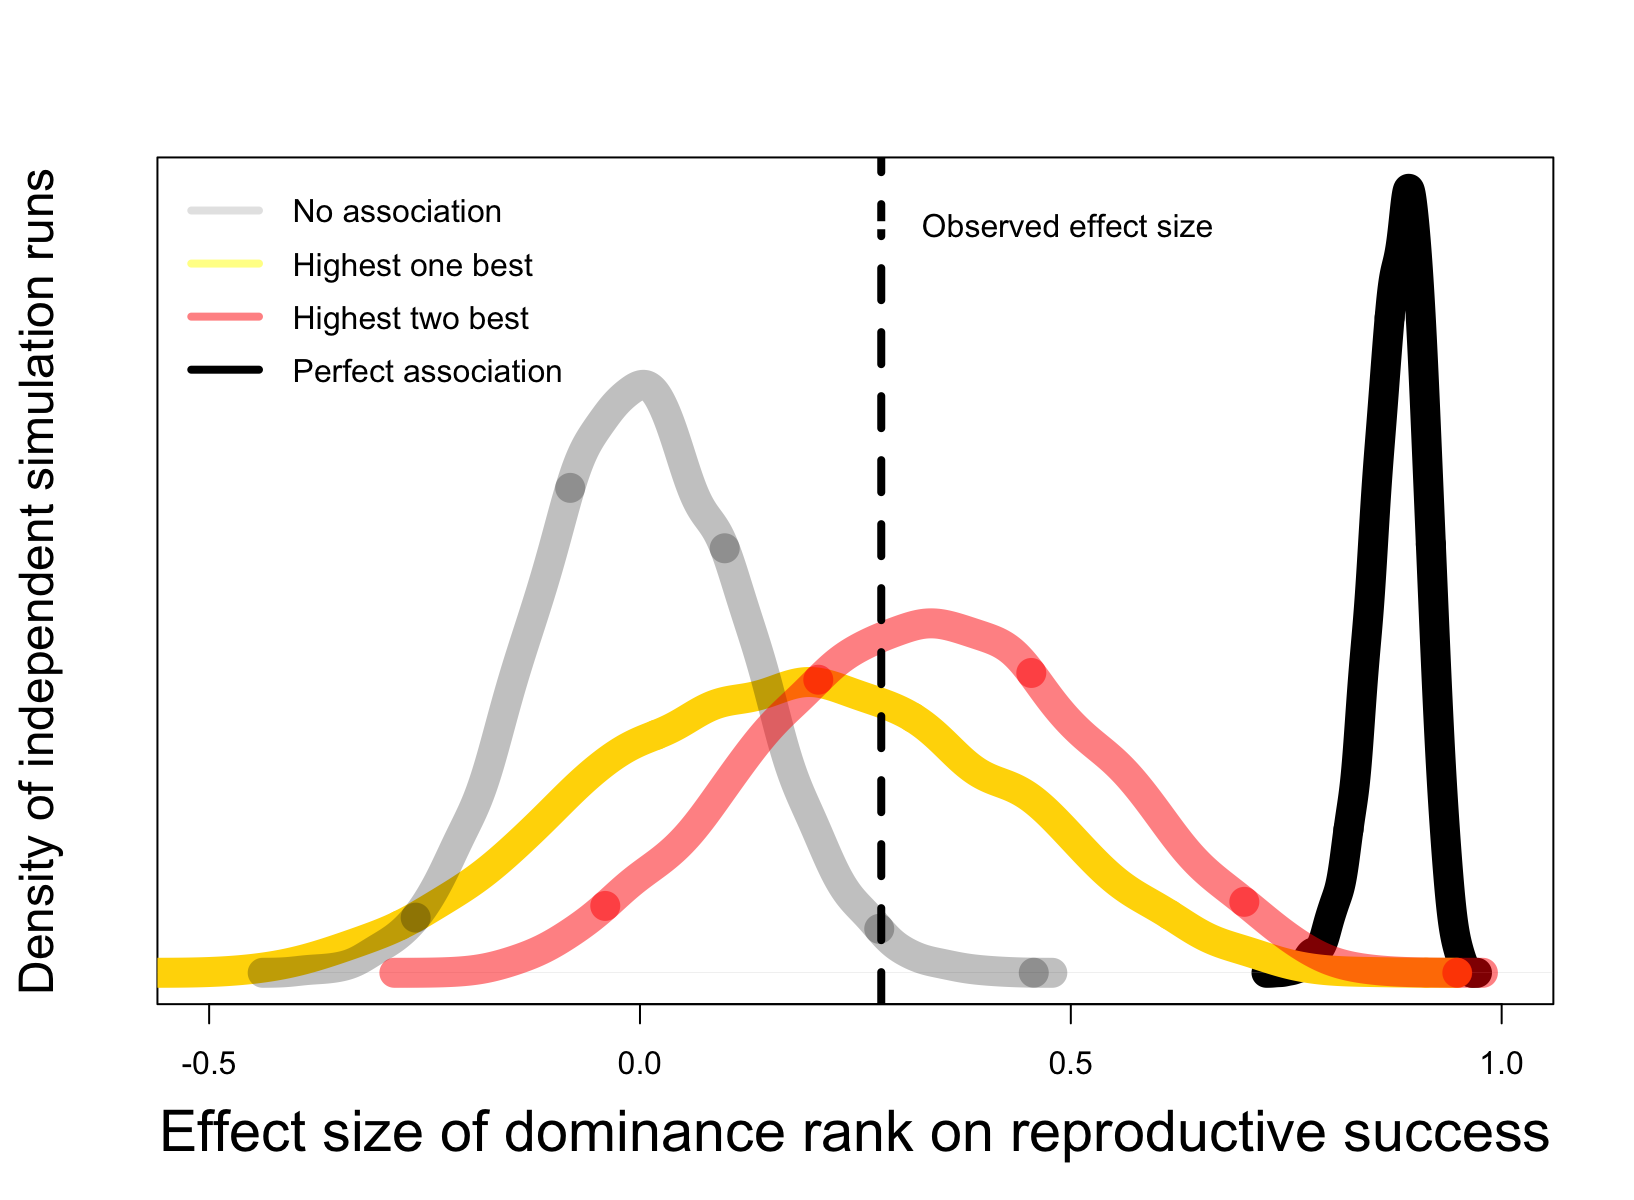
\includegraphics{ranksuccess_Fig10_simulatedeffectsizes.png}
\textbf{Figure 10.} The average effect size of dominance rank on female
reproductive success we observe in our sample (0.28; dotted vertical
line) is in between the effect sizes expected for social groups in which
there is either no (grey histogram) or a perfect association (black
histogram) between each rank and the reproductive success of females.
The observed value is close to a situation in which the two highest
ranking females (red histogram) or only the highest ranking female
(yellow histogram) always have the highest success in a group of twelve
females.

\begin{center}\rule{0.5\linewidth}{0.5pt}\end{center}

Among the social traits we investigated, the highest difference in the
effect of rank on reproductive success was between cooperative breeders
and plural/associated breeders. This results was expected given the
higher reproductive skew that has been found among females in
cooperative breeders (Lukas and Clutton-Brock (2012)). The contrast
between breeding systems appears due to the degree of reproductive
control that dominants in cooperative breeders have over their, mostly
related, group members. The likely importance of reproductive control of
dominant females in cooperative breeders compared to plural/associated
breeders are also reflected in the different relationships of the effect
sizes with group size in the different breeding systems. While among
cooperative breeders there usually is only a single breeding dominant
female and large groups occur when her reproductive output is higher,
dominant females in plural/associated breeders likely face reduced
opportunities to control reproduction in larger groups (Rubenstein,
Botero, and Lacey (2016)). In this context, it is again important to
note that we only look at the association between rank and the variation
in reproductive success within groups. Even though the relative
difference between dominant and subordinate females might be lower in
larger group sizes, in terms of overall fitness it might still be better
to be the dominant in a group of the optimal size rather than a smaller
group (e.g.~small group where dominant has 3 versus subordinate has 2
offspring (50\% higher fitness) compared to large group where dominant
has 4 while all other females have 3 offspring (33\% higher fitness)).
While reproductive control appears important in explaining high
reproductive success of dominant females, we did not find that
associations between the effect sizes and how females acquire and
maintain rank. Effect sizes were similar when dominant females acquire
their position by kin support versus aggression or age, and among
macaque species were not associated with dominance styles.

Among plural and associated breeders, effects of dominance rank on
female reproductive success are higher when (i) females disperse, (ii)
groups are smaller, and (iii) females form coalitions. These
observations are somewhat opposite to the processes presumably linked to
reproductive suppression in cooperative breeders. In addition, these
findings also do not support accounts that focus on nepotism as a
primary factor in leading to social groups with large differences among
females. It appears that in situations of strong nepotism females in a
group might have more similar reproductive success, with patterns such
as youngest sister ascendancy potentially reducing differences among kin
(Datta (1988), Bergstrom and Fedigan (2010), Lea et al. (2014)).
Instead, these findings suggest that competition among females might be
highest in social groups in which females form complex relationships and
rates of aggression are high (Lukas and Clutton-Brock (2018)). In our
sample we for example observe relative strong effects of high dominance
rank on reproductive success among equids and among gorillas, who have
similar social systems with females benefiting from forming social bonds
with unfamiliar/unrelated individuals they encounter when joining new
small groups upon reaching maturity (e.g. Cameron, Setsaas, and
Linklater (2009)).

Of the ecological variables we investigated, only population density was
associated with differences in effect sizes of dominance rank on
reproductive success, again supporting the role of social interactions
in shaping fitness outcomes of dominance interactions. The observation
that other ecological factors do not mitigate the strength of the
fitness benefit dominant females receive might suggests that dominants
are consistently able to outcompete other females in the group rather
than dominance only being important under challenging conditions. While
local ecological conditions, rather than the species-level traits we
used, might modulate fitness benefits of high dominance rank for
females, it seems unlikely that there would be a strong directional
influence given that effect sizes from the same species tend to be
similar, even in captive conditions. In line with this, previous work
has shown that subordinate females may not always be the first to suffer
under limiting conditions (Fedigan (1983)). Instead, a number of
ecological challenges, such as for example predation (Cheney et al.
(2004)), can affect all females independent of their rank and thereby
diminishing the relative benefits dominant females acquire (Altmann and
Alberts (2003)).

The overall effect size of dominance rank on female reproductive success
across the species in our sample is slightly higher than that reported
in a previous study, though we find a similar value when we restrict our
sample to primate species, the focus of the previous study (the average
in our sample is 0.28, for only the primates in our sample 0.23, versus
previously reported for primates 0.20 Majolo et al. (2012)). These
estimates of the effects of female dominance rank are lower than those
previously reported for males. The previous study on primates reports an
effect of male dominance rank on fecundity of 0.71 (Majolo et al.
(2012)), and estimates in a different study of the effect of dominance
rank on males' mating success are \textasciitilde0.6 (Cowlishaw and
Dunbar (1991)). Do these different estimates reflect that males benefit
more from high dominance rank than females? We think that we cannot make
such an inference at this stage. Measures of mating success might not
necessarily translate in equally high skew in reproductive success and
studies measuring male reproductive success tend to cover even shorter
time periods than the studies that identify female reproductive success.
Several of the factors we identified here to modulate the effect of
dominance rank on reproductive success may also be linked to differences
between females and males. However, it could be expected that males
benefit more from rank than females, given that females are more
monopolizable than many other resources. The benefits of rank are very
different in nature between males and females and only additional
symmetrical meta-analyses in males can answer such a question.

Our findings highlight that social factors can have important influences
on demography and genetic evolution by leading to systematic differences
in reproductive success. The effect of high dominance rank on
reproductive success influence the growth and composition of social
groups across generations. In particular when social rank is heritable,
strong long-term changes are visible in the few studies which have been
able to track reproductive success across multiple generations. For
example, among spotted hyenas, the highest ranking female in 1979 is the
ancestor of more than half of the females in the clan in 2009 (Holekamp
et al. (2012)). This perspective also highlights that even small
differences in reproductive success can add up over long time frames. In
particular, even if dominant females do not have much higher
reproduction under average conditions, if they were the only ones to
survive or reproduce under extreme conditions this could have important
fitness consequences (Lewontin and Cohen (1969)). For future studies,
detailed long-term investigations are not only relevant to understand
the long-term consequences of the effect of dominance rank on
reproduction, but also to infer the multiple mechanisms that link rank
to reproductive output (e.g. Fedigan (1983), Pusey, Williams, and
Goodall (1997)).

\hypertarget{ethics}{%
\subsubsection{Ethics}\label{ethics}}

Our study relies on previously published data.

\hypertarget{author-contributions}{%
\subsubsection{Author contributions}\label{author-contributions}}

\textbf{Shivani:} Hypothesis development, data collection, data analysis
and interpretation, revising/editing.

\textbf{Huchard:} Hypothesis development, data analysis and
interpretation, write up, revising/editing.

\textbf{Lukas:} Hypothesis development, data collection, data analysis
and interpretation, write up, revising/editing, materials/funding.

\hypertarget{funding}{%
\subsubsection{Funding}\label{funding}}

Shivani received funding from the INSPIRE programme of the Department of
Science \& Technology of the Government of India. This research was
supported by the Department of Human Behavior, Ecology and Culture at
the Max Planck Institute for Evolutionary Anthropology.

\hypertarget{conflict-of-interest-disclosure}{%
\subsubsection{Conflict of interest
disclosure}\label{conflict-of-interest-disclosure}}

We, the authors, declare that we have no financial conflicts of interest
with the content of this article. Elise Huchard and Dieter Lukas are
Recommenders at PCI Ecology.

~

\hypertarget{acknowledgements}{%
\subsubsection{Acknowledgements}\label{acknowledgements}}

We thank our PCI Ecology Recommender, Matthieu Paquet, and our
reviewers, Bonaventura Majolo and one anonymous reviewer, for their
valuable feedback that greatly improved this piece of research. We are
grateful to the members of the Department of Human Behavior, Ecology and
Culture at the Max Planck Institute for Evolutionary Anthropology for
feedback during the early stages of this project.

~

\hypertarget{references}{%
\subsubsection{\texorpdfstring{\href{MyLibrary.bib}{References}}{References}}\label{references}}

\begin{verbatim}
## Loading required namespace: bibtex
\end{verbatim}

\begin{verbatim}
## Writing 245 Bibtex entries ... OK
## Results written to file 'supplementalreferences.bib'
\end{verbatim}

\begin{tabu} to \linewidth {>{\raggedleft}X>{\raggedright}X>{\raggedright}X>{\raggedright}X>{\raggedright}X}
\hline
Effect size id & Species & Reference for Dominance Rank Effect & Reference for Dominance System & Reference for Average Relatedness\\
\hline
1 & Cervus\_elaphus & (Clutton-Brock, Albon, and Guinness, 1984) & (HALL, 2010) & (NUSSEY, COLTMAN, COULSON, KRUUK, DONALD, MORRIS, CLUTTON-BROCK, and PEMBERTON, 2005)\\
\hline
2 & Crocuta\_crocuta & (Holekamp, Smale, and Szykman, 1996) & (Hofer and East, 2003) & (Horn, Engh, Scribner, Funk, and Holekamp, 2004)\\
\hline
3 & Macaca\_arctoides & (Nieuwenhuijsen, Lammers, de
Neef, and Slob, 1985) & (HOLEKAMP and SMALE, 1991) & NA\\
\hline
4 & Macaca\_fuscata & (Gouzoules, Gouzoules, and Fedigan, 1982) & @koyama2003matrilineal & (Baxter and Fedigan, 1979)\\
\hline
5 & Macaca\_fuscata & (Takahata, Suzuki, Agetsuma, Okayasu, Sugiura, Takahashi, Yamagiwa, Izawa, Furuichi, Hill, Maruhashi, Saito, Saito, and Sprague, 1998) & @koyama2003matrilineal & (Nakagawa, Matsubara, Shimooka, and Nishikawa, 2015)\\
\hline
6 & Macaca\_fuscata & (Takahata, Suzuki, Agetsuma, et al., 1998) & @koyama2003matrilineal & (Nakagawa, Matsubara, Shimooka, et al., 2015)\\
\hline
7 & Macaca\_fuscata & (Takahata, Suzuki, Agetsuma, et al., 1998) & @koyama2003matrilineal & (Nakagawa, Matsubara, Shimooka, et al., 2015)\\
\hline
8 & Macaca\_mulatta & (Drickamer, 1974) & (Deutsch and Lee, 1991) & NA\\
\hline
9 & Mandrillus\_sphinx & (Setchell, Charpentier, and Wickings, 2005) & @setchell2002reproductive & NA\\
\hline
10 & Papio\_cynocephalus & (, 2021) & (Packer, Collins, Sindimwo, and Goodall, 1995) & NA\\
\hline
11 & Papio\_cynocephalus & (Wasser, Norton, Kleindorfer, and Rhine, 2004) & (Packer, Collins, Sindimwo, et al., 1995) & (Wasser and Starling, 1988)\\
\hline
12 & Rangifer\_tarandus & (Holand, Weladji, Gj�stein, Kumpula, Smith, Nieminen, and R�ed, 2004) & (Holand, Gjøstein, Losvar, Kumpula, Smith, Røed, Nieminen, and Weladji, 2004) & (Djaković, Holand, Hovland, Røed, Weladji, Fjeldstad, and Nieminen, 2011)\\
\hline
13 & Callithrix\_jacchus & (Sousa, da
Rocha Albuquerque, da
Silva Albuquerque, Araujo, Yamamoto, and de
Fatima Arruda, 2005) & (Digby, 1995) & @nievergelt2000genetic\\
\hline
14 & Chlorocebus\_aethiops & (Fairbanks and McGuire, 1984) & (HOLEKAMP and SMALE, 1991) & (Fairbanks, Jorgensen, Bailey, Breidenthal, Grzywa, and Laudenslager, 2011)\\
\hline
15 & Chlorocebus\_aethiops & (Fairbanks and McGuire, 1984) & (HOLEKAMP and SMALE, 1991) & (Fairbanks, Jorgensen, Bailey, et al., 2011)\\
\hline
16 & Crocuta\_crocuta & (Holekamp, Smale, and Szykman, 1996) & (Hofer and East, 2003) & (Horn, Engh, Scribner, et al., 2004)\\
\hline
17 & Crocuta\_crocuta & (Holekamp, Smale, and Szykman, 1996) & (Hofer and East, 2003) & (Horn, Engh, Scribner, et al., 2004)\\
\hline
18 & Lemur\_catta & (Takahata, Koyama, Ichino, Miyamoto, Nakamichi, and Soma, 2007) & (Taylor and Sussman, 1985) & (Parga, Sauther, Cuozzo, Jacky, Gould, Sussman, Lawler, and Pastorini, 2015)\\
\hline
19 & Macaca\_fuscata & (Gouzoules, Gouzoules, and Fedigan, 1982) & @koyama2003matrilineal & (Baxter and Fedigan, 1979)\\
\hline
20 & Macaca\_fuscata & (Gouzoules, Gouzoules, and Fedigan, 1982) & @koyama2003matrilineal & (Baxter and Fedigan, 1979)\\
\hline
21 & Macaca\_fuscata & (Wolfe, 1984) & @koyama2003matrilineal & @koyama2003matrilineal\\
\hline
22 & Macaca\_sylvanus & (Kümmerli and Martin, 2005) & (Paul and Kuester, 1987) & (Kümmerli and Martin, 2008)\\
\hline
23 & Macaca\_sylvanus & (Kümmerli and Martin, 2005) & (Paul and Kuester, 1987) & (Kümmerli and Martin, 2008)\\
\hline
24 & Mesocricetus\_auratus & (Huck, Lisk, and McKay, 1988) & (Huck, Lisk, and McKay, 1988) & (Huck, Lisk, and McKay, 1988)\\
\hline
25 & Mesocricetus\_auratus & (Huck, Lisk, and McKay, 1988) & (Huck, Lisk, and McKay, 1988) & (Huck, Lisk, and McKay, 1988)\\
\hline
26 & Mesocricetus\_auratus & (Huck, Lisk, and McKay, 1988) & (Huck, Lisk, and McKay, 1988) & (Huck, Lisk, and McKay, 1988)\\
\hline
27 & Oreamnos\_americanus & (é and Festa-Bianchet, 2001) & (é, 2000) & (Shafer, Northrup, White, Boyce, é, and Coltman, 2012)\\
\hline
28 & Oryctolagus\_cuniculus & (von
Holst, Hutzelmeyer, Kaetzke, et al., 2002) & (von
Holst, Hutzelmeyer, Kaetzke, Khaschei, Rödel, and Schrutka, 2002) & (SURRIDGE, IBRAHIM, BELL, WEBB, RICO, and HEWITT, 1999)\\
\hline
29 & Oryctolagus\_cuniculus & (von
Holst, Hutzelmeyer, Kaetzke, et al., 2002) & (von
Holst, Hutzelmeyer, Kaetzke, et al., 2002) & (SURRIDGE, IBRAHIM, BELL, et al., 1999)\\
\hline
30 & Papio\_cynocephalus & (Wasser, Norton, Kleindorfer, et al., 2004) & (Packer, Collins, Sindimwo, et al., 1995) & (Wasser and Starling, 1988)\\
\hline
31 & Semnopithecus\_entellus & (Borries, Sommer, and Srivastava, 1991) & (Borries, Sommer, and Srivastava, 1991) & NA\\
\hline
32 & Rangifer\_tarandus & (Holand, Weladji, Gj�stein, et al., 2004) & (Holand, Gjøstein, Losvar, et al., 2004) & (Djaković, Holand, Hovland, et al., 2011)\\
\hline
33 & Sciurus\_vulgaris & (Wauters and Dhondt, 1989) & (Wauters and Dhondt, 1989) & NA\\
\hline
34 & Sciurus\_vulgaris & (Wauters and Dhondt, 1989) & (Wauters and Dhondt, 1989) & NA\\
\hline
35 & Theropithecus\_gelada & (DUNBAR and DUNBAR, 1977) & (Dunbar, 1980) & (Snyder-Mackler, Alberts, and Bergman, 2014)\\
\hline
36 & Papio\_ursinus & @cheney2006reproduction & (HOLEKAMP and SMALE, 1991) & (Silk, Cheney, and Seyfarth, 1999)\\
\hline
37 & Papio\_ursinus & (Bulger and Hamilton, 1987) & (HOLEKAMP and SMALE, 1991) & (Silk, Cheney, and Seyfarth, 1999)\\
\hline
38 & Papio\_ursinus & (Bulger and Hamilton, 1987) & (HOLEKAMP and SMALE, 1991) & (Silk, Cheney, and Seyfarth, 1999)\\
\hline
39 & Cervus\_elaphus & (Clutton-Brock, Albon, and Guinness, 1984) & (HALL, 2010) & (NUSSEY, COLTMAN, COULSON, et al., 2005)\\
\hline
40 & Crocuta\_crocuta & (Holekamp, Smale, and Szykman, 1996) & (Hofer and East, 2003) & (Horn, Engh, Scribner, et al., 2004)\\
\hline
41 & Gorilla\_beringei & (Robbins, Robbins, Gerald-Steklis, and Steklis, 2007) & (Robbins, Gerald-Steklis, Robbins, and Steklis, 2005) & (Watts, 1994)\\
\hline
42 & Lemur\_catta & (Takahata, Koyama, Ichino, et al., 2007) & (Taylor and Sussman, 1985) & (Parga, Sauther, Cuozzo, et al., 2015)\\
\hline
43 & Macaca\_fascicularis & (van
Noordwijk and van
Schaik, 1999) & (van
Noordwijk and van
Schaik, 1987) & (Ruiter and Geffen, 1998)\\
\hline
44 & Macaca\_fascicularis & (van
Noordwijk and van
Schaik, 1999) & (van
Noordwijk and van
Schaik, 1987) & (Ruiter and Geffen, 1998)\\
\hline
45 & Macaca\_fascicularis & (van
Noordwijk and van
Schaik, 1999) & (van
Noordwijk and van
Schaik, 1987) & (Ruiter and Geffen, 1998)\\
\hline
46 & Macaca\_fascicularis & (van
Noordwijk and van
Schaik, 1999) & (van
Noordwijk and van
Schaik, 1987) & (Ruiter and Geffen, 1998)\\
\hline
47 & Macaca\_fascicularis & (van
Noordwijk and van
Schaik, 1999) & (van
Noordwijk and van
Schaik, 1987) & (Ruiter and Geffen, 1998)\\
\hline
48 & Macaca\_fascicularis & (van
Noordwijk and van
Schaik, 1999) & (van
Noordwijk and van
Schaik, 1987) & (Ruiter and Geffen, 1998)\\
\hline
49 & Macaca\_fascicularis & (van
Noordwijk and van
Schaik, 1999) & (van
Noordwijk and van
Schaik, 1987) & (Ruiter and Geffen, 1998)\\
\hline
50 & Macaca\_fascicularis & (van
Noordwijk and van
Schaik, 1999) & (van
Noordwijk and van
Schaik, 1987) & (Ruiter and Geffen, 1998)\\
\hline
51 & Macaca\_fascicularis & (van
Noordwijk and van
Schaik, 1999) & (van
Noordwijk and van
Schaik, 1987) & (Ruiter and Geffen, 1998)\\
\hline
52 & Macaca\_fascicularis & (van
Noordwijk and van
Schaik, 1999) & (van
Noordwijk and van
Schaik, 1987) & (Ruiter and Geffen, 1998)\\
\hline
53 & Macaca\_fascicularis & (van
Noordwijk and van
Schaik, 1999) & (van
Noordwijk and van
Schaik, 1987) & (Ruiter and Geffen, 1998)\\
\hline
54 & Macaca\_fascicularis & (van
Noordwijk and van
Schaik, 1999) & (van
Noordwijk and van
Schaik, 1987) & (Ruiter and Geffen, 1998)\\
\hline
55 & Macaca\_fascicularis & (van
Noordwijk and van
Schaik, 1999) & (van
Noordwijk and van
Schaik, 1987) & (Ruiter and Geffen, 1998)\\
\hline
56 & Macaca\_fascicularis & (van
Noordwijk and van
Schaik, 1999) & (van
Noordwijk and van
Schaik, 1987) & (Ruiter and Geffen, 1998)\\
\hline
57 & Macaca\_fascicularis & (van
Noordwijk and van
Schaik, 1999) & (van
Noordwijk and van
Schaik, 1987) & (Ruiter and Geffen, 1998)\\
\hline
58 & Macaca\_fascicularis & (van
Noordwijk and van
Schaik, 1999) & (van
Noordwijk and van
Schaik, 1987) & (Ruiter and Geffen, 1998)\\
\hline
59 & Macaca\_fascicularis & (van
Noordwijk and van
Schaik, 1999) & (van
Noordwijk and van
Schaik, 1987) & (Ruiter and Geffen, 1998)\\
\hline
60 & Macaca\_fascicularis & (van
Noordwijk and van
Schaik, 1999) & (van
Noordwijk and van
Schaik, 1987) & (Ruiter and Geffen, 1998)\\
\hline
61 & Macaca\_fascicularis & (van
Noordwijk and van
Schaik, 1999) & (van
Noordwijk and van
Schaik, 1987) & (Ruiter and Geffen, 1998)\\
\hline
62 & Macaca\_fascicularis & (van
Noordwijk and van
Schaik, 1999) & (van
Noordwijk and van
Schaik, 1987) & (Ruiter and Geffen, 1998)\\
\hline
63 & Macaca\_fascicularis & (van
Noordwijk and van
Schaik, 1999) & (van
Noordwijk and van
Schaik, 1987) & (Ruiter and Geffen, 1998)\\
\hline
64 & Macaca\_fuscata & (Takahata, Suzuki, Agetsuma, et al., 1998) & @koyama2003matrilineal & (Nakagawa, Matsubara, Shimooka, et al., 2015)\\
\hline
65 & Macaca\_mulatta & (Meikle and Vessey, 1988) & (Deutsch and Lee, 1991) & NA\\
\hline
66 & Oreamnos\_americanus & (é and Festa-Bianchet, 2001) & (é, 2000) & (Shafer, Northrup, White, et al., 2012)\\
\hline
67 & Oreamnos\_americanus & (é and Festa-Bianchet, 2001) & (é, 2000) & (Shafer, Northrup, White, et al., 2012)\\
\hline
68 & Oryctolagus\_cuniculus & (von
Holst, Hutzelmeyer, Kaetzke, et al., 2002) & (von
Holst, Hutzelmeyer, Kaetzke, et al., 2002) & (SURRIDGE, IBRAHIM, BELL, et al., 1999)\\
\hline
69 & Pan\_troglodytes & (Pusey, 1997) & @wittig2003food & (Vigilant, Hofreiter, Siedel, and Boesch, 2001)\\
\hline
70 & Papio\_anubis & (Packer, Collins, Sindimwo, et al., 1995) & (Johnson, 1987) & @kopp2015gene\\
\hline
71 & Papio\_anubis & (Packer, Collins, Sindimwo, et al., 1995) & (Johnson, 1987) & @kopp2015gene\\
\hline
72 & Papio\_anubis & (Packer, Collins, Sindimwo, et al., 1995) & (Johnson, 1987) & @kopp2015gene\\
\hline
73 & Papio\_anubis & (Packer, Collins, Sindimwo, et al., 1995) & (Johnson, 1987) & @kopp2015gene\\
\hline
74 & Papio\_anubis & (Packer, Collins, Sindimwo, et al., 1995) & (Johnson, 1987) & @kopp2015gene\\
\hline
75 & Papio\_cynocephalus & (Wasser, Norton, Kleindorfer, et al., 2004) & (Packer, Collins, Sindimwo, et al., 1995) & (Wasser and Starling, 1988)\\
\hline
76 & Papio\_cynocephalus & (Silk, 2003) & (Packer, Collins, Sindimwo, et al., 1995) & (Horn, Buchan, Altmann, and Alberts, 2007)\\
\hline
77 & Papio\_cynocephalus & (Silk, 2003) & (Packer, Collins, Sindimwo, et al., 1995) & (Horn, Buchan, Altmann, et al., 2007)\\
\hline
78 & Semnopithecus\_entellus & (Borries, Sommer, and Srivastava, 1991) & (Borries, Sommer, and Srivastava, 1991) & NA\\
\hline
79 & Semnopithecus\_entellus & (Borries, Sommer, and Srivastava, 1991) & (Borries, Sommer, and Srivastava, 1991) & NA\\
\hline
80 & Crocuta\_crocuta & (Hofer and East, 2003) & (Hofer and East, 2003) & NA\\
\hline
81 & Papio\_ursinus & @cheney2006reproduction & (HOLEKAMP and SMALE, 1991) & (Silk, Cheney, and Seyfarth, 1999)\\
\hline
82 & Papio\_ursinus & @cheney2006reproduction & (HOLEKAMP and SMALE, 1991) & (Silk, Cheney, and Seyfarth, 1999)\\
\hline
83 & Papio\_ursinus & (Bulger and Hamilton, 1987) & (HOLEKAMP and SMALE, 1991) & (Silk, Cheney, and Seyfarth, 1999)\\
\hline
84 & Papio\_ursinus & (Bulger and Hamilton, 1987) & (HOLEKAMP and SMALE, 1991) & (Silk, Cheney, and Seyfarth, 1999)\\
\hline
85 & Macaca\_fuscata & (Gouzoules, Gouzoules, and Fedigan, 1982) & @koyama2003matrilineal & (Baxter and Fedigan, 1979)\\
\hline
86 & Macaca\_fuscata & (Takahata, Suzuki, Agetsuma, et al., 1998) & @koyama2003matrilineal & (Nakagawa, Matsubara, Shimooka, et al., 2015)\\
\hline
87 & Mandrillus\_sphinx & @setchell2002reproductive & @setchell2002reproductive & NA\\
\hline
88 & Papio\_anubis & @cheney2006reproduction & (Johnson, 1987) & @kopp2015gene\\
\hline
89 & Papio\_ursinus & NA & (HOLEKAMP and SMALE, 1991) & (Silk, Cheney, and Seyfarth, 1999)\\
\hline
90 & Papio\_ursinus & @cheney2006reproduction & (HOLEKAMP and SMALE, 1991) & (Silk, Cheney, and Seyfarth, 1999)\\
\hline
91 & Chlorocebus\_aethiops & (Fairbanks and McGuire, 1984) & (HOLEKAMP and SMALE, 1991) & (Fairbanks, Jorgensen, Bailey, et al., 2011)\\
\hline
92 & Crocuta\_crocuta & (Holekamp, Smale, and Szykman, 1996) & (Hofer and East, 2003) & (Horn, Engh, Scribner, et al., 2004)\\
\hline
93 & Crocuta\_crocuta & (Holekamp, Smale, and Szykman, 1996) & (Hofer and East, 2003) & (Horn, Engh, Scribner, et al., 2004)\\
\hline
94 & Crocuta\_crocuta & (Holekamp, Smale, and Szykman, 1996) & (Hofer and East, 2003) & (Horn, Engh, Scribner, et al., 2004)\\
\hline
95 & Crocuta\_crocuta & (Holekamp, Smale, and Szykman, 1996) & (Hofer and East, 2003) & (Horn, Engh, Scribner, et al., 2004)\\
\hline
96 & Crocuta\_crocuta & (Holekamp, Smale, and Szykman, 1996) & (Hofer and East, 2003) & (Horn, Engh, Scribner, et al., 2004)\\
\hline
97 & Gorilla\_beringei & (Robbins, Robbins, Gerald-Steklis, et al., 2007) & (Robbins, Gerald-Steklis, Robbins, et al., 2005) & (Watts, 1994)\\
\hline
98 & Macaca\_arctoides & (Nieuwenhuijsen, Lammers, de
Neef, et al., 1985) & (HOLEKAMP and SMALE, 1991) & NA\\
\hline
99 & Mandrillus\_sphinx & @setchell2002reproductive & @setchell2002reproductive & NA\\
\hline
100 & Mandrillus\_sphinx & @setchell2002reproductive & @setchell2002reproductive & NA\\
\hline
101 & Papio\_anubis & (Packer, Collins, Sindimwo, et al., 1995) & (Johnson, 1987) & NA\\
\hline
102 & Papio\_anubis & (Packer, Collins, Sindimwo, et al., 1995) & (Johnson, 1987) & @kopp2015gene\\
\hline
103 & Papio\_anubis & (Packer, Collins, Sindimwo, et al., 1995) & (Johnson, 1987) & @kopp2015gene\\
\hline
104 & Papio\_anubis & (Packer, Collins, Sindimwo, et al., 1995) & (Johnson, 1987) & @kopp2015gene\\
\hline
105 & Papio\_anubis & (Garcia, Lee, and Rosetta, 2006) & (Johnson, 1987) & NA\\
\hline
106 & Papio\_anubis & (Garcia, Lee, and Rosetta, 2006) & (Johnson, 1987) & NA\\
\hline
107 & Papio\_cynocephalus & (Wasser, Norton, Kleindorfer, et al., 2004) & (Packer, Collins, Sindimwo, et al., 1995) & (Wasser and Starling, 1988)\\
\hline
108 & Papio\_cynocephalus & (Wasser, Norton, Kleindorfer, et al., 2004) & (Packer, Collins, Sindimwo, et al., 1995) & (Wasser and Starling, 1988)\\
\hline
109 & Papio\_cynocephalus & (Wasser, Norton, Kleindorfer, et al., 2004) & (Packer, Collins, Sindimwo, et al., 1995) & (Wasser and Starling, 1988)\\
\hline
110 & Papio\_anubis & (Barton and Whiten, 1993) & (Johnson, 1987) & @lynch2016paternal\\
\hline
111 & Papio\_ursinus & (Bulger and Hamilton, 1987) & (HOLEKAMP and SMALE, 1991) & (Silk, Cheney, and Seyfarth, 1999)\\
\hline
112 & Papio\_ursinus & (Bulger and Hamilton, 1987) & (HOLEKAMP and SMALE, 1991) & (Silk, Cheney, and Seyfarth, 1999)\\
\hline
113 & Gorilla\_beringei & (Robbins, Robbins, Gerald-Steklis, et al., 2007) & (Robbins, Gerald-Steklis, Robbins, et al., 2005) & (Watts, 1994)\\
\hline
114 & Macaca\_fascicularis & (van
Noordwijk and van
Schaik, 1999) & (van
Noordwijk and van
Schaik, 1987) & (Ruiter and Geffen, 1998)\\
\hline
115 & Macaca\_fascicularis & (van
Noordwijk and van
Schaik, 1999) & (van
Noordwijk and van
Schaik, 1987) & (Ruiter and Geffen, 1998)\\
\hline
116 & Macaca\_fascicularis & (van
Noordwijk and van
Schaik, 1999) & (van
Noordwijk and van
Schaik, 1987) & (Ruiter and Geffen, 1998)\\
\hline
117 & Macaca\_fascicularis & (van
Noordwijk and van
Schaik, 1999) & (van
Noordwijk and van
Schaik, 1987) & (Ruiter and Geffen, 1998)\\
\hline
118 & Macaca\_fascicularis & (van
Noordwijk and van
Schaik, 1999) & (van
Noordwijk and van
Schaik, 1987) & (Ruiter and Geffen, 1998)\\
\hline
119 & Macaca\_fascicularis & (van
Noordwijk and van
Schaik, 1999) & (van
Noordwijk and van
Schaik, 1987) & (Ruiter and Geffen, 1998)\\
\hline
120 & Macaca\_fascicularis & (van
Noordwijk and van
Schaik, 1999) & (van
Noordwijk and van
Schaik, 1987) & (Ruiter and Geffen, 1998)\\
\hline
121 & Macaca\_fascicularis & (van
Noordwijk and van
Schaik, 1999) & (van
Noordwijk and van
Schaik, 1987) & (Ruiter and Geffen, 1998)\\
\hline
122 & Macaca\_fuscata & (Takahata, Suzuki, Agetsuma, et al., 1998) & @koyama2003matrilineal & (Nakagawa, Matsubara, Shimooka, et al., 2015)\\
\hline
123 & Macaca\_fuscata & (Takahata, Suzuki, Agetsuma, et al., 1998) & @koyama2003matrilineal & (Nakagawa, Matsubara, Shimooka, et al., 2015)\\
\hline
124 & Macaca\_fuscata & (Takahata, Suzuki, Agetsuma, et al., 1998) & @koyama2003matrilineal & (Nakagawa, Matsubara, Shimooka, et al., 2015)\\
\hline
125 & Macaca\_fuscata & (Takahata, Suzuki, Agetsuma, et al., 1998) & @koyama2003matrilineal & (Nakagawa, Matsubara, Shimooka, et al., 2015)\\
\hline
126 & Mandrillus\_sphinx & (Setchell, Charpentier, and Wickings, 2005) & @setchell2002reproductive & NA\\
\hline
127 & Ovis\_canadensis & (Festa-Bianchet, 1991) & (Festa-Bianchet, 1991) & (Fournier and Festa-Bianchet, 1995)\\
\hline
128 & Papio\_anubis & (Packer, Collins, Sindimwo, et al., 1995) & (Johnson, 1987) & @kopp2015gene\\
\hline
129 & Papio\_anubis & (Packer, Collins, Sindimwo, et al., 1995) & (Johnson, 1987) & @kopp2015gene\\
\hline
130 & Papio\_cynocephalus & (Wasser, Norton, Kleindorfer, et al., 2004) & (Packer, Collins, Sindimwo, et al., 1995) & (Wasser and Starling, 1988)\\
\hline
131 & Crocuta\_crocuta & (Hofer and East, 2003) & (Hofer and East, 2003) & NA\\
\hline
132 & Macaca\_fuscata & (Takahata, 1980) & @koyama2003matrilineal & @koyama2003matrilineal\\
\hline
133 & Oryctolagus\_cuniculus & (von
Holst, Hutzelmeyer, Kaetzke, et al., 2002) & (von
Holst, Hutzelmeyer, Kaetzke, et al., 2002) & (SURRIDGE, IBRAHIM, BELL, et al., 1999)\\
\hline
134 & Papio\_anubis & (Packer, Collins, Sindimwo, et al., 1995) & (Johnson, 1987) & @kopp2015gene\\
\hline
135 & Papio\_anubis & (Packer, Collins, Sindimwo, et al., 1995) & (Johnson, 1987) & @kopp2015gene\\
\hline
136 & Papio\_cynocephalus & (Wasser, Norton, Kleindorfer, et al., 2004) & (Packer, Collins, Sindimwo, et al., 1995) & (Wasser and Starling, 1988)\\
\hline
137 & Papio\_cynocephalus & (Wasser, Norton, Kleindorfer, et al., 2004) & (Packer, Collins, Sindimwo, et al., 1995) & (Wasser and Starling, 1988)\\
\hline
138 & Papio\_cynocephalus & (Wasser, Norton, Kleindorfer, et al., 2004) & (Packer, Collins, Sindimwo, et al., 1995) & (Wasser and Starling, 1988)\\
\hline
139 & Crocuta\_crocuta & (Hofer and East, 2003) & (Hofer and East, 2003) & NA\\
\hline
140 & Papio\_ursinus & @cheney2006reproduction & (HOLEKAMP and SMALE, 1991) & (Silk, Cheney, and Seyfarth, 1999)\\
\hline
141 & Papio\_ursinus & @cheney2006reproduction & (HOLEKAMP and SMALE, 1991) & (Silk, Cheney, and Seyfarth, 1999)\\
\hline
142 & Cervus\_elaphus & (Clutton-Brock, Albon, and Guinness, 1984) & (HALL, 2010) & (NUSSEY, COLTMAN, COULSON, et al., 2005)\\
\hline
143 & Cervus\_elaphus & (Clutton-Brock, Albon, and Guinness, 1984) & (HALL, 2010) & (NUSSEY, COLTMAN, COULSON, et al., 2005)\\
\hline
144 & Macaca\_mulatta & (Wilson, Gordon, and Bernstein, 1978) & (Deutsch and Lee, 1991) & (Bernstein and Ehardt, 1986)\\
\hline
145 & Macaca\_mulatta & (Wilson, Gordon, and Bernstein, 1978) & (Deutsch and Lee, 1991) & (Bernstein and Ehardt, 1986)\\
\hline
146 & Macaca\_sinica & (Dittus, 1979) & (Dittus, 1986) & NA\\
\hline
147 & Macaca\_sinica & (Dittus, 1979) & (Dittus, 1986) & NA\\
\hline
148 & Lycaon\_pictus & (Creel, Creel, Mills, and Monfort, 1997) & (Spiering, Somers, Maldonado, Wildt, and Gunther, 2009) & (Girman, Mills, Geffen, and Wayne, 1997)\\
\hline
149 & Fukomys\_damarensis & (BURLAND, BENNETT, JARVIS, and FAULKES, 2004) & (Gaylard, Harrison, and Bennett, 1998) & (Burland, Bennett, Jarvis, and Faulkes, 2002)\\
\hline
150 & Macaca\_fuscata & (Fedigan, Fedigan, Gouzoules, Gouzoules, and Koyama, 1986) & @koyama2003matrilineal & (Baxter and Fedigan, 1979)\\
\hline
151 & Macaca\_fuscata & (Fedigan, Fedigan, Gouzoules, et al., 1986) & @koyama2003matrilineal & (Baxter and Fedigan, 1979)\\
\hline
152 & Macaca\_fuscata & (Fedigan, Fedigan, Gouzoules, et al., 1986) & @koyama2003matrilineal & (Baxter and Fedigan, 1979)\\
\hline
153 & Macaca\_fuscata & (Fedigan, Fedigan, Gouzoules, et al., 1986) & @koyama2003matrilineal & (Baxter and Fedigan, 1979)\\
\hline
154 & Helogale\_parvula & (Keane, Waser, Creel, Creel, Elliott, and Minchella, 1994) & (Creel, 2005) & (Creel and Waser, 1994)\\
\hline
155 & Helogale\_parvula & (Keane, Waser, Creel, et al., 1994) & (Creel, 2005) & (Creel and Waser, 1994)\\
\hline
156 & Helogale\_parvula & (Keane, Waser, Creel, et al., 1994) & (Creel, 2005) & (Creel and Waser, 1994)\\
\hline
157 & Marmota\_caligata & (Wasser and Barash, 1983) & (Patil, Karels, and Hik, 2015) & NA\\
\hline
158 & Marmota\_caligata & (Wasser and Barash, 1983) & (Patil, Karels, and Hik, 2015) & NA\\
\hline
159 & Marmota\_caligata & (Wasser and Barash, 1983) & (Patil, Karels, and Hik, 2015) & NA\\
\hline
160 & Marmota\_caligata & (Wasser and Barash, 1983) & (Patil, Karels, and Hik, 2015) & NA\\
\hline
161 & Macaca\_radiata & (Silk, Clark-Wheatley, Rodman, and Samuels, 1981) & (HOLEKAMP and SMALE, 1991) & NA\\
\hline
162 & Macaca\_radiata & (Silk, Clark-Wheatley, Rodman, et al., 1981) & (HOLEKAMP and SMALE, 1991) & NA\\
\hline
163 & Macaca\_radiata & (Silk, Clark-Wheatley, Rodman, et al., 1981) & (HOLEKAMP and SMALE, 1991) & NA\\
\hline
164 & Marmota\_flaviventris & (Huang, Wey, and Blumstein, 2011) & (Huang, Wey, and Blumstein, 2011) & (Armitage, Vuren, Ozgul, and Oli, 2011)\\
\hline
165 & Marmota\_flaviventris & (Huang, Wey, and Blumstein, 2011) & (Huang, Wey, and Blumstein, 2011) & (Armitage, Vuren, Ozgul, et al., 2011)\\
\hline
166 & Marmota\_flaviventris & (Huang, Wey, and Blumstein, 2011) & (Huang, Wey, and Blumstein, 2011) & (Armitage, Vuren, Ozgul, et al., 2011)\\
\hline
167 & Marmota\_flaviventris & (Huang, Wey, and Blumstein, 2011) & (Huang, Wey, and Blumstein, 2011) & (Armitage, Vuren, Ozgul, et al., 2011)\\
\hline
168 & Alouatta\_palliata & (Glander, 1980) & (Jones, 1980) & NA\\
\hline
169 & Alouatta\_palliata & (Glander, 1980) & (Jones, 1980) & NA\\
\hline
170 & Equus\_quagga & (Pluháček, š, and Čul\textbackslash{}'\textbackslash{}ik, 2006) & (Lloyd and Rasa, 1994) & NA\\
\hline
171 & Equus\_quagga & (Pluháček, š, and Čul\textbackslash{}'\textbackslash{}ik, 2006) & (Lloyd and Rasa, 1994) & NA\\
\hline
172 & Equus\_zebra & (Lloyd and Rasa, 1989) & (Lloyd and Rasa, 1994) & NA\\
\hline
173 & Equus\_zebra & (Lloyd and Rasa, 1989) & (Lloyd and Rasa, 1994) & NA\\
\hline
174 & Equus\_zebra & (Lloyd and Rasa, 1989) & (Lloyd and Rasa, 1994) & NA\\
\hline
175 & Equus\_zebra & (Lloyd and Rasa, 1989) & (Lloyd and Rasa, 1994) & NA\\
\hline
176 & Equus\_zebra & (Lloyd and Rasa, 1989) & (Lloyd and Rasa, 1994) & NA\\
\hline
177 & Equus\_caballus & @rubenstein2009sociality & @sinderbrand2011relationship & NA\\
\hline
178 & Equus\_caballus & @rubenstein2009sociality & @sinderbrand2011relationship & NA\\
\hline
179 & Equus\_caballus & @rubenstein2009sociality & NA & NA\\
\hline
180 & Mirounga\_angustirostris & @cheney1988vervet & (Christenson and Boeuf, 1978) & NA\\
\hline
181 & Ovis\_canadensis & (Hass, 1991) & (Festa-Bianchet, 1991) & (Fournier and Festa-Bianchet, 1995)\\
\hline
182 & Ovis\_canadensis & (Hass, 1991) & (Festa-Bianchet, 1991) & (Fournier and Festa-Bianchet, 1995)\\
\hline
183 & Ovis\_canadensis & (Hass, 1991) & (Festa-Bianchet, 1991) & (Fournier and Festa-Bianchet, 1995)\\
\hline
184 & Hyaena\_brunnea & (OWENS and OWENS, 1996) & (OWENS and OWENS, 1996) & (Knowles, de
Groot, Wiesel, and Boag, 2009)\\
\hline
185 & Hyaena\_brunnea & (OWENS and OWENS, 1996) & (OWENS and OWENS, 1996) & (Knowles, de
Groot, Wiesel, et al., 2009)\\
\hline
186 & Mus\_musculus & (Rusu and Krackow, 2004) & (Rusu and Krackow, 2004) & (Rusu and Krackow, 2004)\\
\hline
187 & Mus\_musculus & (König, 1994) & (Rusu and Krackow, 2004) & (König, 1994)\\
\hline
188 & Mus\_musculus & (König, 1994) & (Rusu and Krackow, 2004) & (König, 1994)\\
\hline
189 & Mus\_musculus & (König, 1994) & (Rusu and Krackow, 2004) & (König, 1994)\\
\hline
190 & Mus\_musculus & (König, 1994) & (Rusu and Krackow, 2004) & (König, 1994)\\
\hline
191 & Rhabdomys\_pumilio & (Kinahan and Pillay, 2007) & (Kinahan and Pillay, 2007) & (Kinahan and Pillay, 2007)\\
\hline
192 & Rhabdomys\_pumilio & (Kinahan and Pillay, 2007) & (Kinahan and Pillay, 2007) & (Kinahan and Pillay, 2007)\\
\hline
193 & Rhabdomys\_pumilio & (Kinahan and Pillay, 2007) & (Kinahan and Pillay, 2007) & (Kinahan and Pillay, 2007)\\
\hline
194 & Rhabdomys\_pumilio & (Kinahan and Pillay, 2007) & (Kinahan and Pillay, 2007) & (Kinahan and Pillay, 2007)\\
\hline
195 & Rhabdomys\_pumilio & (Kinahan and Pillay, 2007) & (Kinahan and Pillay, 2007) & (Kinahan and Pillay, 2007)\\
\hline
196 & Rhabdomys\_pumilio & (Kinahan and Pillay, 2007) & (Kinahan and Pillay, 2007) & (Kinahan and Pillay, 2007)\\
\hline
197 & Apodemus\_sylvaticus & (Gerlach, 2002) & (Gerlach, 2002) & (Gerlach, 2002)\\
\hline
198 & Apodemus\_sylvaticus & (Gerlach, 2002) & (Gerlach, 2002) & (Gerlach, 2002)\\
\hline
199 & Apodemus\_sylvaticus & (Gerlach, 2002) & (Gerlach, 2002) & (Gerlach, 2002)\\
\hline
200 & Apodemus\_sylvaticus & (Gerlach, 2002) & (Gerlach, 2002) & (Gerlach, 2002)\\
\hline
201 & Apodemus\_sylvaticus & (Gerlach, 2002) & (Gerlach, 2002) & (Gerlach, 2002)\\
\hline
202 & Apodemus\_sylvaticus & (Gerlach, 2002) & (Gerlach, 2002) & (Gerlach, 2002)\\
\hline
203 & Apodemus\_sylvaticus & (Gerlach, 2002) & (Gerlach, 2002) & (Gerlach, 2002)\\
\hline
204 & Apodemus\_sylvaticus & (Gerlach, 2002) & (Gerlach, 2002) & (Gerlach, 2002)\\
\hline
205 & Apodemus\_sylvaticus & (Gerlach, 2002) & (Gerlach, 2002) & (Gerlach, 2002)\\
\hline
206 & Apodemus\_sylvaticus & (Gerlach, 2002) & (Gerlach, 2002) & (Gerlach, 2002)\\
\hline
207 & Apodemus\_sylvaticus & (Gerlach, 2002) & (Gerlach, 2002) & (Gerlach, 2002)\\
\hline
208 & Apodemus\_sylvaticus & (Gerlach, 2002) & (Gerlach, 2002) & (Gerlach, 2002)\\
\hline
209 & Rattus\_norvegicus & (Schultz and Lore, 1993) & (Ziporyn and McClintock, 1991) & (Schultz and Lore, 1993)\\
\hline
210 & Marmota\_marmota & (Hackländer, Möstl, and Arnold, 2003) & (Lardy, é, and Cohas, 2013) & (Hackländer, Möstl, and Arnold, 2003)\\
\hline
211 & Heterocephalus\_glaber & (Faulkes and Bennett, 2001) & (Clarke and Faulkes, 1997) & NA\\
\hline
212 & Fukomys\_damarensis & (Faulkes and Bennett, 2001) & (Gaylard, Harrison, and Bennett, 1998) & (Burland, Bennett, Jarvis, et al., 2002)\\
\hline
213 & Cryptomys\_hottentotus & (Faulkes and Bennett, 2001) & (Gaylard, Harrison, and Bennett, 1998) & NA\\
\hline
214 & Suricata\_suricatta & (Griffin, 2003) & (Russell, Carlson, McIlrath, Jordan, and Clutton-Brock, 2004) & (Griffin, 2003)\\
\hline
215 & Leontopithecus\_rosalia & (Henry, Hankerson, Siani, French, and Dietz, 2013) & @baker2002liontamarins & NA\\
\hline
216 & Leontopithecus\_rosalia & (Henry, Hankerson, Siani, et al., 2013) & @baker2002liontamarins & NA\\
\hline
217 & Leontopithecus\_rosalia & (Henry, Hankerson, Siani, et al., 2013) & @baker2002liontamarins & NA\\
\hline
218 & Leontopithecus\_rosalia & (Dietz and Baker, 1993) & NA & NA\\
\hline
219 & Leontocebus\_fuscicollis & (Goldizen, Mendelson, van
Vlaardingen, et al., 1996) & (Goldizen, Mendelson, van
Vlaardingen, and Terborgh, 1996) & NA\\
\hline
220 & Saguinus\_mystax & (Garber, Ón, Moya, and Pruetz, 1993) & @smith2001multiple & NA\\
\hline
221 & Cebus\_capucinus & (Fedigan, Carnegie, and Jack, 2008) & (Fedigan and Bergstrom, 2010) & NA\\
\hline
222 & Cebus\_capucinus & (Fedigan, Carnegie, and Jack, 2008) & (Fedigan and Bergstrom, 2010) & NA\\
\hline
223 & Cercopithecus\_mitis & (Cords, 2002) & (Klass and Cords, 2015) & NA\\
\hline
224 & Chlorocebus\_aethiops & NA & (HOLEKAMP and SMALE, 1991) & NA\\
\hline
225 & Chlorocebus\_aethiops & @cheney1988vervet & (HOLEKAMP and SMALE, 1991) & NA\\
\hline
226 & Chlorocebus\_aethiops & @cheney1988vervet & (HOLEKAMP and SMALE, 1991) & NA\\
\hline
227 & Chlorocebus\_aethiops & @whitten1983diet & (HOLEKAMP and SMALE, 1991) & NA\\
\hline
228 & Chlorocebus\_aethiops & @whitten1983diet & (HOLEKAMP and SMALE, 1991) & NA\\
\hline
229 & Chlorocebus\_aethiops & @whitten1983diet & (HOLEKAMP and SMALE, 1991) & NA\\
\hline
230 & Chlorocebus\_aethiops & @whitten1983diet & (HOLEKAMP and SMALE, 1991) & NA\\
\hline
231 & Pan\_troglodytes & (Jones, Wilson, Murray, and Pusey, 2010) & @wittig2003food & (Vigilant, Hofreiter, Siedel, et al., 2001)\\
\hline
232 & Papio\_anubis & (Smuts and Nicolson, 1989) & (Johnson, 1987) & NA\\
\hline
233 & Papio\_anubis & (Smuts and Nicolson, 1989) & (Johnson, 1987) & NA\\
\hline
234 & Macaca\_fuscata & (Itoigawa, Tanaka, Ukai, Fujii, Kurokawa, Koyama, Ando, Watanabe, and Imakawa, 1992) & @koyama2003matrilineal & NA\\
\hline
235 & Macaca\_fuscata & (Itoigawa, Tanaka, Ukai, et al., 1992) & @koyama2003matrilineal & NA\\
\hline
236 & Macaca\_fuscata & (Itoigawa, Tanaka, Ukai, et al., 1992) & @koyama2003matrilineal & NA\\
\hline
237 & Macaca\_fuscata & (Itoigawa, Tanaka, Ukai, et al., 1992) & @koyama2003matrilineal & NA\\
\hline
238 & Macaca\_fuscata & (Itoigawa, Tanaka, Ukai, et al., 1992) & @koyama2003matrilineal & NA\\
\hline
239 & Macaca\_fuscata & (Itoigawa, Tanaka, Ukai, et al., 1992) & @koyama2003matrilineal & NA\\
\hline
240 & Ovis\_canadensis & (Eccles and Shackleton, 1986) & (Festa-Bianchet, 1991) & (Fournier and Festa-Bianchet, 1995)\\
\hline
241 & Ovis\_canadensis & (Eccles and Shackleton, 1986) & (Festa-Bianchet, 1991) & (Fournier and Festa-Bianchet, 1995)\\
\hline
242 & Ammotragus\_lervia & (Cassinello and Alados, 1996) & (Cassinello, 1995) & NA\\
\hline
243 & Ammotragus\_lervia & (Cassinello and Alados, 1996) & (Cassinello, 1995) & NA\\
\hline
244 & Ammotragus\_lervia & (Cassinello and Alados, 1996) & (Cassinello, 1995) & NA\\
\hline
245 & Ammotragus\_lervia & (Cassinello and Alados, 1996) & (Cassinello, 1995) & NA\\
\hline
246 & Antilocapra\_americana & (Clancey and Byers, 2015) & (Dennehy, 2001) & (Carling, Wiseman, and Byers, 2003)\\
\hline
247 & Antilocapra\_americana & (Clancey and Byers, 2015) & (Dennehy, 2001) & (Carling, Wiseman, and Byers, 2003)\\
\hline
248 & Antilocapra\_americana & (Clancey and Byers, 2015) & (Dennehy, 2001) & (Carling, Wiseman, and Byers, 2003)\\
\hline
249 & Nanger\_dama & (Alados and Escós, 1992) & (Alados and Escós, 2021) & NA\\
\hline
250 & Gazella\_cuvieri & (Alados and Escós, 1992) & (Alados and Escós, 2021) & NA\\
\hline
251 & Gazella\_cuvieri & (Alados and Escós, 1992) & (Alados and Escós, 2021) & NA\\
\hline
252 & Gazella\_cuvieri & (Alados and Escós, 1992) & (Alados and Escós, 2021) & NA\\
\hline
253 & Gazella\_cuvieri & (Alados and Escós, 1992) & (Alados and Escós, 2021) & NA\\
\hline
254 & Nanger\_dama & (Alados and Escós, 1992) & (Alados and Escós, 2021) & NA\\
\hline
255 & Nanger\_dama & (Alados and Escós, 1992) & (Alados and Escós, 2021) & NA\\
\hline
256 & Nanger\_dama & (Alados and Escós, 1992) & (Alados and Escós, 2021) & NA\\
\hline
257 & Capra\_nubiana & (Shargal, Shore, Roteri, Terkel, Zorovsky, Shemesh, and Steinberger, 2008) & (Greenberg-Cohen, Alkon, and Yom-Tov, 2010) & NA\\
\hline
258 & Ozotoceros\_bezoarticus & (Morales-Piñeyrúa, Ciappesoni, and Ungerfeld, 2014) & (Morales-Piñeyrúa, Ciappesoni, and Ungerfeld, 2014) & NA\\
\hline
259 & Ozotoceros\_bezoarticus & (Morales-Piñeyrúa, Ciappesoni, and Ungerfeld, 2014) & (Morales-Piñeyrúa, Ciappesoni, and Ungerfeld, 2014) & NA\\
\hline
260 & Mus\_musculus & (Drickamer, 1985) & (Rusu and Krackow, 2004) & (Drickamer, 1985)\\
\hline
261 & Mus\_musculus & (Drickamer, 1985) & (Rusu and Krackow, 2004) & (Drickamer, 1985)\\
\hline
262 & Mus\_musculus & (Drickamer, 1985) & (Rusu and Krackow, 2004) & (Drickamer, 1985)\\
\hline
263 & Helogale\_parvula & (Rood, 1980) & (Creel, 2005) & (Creel and Waser, 1994)\\
\hline
264 & Macaca\_mulatta & (Gomendio, 1990) & (Deutsch and Lee, 1991) & NA\\
\hline
265 & Macaca\_mulatta & (Gomendio, 1990) & (Deutsch and Lee, 1991) & NA\\
\hline
266 & Cervus\_elaphus & (Gomendio, Clutton-Brock, Albon, Guinness, and Simpson, 1990) & (HALL, 2010) & (NUSSEY, COLTMAN, COULSON, et al., 2005)\\
\hline
267 & Cervus\_elaphus & (Gomendio, Clutton-Brock, Albon, et al., 1990) & (HALL, 2010) & (NUSSEY, COLTMAN, COULSON, et al., 2005)\\
\hline
268 & Macaca\_mulatta & (Gomendio, Clutton-Brock, Albon, et al., 1990) & (Deutsch and Lee, 1991) & NA\\
\hline
269 & Crocuta\_crocuta & @frank1995dominance & (Hofer and East, 2003) & (Horn, Engh, Scribner, et al., 2004)\\
\hline
270 & Crocuta\_crocuta & @frank1995dominance & (Hofer and East, 2003) & (Horn, Engh, Scribner, et al., 2004)\\
\hline
271 & Crocuta\_crocuta & @frank1995dominance & (Hofer and East, 2003) & (Horn, Engh, Scribner, et al., 2004)\\
\hline
272 & Crocuta\_crocuta & @frank1995dominance & (Hofer and East, 2003) & (Horn, Engh, Scribner, et al., 2004)\\
\hline
273 & Crocuta\_crocuta & @frank1995dominance & (Hofer and East, 2003) & (Horn, Engh, Scribner, et al., 2004)\\
\hline
274 & Ateles\_paniscus & (Symington, 1987) & @van1980habitat & NA\\
\hline
275 & Crocuta\_crocuta & (White, 2005) & (Hofer and East, 2003) & (Horn, Engh, Scribner, et al., 2004)\\
\hline
276 & Crocuta\_crocuta & (White, 2005) & (Hofer and East, 2003) & (Horn, Engh, Scribner, et al., 2004)\\
\hline
277 & Crocuta\_crocuta & (White, 2005) & (Hofer and East, 2003) & (Horn, Engh, Scribner, et al., 2004)\\
\hline
278 & Petrogale\_concinna & (Nelson and Goldstone, 1986) & (Nelson and Goldstone, 1986) & NA\\
\hline
279 & Macaca\_assamensis & (Heesen, Rogahn, Ostner, and Schülke, 2013) & @furtbauer2011socio & (Moor, Roos, Ostner, and Schülke, 2020)\\
\hline
280 & Papio\_ursinus & @busse1982social & (HOLEKAMP and SMALE, 1991) & (Silk, Cheney, and Seyfarth, 1999)\\
\hline
281 & Macaca\_fuscata & (Wolfe, 1984) & @koyama2003matrilineal & @koyama2003matrilineal\\
\hline
282 & Macaca\_fuscata & (Wolfe, 1984) & @koyama2003matrilineal & @koyama2003matrilineal\\
\hline
283 & Macaca\_fuscata & (Wolfe, 1984) & @koyama2003matrilineal & @koyama2003matrilineal\\
\hline
284 & Theropithecus\_gelada & (le
Roux, Beehner, and Bergman, 2010) & (Dunbar, 1980) & (Snyder-Mackler, Alberts, and Bergman, 2014)\\
\hline
285 & Theropithecus\_gelada & (le
Roux, Beehner, and Bergman, 2010) & (Dunbar, 1980) & (Snyder-Mackler, Alberts, and Bergman, 2014)\\
\hline
286 & Marmota\_marmota & (King and é, 2002) & (Lardy, é, and Cohas, 2013) & NA\\
\hline
287 & Marmota\_marmota & (King and é, 2002) & (Lardy, é, and Cohas, 2013) & NA\\
\hline
288 & Papio\_cynocephalus & (Beehner, Onderdonk, Alberts, and Altmann, 2006) & (Packer, Collins, Sindimwo, et al., 1995) & (Horn, Buchan, Altmann, et al., 2007)\\
\hline
289 & Papio\_cynocephalus & (Beehner, Onderdonk, Alberts, et al., 2006) & (Packer, Collins, Sindimwo, et al., 1995) & (Horn, Buchan, Altmann, et al., 2007)\\
\hline
290 & Papio\_cynocephalus & @altmann2003offspring & (Packer, Collins, Sindimwo, et al., 1995) & (Horn, Buchan, Altmann, et al., 2007)\\
\hline
291 & Papio\_cynocephalus & @altmann2003offspring & (Packer, Collins, Sindimwo, et al., 1995) & (Horn, Buchan, Altmann, et al., 2007)\\
\hline
292 & Papio\_ursinus & @baniel2021exploring & (HOLEKAMP and SMALE, 1991) & (Baniel, Cowlishaw, and Huchard, 2018)\\
\hline
293 & Vulpes\_vulpes & (BAKER, ROBERTSON, FUNK, et al., 1998) & (BAKER, ROBERTSON, FUNK, and HARRIS, 1998) & (Iossa, Soulsbury, Baker, Edwards, and Harris, 2008)\\
\hline
294 & Semnopithecus\_entellus & (Dolhinow, McKenna, and Laws, 1979) & (Borries, Sommer, and Srivastava, 1991) & NA\\
\hline
295 & Sapajus\_apella & @di2001reproductive & (Welker, H\&ouml\$\textbackslash{}mathsemicolon\$hmann, and Sch\&auml\$\textbackslash{}mathsemicolon\$fer-Witt, 1990) & NA\\
\hline
296 & Miopithecus\_talapoin & (Abbott, 1987) & (Abbott, 1987) & NA\\
\hline
297 & Mungos\_mungo & (Nichols, Bell, Hodge, and Cant, 2012) & (de
Luca and Ginsberg, 2001) & (Nichols, Jordan, Jamie, Cant, and Hoffman, 2012)\\
\hline
298 & Mungos\_mungo & (Nichols, Bell, Hodge, et al., 2012) & (de
Luca and Ginsberg, 2001) & (Nichols, Jordan, Jamie, et al., 2012)\\
\hline
299 & Mungos\_mungo & (Nichols, Bell, Hodge, et al., 2012) & (de
Luca and Ginsberg, 2001) & (Nichols, Jordan, Jamie, et al., 2012)\\
\hline
300 & Mungos\_mungo & (Nichols, Amos, Cant, Bell, and Hodge, 2010) & (de
Luca and Ginsberg, 2001) & (Nichols, Jordan, Jamie, et al., 2012)\\
\hline
301 & Mungos\_mungo & (de
Luca and Ginsberg, 2001) & (de
Luca and Ginsberg, 2001) & (Nichols, Jordan, Jamie, et al., 2012)\\
\hline
302 & Canis\_simensis & (Randall, Pollinger, Wayne, et al., 2007) & (HOLEKAMP and SMALE, 1991) & (Randall, Pollinger, Wayne, Tallents, Johnson, and Macdonald, 2007)\\
\hline
303 & Procavia\_capensis & (Koren and Geffen, 2009) & (Visser, Robinson, and van
Vuuren, 2020) & @visser2013gene\\
\hline
304 & Bison\_bison & (Vervaecke, Roden, and de
Vries, 2005) & (Vervaecke, Roden, and de
Vries, 2005) & NA\\
\hline
305 & Bison\_bison & (Vervaecke, Roden, and de
Vries, 2005) & (Vervaecke, Roden, and de
Vries, 2005) & NA\\
\hline
306 & Capra\_pyrenaica & (Santiago-Moreno, Gómez-Brunet, Toledano-D\textbackslash{}'\textbackslash{}iaz, Pulido-Pastor, and López-Sebastián, 2007) & @santiago2003seasonal & NA\\
\hline
307 & Sus\_scrofa & (Meikle, Drickamer, Vessey, et al., 2010) & @gaillard1993body & (Meikle, Drickamer, Vessey, Arthur, and Rosenthal, 2010)\\
\hline
308 & Papio\_cynocephalus & @altmann1988baboons & (Packer, Collins, Sindimwo, et al., 1995) & (Horn, Buchan, Altmann, et al., 2007)\\
\hline
309 & Macaca\_sylvanus & @paul1996differential & (Paul and Kuester, 1987) & (Kümmerli and Martin, 2008)\\
\hline
310 & Macaca\_sylvanus & @paul1996differential & (Paul and Kuester, 1987) & (Kümmerli and Martin, 2008)\\
\hline
311 & Macaca\_sylvanus & @paul1996differential & (Paul and Kuester, 1987) & (Kümmerli and Martin, 2008)\\
\hline
312 & Papio\_ursinus & @baniel2021exploring & (HOLEKAMP and SMALE, 1991) & (Baniel, Cowlishaw, and Huchard, 2018)\\
\hline
313 & Papio\_ursinus & @baniel2021exploring & (HOLEKAMP and SMALE, 1991) & (Baniel, Cowlishaw, and Huchard, 2018)\\
\hline
314 & Papio\_ursinus & (McFarland, Murphy, Lusseau, Henzi, Parker, Pollet, and Barrett, 2017) & (HOLEKAMP and SMALE, 1991) & NA\\
\hline
315 & Papio\_ursinus & (McFarland, Murphy, Lusseau, et al., 2017) & (HOLEKAMP and SMALE, 1991) & NA\\
\hline
316 & Papio\_cynocephalus & (Gesquiere, Altmann, Archie, and Alberts, 2018) & (Packer, Collins, Sindimwo, et al., 1995) & (Horn, Buchan, Altmann, et al., 2007)\\
\hline
317 & Lama\_guanicoe & (Correa, Zapata, Samaniego, et al., 2013) & (Correa, Zapata, Samaniego, and Soto-Gamboa, 2013) & NA\\
\hline
318 & Bos\_taurus & (Hohenbrink and Meinecke-Tillmann, 2012) & (á, Špinka, á, Ceacero, á, and Kotrba, 2013) & NA\\
\hline
319 & Capra\_hircus & (Barroso, Alados, and Boza, 2000) & (Barroso, Alados, and Boza, 2000) & NA\\
\hline
320 & Sus\_scrofa & (Mendl, Zanella, Broom, and Whittemore, 1995) & (Cappa, Lombardini, and Meriggi, 2021) & NA\\
\hline
321 & Bison\_bison & (Green and Rothstein, 1991) & (Vervaecke, Roden, and de
Vries, 2005) & NA\\
\hline
322 & Bison\_bison & (Green and Rothstein, 1991) & (Vervaecke, Roden, and de
Vries, 2005) & NA\\
\hline
323 & Antilocapra\_americana & @byers1997american & (Dennehy, 2001) & (Carling, Wiseman, and Byers, 2003)\\
\hline
324 & Antilocapra\_americana & @byers1997american & (Dennehy, 2001) & (Carling, Wiseman, and Byers, 2003)\\
\hline
325 & Antilocapra\_americana & @byers1997american & (Dennehy, 2001) & (Carling, Wiseman, and Byers, 2003)\\
\hline
326 & Antilocapra\_americana & @byers1997american & (Dennehy, 2001) & (Carling, Wiseman, and Byers, 2003)\\
\hline
327 & Suricata\_suricatta & (MacLeod and Clutton-Brock, 2013) & (Russell, Carlson, McIlrath, et al., 2004) & (Griffin, 2003)\\
\hline
328 & Suricata\_suricatta & (MacLeod and Clutton-Brock, 2013) & (Russell, Carlson, McIlrath, et al., 2004) & (Griffin, 2003)\\
\hline
329 & Mesocricetus\_auratus & (Pratt and Lisk, 1989) & (Huck, Lisk, and McKay, 1988) & (Huck, Lisk, and McKay, 1988)\\
\hline
330 & Mesocricetus\_auratus & (Pratt and Lisk, 1989) & (Huck, Lisk, and McKay, 1988) & (Huck, Lisk, and McKay, 1988)\\
\hline
331 & Gorilla\_beringei & (Robbins, Stoinski, Fawcett, and Robbins, 2011) & (Robbins, Gerald-Steklis, Robbins, et al., 2005) & (Watts, 1994)\\
\hline
332 & Gorilla\_beringei & (Robbins, Stoinski, Fawcett, et al., 2011) & (Robbins, Gerald-Steklis, Robbins, et al., 2005) & (Watts, 1994)\\
\hline
333 & Gorilla\_beringei & (Robbins, Stoinski, Fawcett, et al., 2011) & (Robbins, Gerald-Steklis, Robbins, et al., 2005) & (Watts, 1994)\\
\hline
334 & Papio\_anubis & (Smuts and Nicolson, 1989) & (Johnson, 1987) & NA\\
\hline
335 & Papio\_anubis & (Smuts and Nicolson, 1989) & (Johnson, 1987) & NA\\
\hline
336 & Papio\_anubis & (Smuts and Nicolson, 1989) & (Johnson, 1987) & NA\\
\hline
337 & Macaca\_mulatta & (Small and Hrdy, 1986) & (Deutsch and Lee, 1991) & NA\\
\hline
338 & Cercopithecus\_mitis & (Roberts and Cords, 2013) & (Klass and Cords, 2015) & NA\\
\hline
339 & Suricata\_suricatta & (Macdonald and Doolan, 1997) & (Russell, Carlson, McIlrath, et al., 2004) & NA\\
\hline
340 & Microtus\_arvalis & (Dobly, 2008) & (Dobly, 2008) & (Dobly, 2008)\\
\hline
341 & Microtus\_ochrogaster & (Wolff, Dunlap, and Ritchhart, 2001) & (Wolff, Dunlap, and Ritchhart, 2001) & (Wolff, Dunlap, and Ritchhart, 2001)\\
\hline
342 & Microtus\_pinetorum & (Wolff, Dunlap, and Ritchhart, 2001) & (Wolff, Dunlap, and Ritchhart, 2001) & (Wolff, Dunlap, and Ritchhart, 2001)\\
\hline
343 & Macaca\_mulatta & (Meikle, Tilford, and Vessey, 1984) & (Deutsch and Lee, 1991) & NA\\
\hline
344 & Macaca\_sylvanus & (Paul and Thommen, 1984) & (Paul and Kuester, 1987) & NA\\
\hline
345 & Macaca\_sylvanus & (Paul and Thommen, 1984) & (Paul and Kuester, 1987) & NA\\
\hline
346 & Macaca\_sylvanus & (Paul and Thommen, 1984) & (Paul and Kuester, 1987) & NA\\
\hline
347 & Equus\_quagga & (Schilder and Boer, 1987) & (Lloyd and Rasa, 1994) & NA\\
\hline
348 & Equus\_quagga & (Schilder and Boer, 1987) & (Lloyd and Rasa, 1994) & NA\\
\hline
349 & Macaca\_mulatta & (Berman, 1988) & (Deutsch and Lee, 1991) & (Chepko-Sade and Olivier, 1979)\\
\hline
350 & Macaca\_arctoides & (Rhine, 1994) & (HOLEKAMP and SMALE, 1991) & NA\\
\hline
351 & Papio\_cynocephalus & (Rhine, Norton, Rogers, and Wasser, 1992) & (Packer, Collins, Sindimwo, et al., 1995) & (Wasser and Starling, 1988)\\
\hline
352 & Canis\_latrans & @gese2004coyotes & @gese2004coyotes & NA\\
\hline
353 & Canis\_latrans & @gese2004coyotes & @gese2004coyotes & NA\\
\hline
354 & Macaca\_mulatta & (Brent, Ruiz-Lambides, and Platt, 2017) & (Deutsch and Lee, 1991) & (Chepko-Sade and Olivier, 1979)\\
\hline
355 & Suricata\_suricatta & (Cram, Monaghan, Gillespie, Dantzer, Duncan, Spence-Jones, and Clutton-Brock, 2018) & (Russell, Carlson, McIlrath, et al., 2004) & (Griffin, 2003)\\
\hline
356 & Fukomys\_mechowi & (Dammann, Šumbera, Maßmann, et al., 2011) & (Wallace and Bennett, 1998) & (Dammann, Šumbera, Maßmann, Scherag, and Burda, 2011)\\
\hline
357 & Papio\_ursinus & (Silk, Beehner, Bergman, Crockford, Engh, Moscovice, Wittig, Seyfarth, and Cheney, 2010) & (HOLEKAMP and SMALE, 1991) & (Silk, Cheney, and Seyfarth, 1999)\\
\hline
358 & Papio\_cynocephalus & (Archie, Tung, Clark, Altmann, and Alberts, 2014) & (Packer, Collins, Sindimwo, et al., 1995) & (Horn, Buchan, Altmann, et al., 2007)\\
\hline
359 & Crocuta\_crocuta & (Watts, Tanner, Lundrigan, and Holekamp, 2009) & (Hofer and East, 2003) & (Horn, Engh, Scribner, et al., 2004)\\
\hline
360 & Crocuta\_crocuta & (Strauss and Holekamp, 2019) & (Hofer and East, 2003) & (Horn, Engh, Scribner, et al., 2004)\\
\hline
361 & Propithecus\_verreauxi & @kubzdela1998sociodemography & @kubzdela1998sociodemography & (Lawler, Richard, and Riley, 2003)\\
\hline
362 & Propithecus\_verreauxi & @kubzdela1998sociodemography & @kubzdela1998sociodemography & (Lawler, Richard, and Riley, 2003)\\
\hline
363 & Propithecus\_verreauxi & @kubzdela1998sociodemography & @kubzdela1998sociodemography & (Lawler, Richard, and Riley, 2003)\\
\hline
364 & Macaca\_mulatta & (Blomquist, Sade, and Berard, 2010) & (Deutsch and Lee, 1991) & (Chepko-Sade and Olivier, 1979)\\
\hline
365 & Macaca\_mulatta & (Blomquist, Sade, and Berard, 2010) & (Deutsch and Lee, 1991) & (Chepko-Sade and Olivier, 1979)\\
\hline
366 & Macaca\_mulatta & (Blomquist, Sade, and Berard, 2010) & (Deutsch and Lee, 1991) & (Chepko-Sade and Olivier, 1979)\\
\hline
367 & Papio\_ursinus & (Ron, Henzi, and Motro, 1996) & (HOLEKAMP and SMALE, 1991) & NA\\
\hline
368 & Papio\_ursinus & (Ron, Henzi, and Motro, 1996) & (HOLEKAMP and SMALE, 1991) & NA\\
\hline
369 & Papio\_ursinus & (Ron, Henzi, and Motro, 1996) & (HOLEKAMP and SMALE, 1991) & NA\\
\hline
370 & Macaca\_mulatta & (Simpson and Simpson, 1982) & (Deutsch and Lee, 1991) & NA\\
\hline
371 & Macaca\_fuscata & (Koyama, Takahata, Huffman, Norikoshi, and Suzuki, 1992) & @koyama2003matrilineal & @koyama2003matrilineal\\
\hline
372 & Macaca\_fuscata & (Koyama, Takahata, Huffman, et al., 1992) & (Borries, Sommer, and Srivastava, 1991) & @koyama2003matrilineal\\
\hline
373 & Macaca\_mulatta & (Maestripieri, 2001) & (Deutsch and Lee, 1991) & (Bernstein and Ehardt, 1986)\\
\hline
374 & Macaca\_mulatta & (Maestripieri, 2001) & (Deutsch and Lee, 1991) & (Bernstein and Ehardt, 1986)\\
\hline
375 & Semnopithecus\_schistaceus & (VRIES, KOENIG, and BORRIES, 2016) & (VRIES, KOENIG, and BORRIES, 2016) & NA\\
\hline
376 & Semnopithecus\_schistaceus & (VRIES, KOENIG, and BORRIES, 2016) & (VRIES, KOENIG, and BORRIES, 2016) & NA\\
\hline
377 & Semnopithecus\_schistaceus & (VRIES, KOENIG, and BORRIES, 2016) & (VRIES, KOENIG, and BORRIES, 2016) & NA\\
\hline
378 & Mungos\_mungo & (Sanderson, Nichols, Marshall, Vitikainen, Thompson, Walker, Cant, and Young, 2015) & (de
Luca and Ginsberg, 2001) & (Nichols, Jordan, Jamie, et al., 2012)\\
\hline
379 & Mungos\_mungo & (Sanderson, Nichols, Marshall, et al., 2015) & (de
Luca and Ginsberg, 2001) & (Nichols, Jordan, Jamie, et al., 2012)\\
\hline
380 & Mesocricetus\_auratus & (Chelini, Palme, and Otta, 2011) & (Huck, Lisk, and McKay, 1988) & (Pratt and Lisk, 1989)\\
\hline
381 & Mesocricetus\_auratus & (Chelini, Palme, and Otta, 2011) & (Huck, Lisk, and McKay, 1988) & (Pratt and Lisk, 1989)\\
\hline
382 & Mesocricetus\_auratus & (Chelini, Palme, and Otta, 2011) & (Huck, Lisk, and McKay, 1988) & (Pratt and Lisk, 1989)\\
\hline
383 & Macaca\_mulatta & (Liu, Wu, Garber, Zhang, and Li, 2018) & (Deutsch and Lee, 1991) & NA\\
\hline
384 & Macaca\_mulatta & (Liu, Wu, Garber, et al., 2018) & (Deutsch and Lee, 1991) & NA\\
\hline
385 & Macaca\_mulatta & (Liu, Wu, Garber, et al., 2018) & (Deutsch and Lee, 1991) & NA\\
\hline
386 & Macaca\_mulatta & (Liu, Wu, Garber, et al., 2018) & (Deutsch and Lee, 1991) & NA\\
\hline
387 & Ceratotherium\_simum & (Metrione and Harder, 2011) & (Metrione, Penfold, and Waring, 2007) & (Metrione and Harder, 2011)\\
\hline
388 & Cebus\_capucinus & (Kalbitzer, Bergstrom, Carnegie, Wikberg, Kawamura, Campos, Jack, and Fedigan, 2017) & (Fedigan and Bergstrom, 2010) & NA\\
\hline
389 & Canis\_lupus & (Cafazzo, Bonanni, Valsecchi, and Natoli, 2014) & (Cafazzo, Valsecchi, Bonanni, and Natoli, 2010) & NA\\
\hline
390 & Macaca\_nigra & (Kerhoas, Perwitasari-Farajallah, Agil, Widdig, and Engelhardt, 2014) & (Duboscq, Neumann, Agil, Perwitasari-Farajallah, Thierry, and Engelhardt, 2017) & NA\\
\hline
391 & Equus\_caballus & (Cameron, Setsaas, and Linklater, 2009) & @sinderbrand2011relationship & (Cameron, Setsaas, and Linklater, 2009)\\
\hline
392 & Equus\_caballus & (Cameron, Setsaas, and Linklater, 2009) & @sinderbrand2011relationship & (Cameron, Setsaas, and Linklater, 2009)\\
\hline
393 & Odocoileus\_virginianus & (Michel, Demarais, Strickland, and Belant, 2015) & (Townsend and Bailey, 1981) & NA\\
\hline
394 & Papio\_cynocephalus & (Archie, Tung, Clark, et al., 2014) & (Packer, Collins, Sindimwo, et al., 1995) & (Horn, Buchan, Altmann, et al., 2007)\\
\hline
395 & Macaca\_mulatta & (Ellis, Snyder-Mackler, Ruiz-Lambides, Platt, and Brent, 2019) & (Deutsch and Lee, 1991) & (Chepko-Sade and Olivier, 1979)\\
\hline
396 & Cervus\_elaphus & (Ceacero, á, Garc\textbackslash{}'\textbackslash{}ia, and Gallego, 2018) & (HALL, 2010) & (Ceacero, Landete-Castillejos, Garc\textbackslash{}'\textbackslash{}ia, Estévez, and Gallego, 2007)\\
\hline
397 & Cervus\_elaphus & (Ceacero, á, Garc\textbackslash{}'\textbackslash{}ia, et al., 2018) & (HALL, 2010) & (Ceacero, Landete-Castillejos, Garc\textbackslash{}'\textbackslash{}ia, et al., 2007)\\
\hline
398 & Cervus\_elaphus & (Ceacero, á, Garc\textbackslash{}'\textbackslash{}ia, et al., 2018) & (HALL, 2010) & (Ceacero, Landete-Castillejos, Garc\textbackslash{}'\textbackslash{}ia, et al., 2007)\\
\hline
399 & Cervus\_elaphus & (Ceacero, á, Garc\textbackslash{}'\textbackslash{}ia, et al., 2018) & (HALL, 2010) & (Ceacero, Landete-Castillejos, Garc\textbackslash{}'\textbackslash{}ia, et al., 2007)\\
\hline
400 & Bos\_taurus & (á, Špinka, and Ceacero, 2017) & (á, Špinka, á, et al., 2013) & NA\\
\hline
401 & Bos\_taurus & (á, Špinka, and Ceacero, 2017) & (á, Špinka, á, et al., 2013) & NA\\
\hline
402 & Bos\_taurus & (á, Špinka, and Ceacero, 2017) & (á, Špinka, á, et al., 2013) & NA\\
\hline
403 & Bos\_taurus & (Šárová, Špinka, and Ceacero, 2017) & (á, Špinka, á, et al., 2013) & NA\\
\hline
404 & Bos\_taurus & (á, Špinka, and Ceacero, 2017) & (á, Špinka, á, et al., 2013) & NA\\
\hline
405 & Oryctolagus\_cuniculus & (Mykytowycz, 1959) & (von
Holst, Hutzelmeyer, Kaetzke, et al., 2002) & NA\\
\hline
406 & Oryctolagus\_cuniculus & (Mykytowycz, 1959) & (von
Holst, Hutzelmeyer, Kaetzke, et al., 2002) & NA\\
\hline
407 & Heterocephalus\_glaber & (Jarvis, 1981) & (Clarke and Faulkes, 1997) & NA\\
\hline
408 & Canis\_rufus & (Zimen, 2010) & (Sparkman, Adams, Steury, Waits, and Murray, 2010) & NA\\
\hline
409 & Canis\_rufus & (Zimen, 2010) & (Sparkman, Adams, Steury, et al., 2010) & NA\\
\hline
410 & Lycaon\_pictus & (Malcolm and Marten, 1982) & (Spiering, Somers, Maldonado, et al., 2009) & (Girman, Mills, Geffen, et al., 1997)\\
\hline
411 & Lycaon\_pictus & (Malcolm and Marten, 1982) & (Spiering, Somers, Maldonado, et al., 2009) & (Girman, Mills, Geffen, et al., 1997)\\
\hline
412 & Macaca\_mulatta & (Anderson and Simpson, 1979) & (Deutsch and Lee, 1991) & NA\\
\hline
413 & Macaca\_fuscata & (Sugiyama and Ohsawa, 1982) & @koyama2003matrilineal & NA\\
\hline
414 & Macaca\_fuscata & (Sugiyama and Ohsawa, 1982) & @koyama2003matrilineal & NA\\
\hline
415 & Macaca\_fuscata & (Sugiyama and Ohsawa, 1982) & @koyama2003matrilineal & NA\\
\hline
416 & Macaca\_fuscata & (Sugiyama and Ohsawa, 1982) & @koyama2003matrilineal & NA\\
\hline
417 & Macaca\_mulatta & (Stucki, Dow, and Sade, 1991) & (Deutsch and Lee, 1991) & (Chepko-Sade and Olivier, 1979)\\
\hline
418 & Macaca\_mulatta & (Bercovitch and Berard, 1993) & (Deutsch and Lee, 1991) & (Chepko-Sade and Olivier, 1979)\\
\hline
419 & Theropithecus\_gelada & (Dunbar, 1980) & (Dunbar, 1980) & (Snyder-Mackler, Alberts, and Bergman, 2014)\\
\hline
420 & Theropithecus\_gelada & (Dunbar, 1980) & (Dunbar, 1980) & (Snyder-Mackler, Alberts, and Bergman, 2014)\\
\hline
421 & Theropithecus\_gelada & (Dunbar, 1980) & (Dunbar, 1980) & (Snyder-Mackler, Alberts, and Bergman, 2014)\\
\hline
422 & Theropithecus\_gelada & (Dunbar, 1980) & (Dunbar, 1980) & (Snyder-Mackler, Alberts, and Bergman, 2014)\\
\hline
423 & Theropithecus\_gelada & (Dunbar, 1980) & (Dunbar, 1980) & (Snyder-Mackler, Alberts, and Bergman, 2014)\\
\hline
424 & Theropithecus\_gelada & (Dunbar, 1985) & (Dunbar, 1980) & (Snyder-Mackler, Alberts, and Bergman, 2014)\\
\hline
425 & Callithrix\_jacchus & (Rothe, 2010) & (Digby, 1995) & (Rothe, 2010)\\
\hline
426 & Callithrix\_jacchus & (Arruda, Araújo, Sousa, Albuquerque, Albuquerque, and Yamamoto, 2005) & (Digby, 1995) & @nievergelt2000genetic\\
\hline
427 & Callithrix\_jacchus & (Arruda, Araújo, Sousa, et al., 2005) & (Digby, 1995) & @nievergelt2000genetic\\
\hline
428 & Callithrix\_jacchus & (Abbott, McNeilly, Lunn, et al., 1981) & (Digby, 1995) & (Abbott, McNeilly, Lunn, Hulme, and Burden, 1981)\\
\hline
429 & Erythrocebus\_patas & (Loy, 1981) & @isbell1998differences & NA\\
\hline
430 & Saimiri\_sciureus & (Coe, Chen, Lowe, Davidson, and Levine, 1981) & (Mitchell, Boinski, and van
Schaik, 1991) & NA\\
\hline
431 & Saimiri\_sciureus & (Coe, Chen, Lowe, et al., 1981) & (Mitchell, Boinski, and van
Schaik, 1991) & NA\\
\hline
432 & Saimiri\_sciureus & (Coe, Chen, Lowe, et al., 1981) & (Mitchell, Boinski, and van
Schaik, 1991) & NA\\
\hline
433 & Chlorocebus\_aethiops & (Wrangham, 1981) & (HOLEKAMP and SMALE, 1991) & NA\\
\hline
434 & Macaca\_mulatta & (Blomquist, 2009) & (Deutsch and Lee, 1991) & (Chepko-Sade and Olivier, 1979)\\
\hline
435 & Pan\_troglodytes & (BOESCH, 1997) & @wittig2003food & (LUKAS, REYNOLDS, BOESCH, and VIGILANT, 2005)\\
\hline
436 & Pan\_troglodytes & (BOESCH, 1997) & @wittig2003food & (LUKAS, REYNOLDS, BOESCH, et al., 2005)\\
\hline
437 & Lemur\_catta & (Nunn and Pereira, 2000) & (Taylor and Sussman, 1985) & (Taylor and Sussman, 1985)\\
\hline
438 & Macaca\_fascicularis & (Schaik, Netto, Amerongen, and Westland, 1989) & @wittig2003food & NA\\
\hline
439 & Pan\_troglodytes & (Stanton, Lonsdorf, Pusey, and Murray, 2017) & NA & (Vigilant, Hofreiter, Siedel, et al., 2001)\\
\hline
440 & Pan\_troglodytes & (Stanton, Lonsdorf, Pusey, et al., 2017) & @wittig2003food & (Vigilant, Hofreiter, Siedel, et al., 2001)\\
\hline
441 & Gorilla\_beringei & (Eckardt, Fawcett, and Fletcher, 2016) & (Robbins, Gerald-Steklis, Robbins, et al., 2005) & (Watts, 1994)\\
\hline
442 & Macaca\_sylvanus & (Modolo and Martin, 2007) & (Paul and Kuester, 1987) & (Kümmerli and Martin, 2008)\\
\hline
443 & Lophocebus\_albigena & (Arlet, Isbell, Kaasik, et al., 2014) & (Arlet, Isbell, Kaasik, Molleman, Chancellor, Chapman, Mänd, and Carey, 2014) & NA\\
\hline
444 & Trachypithecus\_phayrei & (Borries, Larney, Derby, and Koenig, 2004) & (Koenig, Larney, Lu, and Borries, 2004) & @larney2013influence\\
\hline
\end{tabu}

\hypertarget{datasources}{%
\subsubsection{{[}DataSources{]}}\label{datasources}}

{[}1{]}

``Publisher Correction to: 10.1007/s00138-020-01059-4;
10.1007/s00138-020-01057-6; 10.1007/s00138-020-01058-5;
10.1007/s00138-020-01060-x; 10.1007/s00138-019-01054-4;
10.1007/s00138-019-01056-2; 10.1007/s00138-019-01053-5;
10.1007/s00138-019-01055-3; 10.1007/s00138-019-01052-6;
10.1007/s00138-019-01051-7; 10.1007/s00138-019-01050-8.'' In:
\emph{Machine Vision and Applications} 31.1-2 (2021). ISSN: 0932-8092.
DOI: 10.1007/s00138-020-01066-5. \textless URL:
\url{http://dx.doi.org/10.1007/s00138-020-01066-5}\textgreater.

{[}2{]} R. Š. á, M. Špinka, I. S. á, et al.~``Pay respect to the elders:
age, more than body mass, determines dominance in female beef cattle.''
In: \emph{Animal Behaviour} 86.6 (Dec.~2013), pp.~1315-1323. DOI:
10.1016/j.anbehav.2013.10.002. \textless URL:
\url{https://doi.org/10.1016/j.anbehav.2013.10.002}\textgreater.

{[}3{]} R. Š. á, M. Špinka, and F. Ceacero. ``Higher dominance position
does not result in higher reproductive success in female beef
cattle1,2.'' In: \emph{Journal of Animal Science} 95.8 (Aug.~2017), pp.
3301-3309. DOI: 10.2527/jas.2017.1415. \textless URL:
\url{https://doi.org/10.2527/jas.2017.1415}\textgreater.

{[}4{]} D. H. Abbott. ``Behaviourally mediated suppression of
reproduction in female primates.'' In: \emph{Journal of Zoology} 213.3
(Nov.~1987), pp.~455-470. DOI: 10.1111/j.1469-7998.1987.tb03720.x.
\textless URL:
\url{https://doi.org/10.1111/j.1469-7998.1987.tb03720.x}\textgreater.

{[}5{]} D. H. Abbott, A. S. McNeilly, S. F. Lunn, et al. ``Inhibition of
ovarian function in subordinate female marmoset monkeys (Callithrix
jacchus jacchus).'' In: \emph{Reproduction} 63.2 (Nov.~1981),
pp.~335-345. DOI: 10.1530/jrf.0.0630335. \textless URL:
\url{https://doi.org/10.1530/jrf.0.0630335}\textgreater.

{[}6{]} C. Alados and J. Escós. ``The determinants of social status and
the effect of female rank on reproductive success in Dama and Cuvier's
gazelles.'' In: \emph{Ethology Ecology \& Evolution} 4.2 (2021), pp.
151-164. ISSN: 0394-9370. DOI: 10.1080/08927014.1992.9525336.
\textless URL:
\url{http://dx.doi.org/10.1080/08927014.1992.9525336}\textgreater.

{[}7{]} C. Alados and J. Escós. ``The determinants of social status and
the effect of female rank on reproductive success in Dama and Cuvier's
gazelles.'' In: \emph{Ethology Ecology \& Evolution} 4.2 (2021), pp.
151-164. ISSN: 0394-9370. DOI: 10.1080/08927014.1992.9525336.
\textless URL:
\url{http://dx.doi.org/10.1080/08927014.1992.9525336}\textgreater.

{[}8{]} C. Alados and J. Escós. ``The determinants of social status and
the effect of female rank on reproductive success in Dama and Cuvier's
gazelles.'' In: \emph{Ethology Ecology \& Evolution} 4.2 (Apr.~1992),
p.~151--164. ISSN: 1828-7131. DOI: 10.1080/08927014.1992.9525336.
\textless URL:
\url{http://dx.doi.org/10.1080/08927014.1992.9525336}\textgreater.

{[}9{]} C. Alados and J. Escós. ``The determinants of social status and
the effect of female rank on reproductive success in Dama and Cuvier's
gazelles.'' In: \emph{Ethology Ecology \& Evolution} 4.2 (Apr.~1992),
pp.~151-164. DOI: 10.1080/08927014.1992.9525336. \textless URL:
\url{https://doi.org/10.1080/08927014.1992.9525336}\textgreater.

{[}10{]} D. M. Anderson and M. J. A. Simpson. ``Breeding Performance of
a Captive Colony of Rhesus Macaques (Macaca Mulatto).'' In:
\emph{Laboratory Animals} 13.3 (Jul.~1979), pp.~275-282. DOI:
10.1258/002367779780937834. \textless URL:
\url{https://doi.org/10.1258/002367779780937834}\textgreater.

{[}11{]} E. A. Archie, J. Tung, M. Clark, et al.~``Social affiliation
matters: both same-sex and opposite-sex relationships predict survival
in wild female baboons.'' In: \emph{Proceedings of the Royal Society B:
Biological Sciences} 281.1793 (Oct.~2014), p. 20141261. DOI:
10.1098/rspb.2014.1261. \textless URL:
\url{https://doi.org/10.1098/rspb.2014.1261}\textgreater.

{[}12{]} M. E. Arlet, L. A. Isbell, A. Kaasik, et al. ``Determinants of
Reproductive Performance Among Female Gray-Cheeked Mangabeys (Lophocebus
albigena) in Kibale National Park, Uganda.'' In: \emph{International
Journal of Primatology} 36.1 (Dec.~2014), pp.~55-73. DOI:
10.1007/s10764-014-9810-4. \textless URL:
\url{https://doi.org/10.1007/s10764-014-9810-4}\textgreater.

{[}13{]} K. B. Armitage, D. H. V. Vuren, A. Ozgul, et al. ``Proximate
causes of natal dispersal in female yellow-bellied marmots, Marmota
flaviventris.'' In: \emph{Ecology} 92.1 (Jan.~2011), pp.~218-227. DOI:
10.1890/10-0109.1. \textless URL:
\url{https://doi.org/10.1890/10-0109.1}\textgreater.

{[}14{]} M. Arruda, A. Araújo, M. Sousa, et al.~``Two Breeding Females
within Free-Living Groups May Not Always Indicate Polygyny: Alternative
Subordinate Female Strategies in Common Marmosets (Callithrix
jacchus).'' In: \emph{Folia Primatologica} 76.1 (2005), pp. 10-20. DOI:
10.1159/000082451. \textless URL:
\url{https://doi.org/10.1159/000082451}\textgreater.

{[}15{]} P. J. BAKER, C. P. ROBERTSON, S. M. FUNK, et al. ``Potential
fitness benefits of group living in the red fox,Vulpes vulpes.'' In:
\emph{Animal Behaviour} 56.6 (Dec.~1998), pp.~1411-1424. DOI:
10.1006/anbe.1998.0950. \textless URL:
\url{https://doi.org/10.1006/anbe.1998.0950}\textgreater.

{[}16{]} A. Baniel, G. Cowlishaw, and E. Huchard. ``Context dependence
of female reproductive competition in wild chacma baboons.'' In:
\emph{Animal Behaviour} 139 (May. 2018), pp.~37-49. DOI:
10.1016/j.anbehav.2018.03.001. \textless URL:
\url{https://doi.org/10.1016/j.anbehav.2018.03.001}\textgreater.

{[}17{]} F. Barroso, C. Alados, and J. Boza. ``Social hierarchy in the
domestic goat: effect on food habits and production.'' In: \emph{Applied
Animal Behaviour Science} 69.1 (Aug.~2000), pp.~35-53. DOI:
10.1016/s0168-1591(00)00113-1. \textless URL:
\url{https://doi.org/10.1016/s0168-1591(00)00113-1}\textgreater.

{[}18{]} R. A. Barton and A. Whiten. ``Feeding competition among female
olive baboons, Papio anubis.'' In: \emph{Animal Behaviour} 46.4
(Oct.~1993), pp.~777-789. DOI: 10.1006/anbe.1993.1255. \textless URL:
\url{https://doi.org/10.1006/anbe.1993.1255}\textgreater.

{[}19{]} M. J. Baxter and L. M. Fedigan. ``Grooming and consort partner
selection in a troop of Japanese monkeys (Macaca fuscata).'' In:
\emph{Archives of Sexual Behavior} 8.5 (Sep.~1979), pp.~445-458. DOI:
10.1007/bf01541200. \textless URL:
\url{https://doi.org/10.1007/bf01541200}\textgreater.

{[}20{]} J. C. Beehner, D. A. Onderdonk, S. C. Alberts, et al.~``The
ecology of conception and pregnancy failure in wild baboons.'' In:
\emph{Behavioral Ecology} 17.5 (Jun.~2006), pp.~741-750. DOI:
10.1093/beheco/arl006. \textless URL:
\url{https://doi.org/10.1093/beheco/arl006}\textgreater.

{[}21{]} F. B. Bercovitch and J. D. Berard. ``Life history costs and
consequences of rapid reproductive maturation in female rhesus
macaques.'' In: \emph{Behavioral Ecology and Sociobiology} 32.2 (Feb.
1993), pp.~103-109. DOI: 10.1007/bf00164042. \textless URL:
\url{https://doi.org/10.1007/bf00164042}\textgreater.

{[}22{]} C. M. Berman. ``Maternal Condition and Offspring Sex Ratio in a
Group of Free-Ranging Rhesus Monkeys: An Eleven-Year Study.'' In:
\emph{The American Naturalist} 131.3 (Mar.~1988), pp.~307-328. DOI:
10.1086/284792. \textless URL:
\url{https://doi.org/10.1086/284792}\textgreater.

{[}23{]} I. S. Bernstein and C. Ehardt. ``The influence of kinship and
socialization on aggressive behaviour in rhesus monkeys (Macaca
mulatta).'' In: \emph{Animal Behaviour} 34.3 (Jun.~1986), pp.~739-747.
DOI: 10.1016/s0003-3472(86)80057-4. \textless URL:
\url{https://doi.org/10.1016/s0003-3472(86)80057-4}\textgreater.

{[}24{]} G. E. Blomquist. ``Environmental and genetic causes of
maturational differences among rhesus macaque matrilines.'' In:
\emph{Behavioral Ecology and Sociobiology} 63.9 (May. 2009),
pp.~1345-1352. DOI: 10.1007/s00265-009-0792-8. \textless URL:
\url{https://doi.org/10.1007/s00265-009-0792-8}\textgreater.

{[}25{]} G. E. Blomquist, D. S. Sade, and J. D. Berard. ``Rank-Related
Fitness Differences and Their Demographic Pathways in Semi-Free-Ranging
Rhesus Macaques (Macaca mulatta).'' In: \emph{International Journal of
Primatology} 32.1 (Nov.~2010), pp. 193-208. DOI:
10.1007/s10764-010-9461-z. \textless URL:
\url{https://doi.org/10.1007/s10764-010-9461-z}\textgreater.

{[}26{]} C. BOESCH. ``Evidence for dominant wild female chimpanzees
investing more in sons.'' In: \emph{Animal Behaviour} 54.4 (Oct.~1997),
pp.~811-815. DOI: 10.1006/anbe.1996.0510. \textless URL:
\url{https://doi.org/10.1006/anbe.1996.0510}\textgreater.

{[}27{]} C. Borries, E. Larney, A. Derby, et al. ``Temporary Absence and
Dispersal in Phayre's Leaf Monkeys (Trachypithecus phayrei).'' In:
\emph{Folia Primatologica} 75.1 (Jan.~01, 2004), pp.~27-30. ISSN:
0015-5713. DOI: 10.1159/000073428. \textless URL:
\url{http://dx.doi.org/10.1159/000073428}\textgreater.

{[}28{]} C. Borries, V. Sommer, and A. Srivastava. ``Dominance, age, and
reproductive success in free-ranging female hanuman langurs (Presbytis
entellus).'' In: \emph{International Journal of Primatology} 12.3
(Jun.~1991), pp.~231-257. DOI: 10.1007/bf02547586. \textless URL:
\url{https://doi.org/10.1007/bf02547586}\textgreater.

{[}29{]} L. J. N. Brent, A. Ruiz-Lambides, and M. L. Platt. ``Family
network size and survival across the lifespan of female macaques.'' In:
\emph{Proceedings of the Royal Society B: Biological Sciences} 284.1854
(May. 2017), p.~20170515. DOI: 10.1098/rspb.2017.0515. \textless URL:
\url{https://doi.org/10.1098/rspb.2017.0515}\textgreater.

{[}30{]} J. Bulger and W. J. Hamilton. ``Rank and density correlates of
inclusive fitness measures in a natural chacma baboon (Papio ursinus)
troop.'' In: \emph{International Journal of Primatology} 8.6 (Dec.
1987), pp.~635-650. DOI: 10.1007/bf02735781. \textless URL:
\url{https://doi.org/10.1007/bf02735781}\textgreater.

{[}31{]} T. M. Burland, N. C. Bennett, J. U. M. Jarvis, et
al.~``Eusociality in African mole-rats: new insights from patterns of
genetic relatedness in the Damaraland mole-rat ( Cryptomys damarensis
).'' In: \emph{Proceedings of the Royal Society of London. Series B:
Biological Sciences} 269.1495 (May. 2002), pp. 1025-1030. DOI:
10.1098/rspb.2002.1978. \textless URL:
\url{https://doi.org/10.1098/rspb.2002.1978}\textgreater.

{[}32{]} T. M. BURLAND, N. C. BENNETT, J. U. M. JARVIS, et al.~``Colony
structure and parentage in wild colonies of co-operatively breeding
Damaraland mole-rats suggest incest avoidance alone may not maintain
reproductive skew.'' In: \emph{Molecular Ecology} 13.8 (Jul.~2004),
pp.~2371-2379. DOI: 10.1111/j.1365-294x.2004.02233.x. \textless URL:
\url{https://doi.org/10.1111/j.1365-294x.2004.02233.x}\textgreater.

{[}33{]} S. Cafazzo, R. Bonanni, P. Valsecchi, et al. ``Social Variables
Affecting Mate Preferences, Copulation and Reproductive Outcome in a
Pack of Free-Ranging Dogs.'' In: \emph{PLoS ONE} 9.6 (Jun.~2014). Ed. by
C. Wicker-Thomas, p.~e98594. ISSN: 1932-6203. DOI:
10.1371/journal.pone.0098594. \textless URL:
\url{http://dx.doi.org/10.1371/journal.pone.0098594}\textgreater.

{[}34{]} S. Cafazzo, P. Valsecchi, R. Bonanni, et al. ``Dominance in
relation to age, sex, and competitive contexts in a group of
free-ranging domestic dogs.'' In: \emph{Behavioral Ecology} 21.3 (2010),
pp.~443-455. DOI: 10.1093/beheco/arq001. \textless URL:
\url{https://doi.org/10.1093/beheco/arq001}\textgreater.

{[}35{]} E. Z. Cameron, T. H. Setsaas, and W. L. Linklater. ``Social
bonds between unrelated females increase reproductive success in feral
horses.'' In: \emph{Proceedings of the National Academy of Sciences}
106.33 (Aug.~2009), pp.~13850-13853. DOI: 10.1073/pnas.0900639106.
\textless URL:
\url{https://doi.org/10.1073/pnas.0900639106}\textgreater.

{[}36{]} F. Cappa, M. Lombardini, and A. Meriggi. ``Influence of
seasonality, environmental and anthropic factors on crop damage by wild
boar Sus scrofa.'' In: \emph{Folia Zoologica} 68.4 (2021), p.~261. ISSN:
0139-7893. DOI: 10.25225/fozo.015.2019. \textless URL:
\url{http://dx.doi.org/10.25225/fozo.015.2019}\textgreater.

{[}37{]} M. D. Carling, P. A. Wiseman, and J. A. Byers. ``MICROSATELLITE
ANALYSIS REVEALS MULTIPLE PATERNITY IN A POPULATION OF WILD PRONGHORN
ANTELOPES (ANTILOCAPRA AMERICANA).'' In: \emph{Journal of Mammalogy}
84.4 (Nov.~2003), pp.~1237-1243. DOI: 10.1644/brb-116. \textless URL:
\url{https://doi.org/10.1644/brb-116}\textgreater.

{[}38{]} J. Cassinello. ``Factors modifying female social ranks in
Ammotragus.'' In: \emph{Applied Animal Behaviour Science} 45.1-2
(Oct.~1995), pp.~175-180. DOI: 10.1016/0168-1591(95)00583-e.
\textless URL:
\url{https://doi.org/10.1016/0168-1591(95)00583-e}\textgreater.

{[}39{]} J. Cassinello and C. L. Alados. ``Female reproductive success
in captiveAmmotragus lervia(Bovidae, Artiodactyla). Study of its
components and effects of hierarchy and inbreeding.'' In: \emph{Journal
of Zoology} 239.1 (May. 1996), pp. 141-153. DOI:
10.1111/j.1469-7998.1996.tb05442.x. \textless URL:
\url{https://doi.org/10.1111/j.1469-7998.1996.tb05442.x}\textgreater.

{[}40{]} F. Ceacero, M. K. á, A. J. Garc'\ia, et al. ``Different
maternal investment strategies for male and female calves in a
polygynous mammal.'' In: \emph{Current Zoology} 65.3 (Jun.~2018). Ed. by
Z. Jia, pp.~269-277. DOI: 10.1093/cz/zoy049. \textless URL:
\url{https://doi.org/10.1093/cz/zoy049}\textgreater.

{[}41{]} F. Ceacero, T. Landete-Castillejos, A. J. Garc'\ia, et
al.~``Kinship Discrimination and Effects on Social Rank and
Aggressiveness Levels in Iberian Red Deer Hinds.'' In: \emph{Ethology}
113.12 (Dec.~2007), pp.~1133-1140. DOI:
10.1111/j.1439-0310.2007.01427.x. \textless URL:
\url{https://doi.org/10.1111/j.1439-0310.2007.01427.x}\textgreater.

{[}42{]} M. O. M. Chelini, R. Palme, and E. Otta. ``Social stress and
reproductive success in the female Syrian hamster: Endocrine and
behavioral correlates.'' In: \emph{Physiology \& Behavior} 104.5
(Oct.~2011), pp. 948-954. DOI: 10.1016/j.physbeh.2011.06.006.
\textless URL:
\url{https://doi.org/10.1016/j.physbeh.2011.06.006}\textgreater.

{[}43{]} M. O. M. Chelini, R. Palme, and E. Otta. ``Social stress and
reproductive success in the female Syrian hamster: Endocrine and
behavioral correlates.'' In: \emph{Physiology \& Behavior} 104.5
(Oct.~2011), p. 948--954. ISSN: 0031-9384. DOI:
10.1016/j.physbeh.2011.06.006. \textless URL:
\url{http://dx.doi.org/10.1016/j.physbeh.2011.06.006}\textgreater.

{[}44{]} B. D. Chepko-Sade and T. J. Olivier. ``Coefficient of genetic
relationship and the probability of intragenealogical fission in Macaca
mulatta.'' In: \emph{Behavioral Ecology and Sociobiology} 5.3 (1979),
pp.~263-278. DOI: 10.1007/bf00293675. \textless URL:
\url{https://doi.org/10.1007/bf00293675}\textgreater.

{[}45{]} T. Christenson and B. L. Boeuf. ``Aggression in the Female
Northern Elephant Seal, Mirounga Angustirostris.'' In: \emph{Behaviour}
64.1-2 (1978), pp. 158-171. DOI: 10.1163/156853978x00495. \textless URL:
\url{https://doi.org/10.1163/156853978x00495}\textgreater.

{[}46{]} E. Clancey and J. A. Byers. ``A comprehensive test of the
Trivers\textendashWillard hypothesis in pronghorn ( Antilocapra
americana ).'' In: \emph{Journal of Mammalogy} 97.1 (Oct.~2015),
pp.~179-186. DOI: 10.1093/jmammal/gyv168. \textless URL:
\url{https://doi.org/10.1093/jmammal/gyv168}\textgreater.

{[}47{]} F. M. Clarke and C. G. Faulkes. ``Dominance and queen
succession in captive colonies of the eusocial naked mole--rat,
Heterocephalus glaber.'' In: \emph{Proceedings of the Royal Society of
London. Series B: Biological Sciences} 264.1384 (Jul.~1997), p.
993--1000. ISSN: 1471-2954. DOI: 10.1098/rspb.1997.0137. \textless URL:
\url{http://dx.doi.org/10.1098/rspb.1997.0137}\textgreater.

{[}48{]} F. M. Clarke and C. G. Faulkes. ``Dominance and queen
succession in captive colonies of the eusocial naked mole\textendashrat,
Heterocephalus glaber.'' In: \emph{Proceedings of the Royal Society of
London. Series B: Biological Sciences} 264.1384 (Jul.~1997), pp.
993-1000. DOI: 10.1098/rspb.1997.0137. \textless URL:
\url{https://doi.org/10.1098/rspb.1997.0137}\textgreater.

{[}49{]} T. H. Clutton-Brock, S. D. Albon, and F. E. Guinness.
``Maternal dominance, breeding success and birth sex ratios in red
deer.'' In: \emph{Nature} 308.5957 (Mar.~1984), pp.~358-360. DOI:
10.1038/308358a0. \textless URL:
\url{https://doi.org/10.1038/308358a0}\textgreater.

{[}50{]} C. L. Coe, J. Chen, E. L. Lowe, et al.~``Hormonal and
behavioral changes at puberty in the squirrel monkey.'' In:
\emph{Hormones and Behavior} 15.1 (Mar. 1981), pp.~36-53. DOI:
10.1016/0018-506x(81)90033-7. \textless URL:
\url{https://doi.org/10.1016/0018-506x(81)90033-7}\textgreater.

{[}51{]} M. Cords. ``Friendship among adult female blue monkeys
(Cercopithecus mitis).'' In: \emph{Behaviour} 139.2 (2002), pp.~291-314.
DOI: 10.1163/156853902760102681. \textless URL:
\url{https://doi.org/10.1163/156853902760102681}\textgreater.

{[}52{]} L. A. Correa, B. Zapata, H. Samaniego, et al. ``Social
structure in a family group of Guanaco (Lama guanicoe, Ungulate): Is
female hierarchy based on
\texttt{prior\ attributes\textquotesingle{}\ or}social dynamics'?'' In:
\emph{Behavioural Processes} 98 (Sep.~2013), pp.~92-97. DOI:
10.1016/j.beproc.2013.05.003. \textless URL:
\url{https://doi.org/10.1016/j.beproc.2013.05.003}\textgreater.

{[}53{]} D. L. Cram, P. Monaghan, R. Gillespie, et al. ``Rank-Related
Contrasts in Longevity Arise from Extra-Group Excursions Not Delayed
Senescence in a Cooperative Mammal.'' In: \emph{Current Biology} 28.18
(Sep.~2018), pp.~2934-2939.e4. DOI: 10.1016/j.cub.2018.07.021.
\textless URL:
\url{https://doi.org/10.1016/j.cub.2018.07.021}\textgreater.

{[}54{]} S. Creel. ``DOMINANCE, AGGRESSION, AND GLUCOCORTICOID LEVELS IN
SOCIAL CARNIVORES.'' In: \emph{Journal of Mammalogy} 86.2 (Apr.~2005),
pp.~255-264. DOI: 10.1644/bhe-002.1. \textless URL:
\url{https://doi.org/10.1644/bhe-002.1}\textgreater.

{[}55{]} S. R. Creel and P. M. Waser. ``Inclusive fitness and
reproductive strategies in dwarf mongooses.'' In: \emph{Behavioral
Ecology} 5.3 (1994), pp.~339-348. DOI: 10.1093/beheco/5.3.339.
\textless URL: \url{https://doi.org/10.1093/beheco/5.3.339}\textgreater.

{[}56{]} S. Creel, N. M. Creel, M. G. L. Mills, et al. ``Rank and
reproduction in cooperatively breeding African wild dogs: behavioral and
endocrine correlates.'' In: \emph{Behavioral Ecology} 8.3 (1997), pp.
298-306. DOI: 10.1093/beheco/8.3.298. \textless URL:
\url{https://doi.org/10.1093/beheco/8.3.298}\textgreater.

{[}57{]} P. Dammann, R. Šumbera, C. Maßmann, et al. ``Extended Longevity
of Reproductives Appears to be Common in Fukomys Mole-Rats (Rodentia,
Bathyergidae).'' In: \emph{PLoS ONE} 6.4 (Apr.~2011). Ed. by G. G. de
Polavieja, p.~e18757. DOI: 10.1371/journal.pone.0018757. \textless URL:
\url{https://doi.org/10.1371/journal.pone.0018757}\textgreater.

{[}58{]} J. J. Dennehy. ``Influence of social dominance rank on diet
quality of pronghorn females.'' In: \emph{Behavioral Ecology} 12.2
(Mar.~2001), pp.~177-181. DOI: 10.1093/beheco/12.2.177. \textless URL:
\url{https://doi.org/10.1093/beheco/12.2.177}\textgreater.

{[}59{]} J. C. Deutsch and P. C. Lee. ``Dominance and feeding
competition in captive rhesus monkeys.'' In: \emph{International Journal
of Primatology} 12.6 (Dec. 1991), pp.~615-628. DOI: 10.1007/bf02547673.
\textless URL: \url{https://doi.org/10.1007/bf02547673}\textgreater.

{[}60{]} J. M. Dietz and A. J. Baker. ``Polygyny and female reproductive
success in golden lion tamarins, Leontopithecus rosalia.'' In:
\emph{Animal Behaviour} 46.6 (Dec.~1993), pp.~1067-1078. DOI:
10.1006/anbe.1993.1297. \textless URL:
\url{https://doi.org/10.1006/anbe.1993.1297}\textgreater.

{[}61{]} L. J. Digby. ``Social organization in a wild population
ofCallithrix jacchus: II. Intragroup social behavior.'' In:
\emph{Primates} 36.3 (Jul.~1995), pp.~361-375. DOI: 10.1007/bf02382859.
\textless URL: \url{https://doi.org/10.1007/bf02382859}\textgreater.

{[}62{]} W. P. Dittus. ``The Evolution of Behaviors Regulating Density
and Age-Specific Sex Ratios in a Primate Population.'' In:
\emph{Behaviour} 69.3-4 (1979), pp.~265-301. DOI:
10.1163/156853979x00511. \textless URL:
\url{https://doi.org/10.1163/156853979x00511}\textgreater.

{[}63{]} W. P. J. Dittus. ``Sex differences in fitness following a group
take-over among Toque macaques: testing models of social evolution.''
In: \emph{Behavioral Ecology and Sociobiology} 19.4 (Sep.~1986), pp.
257-266. DOI: 10.1007/bf00300640. \textless URL:
\url{https://doi.org/10.1007/bf00300640}\textgreater.

{[}64{]} N. Djaković, Ø. Holand, A. L. Hovland, et al. ``Association
patterns and kinship in female reindeer (Rangifer tarandus) during
rut.'' In: \emph{acta ethologica} 15.2 (Dec.~2011), pp.~165-171. DOI:
10.1007/s10211-011-0121-x. \textless URL:
\url{https://doi.org/10.1007/s10211-011-0121-x}\textgreater.

{[}65{]} A. Dobly. ``Breeding suppression between two unrelated and
initially unfamiliar females occurs with or without social tolerance in
common voles (Microtus arvalis).'' In: \emph{Journal of Ethology} 27.3
(Oct.~2008), pp.~299-306. DOI: 10.1007/s10164-008-0118-8. \textless URL:
\url{https://doi.org/10.1007/s10164-008-0118-8}\textgreater.

{[}66{]} P. Dolhinow, J. J. McKenna, and J. V. H. Laws. ``Rank and
reproduction among female langur monkeys: Aging and improvement (They're
not just getting older, they're getting better).'' In: \emph{Aggressive
Behavior} 5.1 (1979), pp.~19-30. DOI:
10.1002/1098-2337(1979)5:1\textless19::aid-ab2480050104\textgreater3.0.co;2-7.
\textless URL:
\url{https://doi.org/10.1002/1098-2337(1979)5:1}\textless19::aid-ab2480050104\textgreater3.0.co;2-7\textgreater.

{[}67{]} L. C. Drickamer. ``A Ten-Year Summary of Reproductive Data for
Free-Ranging \(\less\)i\(\greater\)Macaca
mulatta\(\less\)/i\(\greater\).'' In: \emph{Folia Primatologica} 21.1
(1974), pp.~61-80. DOI: 10.1159/000155596. \textless URL:
\url{https://doi.org/10.1159/000155596}\textgreater.

{[}68{]} L. C. Drickamer. ``Social dominance, reproduction, and release
of the maturation-delaying chemosignal in the urine of female house mice
(Mus musculus).'' In: \emph{Journal of Comparative Psychology} 99.4
(Dec.~1985), pp.~411-419. DOI: 10.1037/0735-7036.99.4.411.
\textless URL:
\url{https://doi.org/10.1037/0735-7036.99.4.411}\textgreater.

{[}69{]} J. Duboscq, C. Neumann, M. Agil, et al.~``Degrees of freedom in
social bonds of crested macaque females.'' In: \emph{Animal Behaviour}
123 (Jan.~2017), pp. 411-426. DOI: 10.1016/j.anbehav.2016.11.010.
\textless URL:
\url{https://doi.org/10.1016/j.anbehav.2016.11.010}\textgreater.

{[}70{]} R. Dunbar. \emph{Reproductive Decisions}. Princeton University
Press, Dec.~1985. DOI: 10.1515/9781400853847. \textless URL:
\url{https://doi.org/10.1515/9781400853847}\textgreater.

{[}71{]} R. I. M. Dunbar. ``Determinants and evolutionary consequences
of dominance among female gelada baboons.'' In: \emph{Behavioral Ecology
and Sociobiology} 7.4 (Nov.~1980), pp.~253-265. DOI: 10.1007/bf00300665.
\textless URL: \url{https://doi.org/10.1007/bf00300665}\textgreater.

{[}72{]} R. I. M. DUNBAR and E. P. DUNBAR. ``Dominance and reproductive
success among female gelada baboons.'' In: \emph{Nature} 266.5600
(Mar.~1977), pp.~351-352. DOI: 10.1038/266351a0. \textless URL:
\url{https://doi.org/10.1038/266351a0}\textgreater.

{[}73{]} S. C. é. ``DOMINANCE HIERARCHIES IN FEMALE MOUNTAIN GOATS:
STABILITY, AGGRESSIVENESS AND DETERMINANTS OF RANK.'' In:
\emph{Behaviour} 137.11 (2000), pp.~1541-1566. DOI:
10.1163/156853900502718. \textless URL:
\url{https://doi.org/10.1163/156853900502718}\textgreater.

{[}74{]} S. D. C. é and M. Festa-Bianchet. ``Reproductive success in
female mountain goats: the influence of age and social rank.'' In:
\emph{Animal Behaviour} 62.1 (Jul.~2001), pp.~173-181. DOI:
10.1006/anbe.2001.1719. \textless URL:
\url{https://doi.org/10.1006/anbe.2001.1719}\textgreater.

{[}75{]} T. Eccles and D. Shackleton. ``Correlates and consequences of
social status in female bighorn sheep.'' In: \emph{Animal Behaviour}
34.5 (Oct.~1986), pp. 1392-1401. DOI: 10.1016/s0003-3472(86)80210-x.
\textless URL:
\url{https://doi.org/10.1016/s0003-3472(86)80210-x}\textgreater.

{[}76{]} W. Eckardt, K. Fawcett, and A. W. Fletcher. ``Weaned age
variation in the Virunga mountain gorillas (Gorilla beringei beringei):
influential factors.'' In: \emph{Behavioral Ecology and Sociobiology}
70.4 (Feb.~2016), pp.~493-507. DOI: 10.1007/s00265-016-2066-6.
\textless URL:
\url{https://doi.org/10.1007/s00265-016-2066-6}\textgreater.

{[}77{]} S. Ellis, N. Snyder-Mackler, A. Ruiz-Lambides, et
al.~``Deconstructing sociality: the types of social connections that
predict longevity in a group-living primate.'' In: \emph{Proceedings of
the Royal Society B: Biological Sciences} 286.1917 (Dec.~2019), p.
20191991. DOI: 10.1098/rspb.2019.1991. \textless URL:
\url{https://doi.org/10.1098/rspb.2019.1991}\textgreater.

{[}78{]} L. A. Fairbanks, M. J. Jorgensen, J. N. Bailey, et
al.~``Heritability and genetic correlation of hair cortisol in vervet
monkeys in low and higher stress environments.'' In:
\emph{Psychoneuroendocrinology} 36.8 (Sep.~2011), pp.~1201-1208. DOI:
10.1016/j.psyneuen.2011.02.013. \textless URL:
\url{https://doi.org/10.1016/j.psyneuen.2011.02.013}\textgreater.

{[}79{]} L. A. Fairbanks and M. T. McGuire. ``Determinants of fecundity
and reproductive success in captive vervet monkeys.'' In: \emph{American
Journal of Primatology} 7.1 (1984), pp.~27-38. DOI:
10.1002/ajp.1350070106. \textless URL:
\url{https://doi.org/10.1002/ajp.1350070106}\textgreater.

{[}80{]} C. G. Faulkes and N. C. Bennett. ``Family values: group
dynamics and social control of reproduction in African mole-rats.'' In:
\emph{Trends in Ecology \& Evolution} 16.4 (Apr.~2001), pp.~184-190.
DOI: 10.1016/s0169-5347(01)02116-4. \textless URL:
\url{https://doi.org/10.1016/s0169-5347(01)02116-4}\textgreater.

{[}81{]} L. M. Fedigan, S. D. Carnegie, and K. M. Jack. ``Predictors of
reproductive success in female white-faced capuchins (Cebus
capucinus).'' In: \emph{American Journal of Physical Anthropology} 137.1
(Sep.~2008), pp.~82-90. DOI: 10.1002/ajpa.20848. \textless URL:
\url{https://doi.org/10.1002/ajpa.20848}\textgreater.

{[}82{]} L. M. Fedigan, L. Fedigan, S. Gouzoules, et al. ``Lifetime
Reproductive Success in Female Japanese Macaques.'' In: \emph{Folia
Primatologica} 47.2-3 (1986), pp.~143-157. DOI: 10.1159/000156271.
\textless URL: \url{https://doi.org/10.1159/000156271}\textgreater.

{[}83{]} L. Fedigan and M. Bergstrom. ``Dominance among female
white-faced capuchin monkeys (Cebus capucinus): hierarchical linearity,
nepotism, strength and stability.'' In: \emph{Behaviour} 147.7 (2010),
pp.~899-931. DOI: 10.1163/000579510x497283. \textless URL:
\url{https://doi.org/10.1163/000579510x497283}\textgreater.

{[}84{]} M. Festa-Bianchet. ``The social system of bighorn sheep:
grouping patterns, kinship and female dominance rank.'' In: \emph{Animal
Behaviour} 42.1 (Jul. 1991), pp.~71-82. DOI:
10.1016/s0003-3472(05)80607-4. \textless URL:
\url{https://doi.org/10.1016/s0003-3472(05)80607-4}\textgreater.

{[}85{]} F. Fournier and M. Festa-Bianchet. ``Social dominance in adult
female mountain goats.'' In: \emph{Animal Behaviour} 49.6 (Jun.~1995),
pp.~1449-1459. DOI: 10.1016/0003-3472(95)90066-7. \textless URL:
\url{https://doi.org/10.1016/0003-3472(95)90066-7}\textgreater.

{[}86{]} P. A. Garber, F. E. Ón, L. Moya, et al. ``Demographic and
reproductive patterns in moustached tamarin monkeys (Saguinus mystax):
Implications for reconstructing platyrrhine mating systems.'' In:
\emph{American Journal of Primatology} 29.4 (1993), pp. 235-254. DOI:
10.1002/ajp.1350290402. \textless URL:
\url{https://doi.org/10.1002/ajp.1350290402}\textgreater.

{[}87{]} C. Garcia, P. Lee, and L. Rosetta. ``Dominance and reproductive
rates in captive female olive baboons,Papio anubis.'' In: \emph{American
Journal of Physical Anthropology} 131.1 (2006), pp.~64-72. DOI:
10.1002/ajpa.20405. \textless URL:
\url{https://doi.org/10.1002/ajpa.20405}\textgreater.

{[}88{]} A. Gaylard, Y. Harrison, and N. C. Bennett. ``Temporal changes
in the social structure of a captive colony of the Damaraland mole-rat,
Cryptomys damarensis: the relationship of sex and age to dominance and
burrow-maintenance activity.'' In: \emph{Journal of Zoology} 244.3
(Mar.~1998), pp.~313-321. DOI: 10.1111/j.1469-7998.1998.tb00035.x.
\textless URL:
\url{https://doi.org/10.1111/j.1469-7998.1998.tb00035.x}\textgreater.

{[}89{]} G. Gerlach. ``Reproductive skew, costs, and benefits of
cooperative breeding in female wood mice (Apodemus sylvaticus).'' In:
\emph{Behavioral Ecology} 13.3 (May. 2002), pp.~408-418. DOI:
10.1093/beheco/13.3.408. \textless URL:
\url{https://doi.org/10.1093/beheco/13.3.408}\textgreater.

{[}90{]} L. R. Gesquiere, J. Altmann, E. A. Archie, et al.~``Interbirth
intervals in wild baboons: Environmental predictors and hormonal
correlates.'' In: \emph{American Journal of Physical Anthropology} 166.1
(Feb.~2018), pp.~107-126. DOI: 10.1002/ajpa.23407. \textless URL:
\url{https://doi.org/10.1002/ajpa.23407}\textgreater.

{[}91{]} D. J. Girman, M. G. L. Mills, E. Geffen, et al. ``A molecular
genetic analysis of social structure, dispersal, and interpack
relationships of the African wild dog ( Lycaon pictus \mkern1mu).'' In:
\emph{Behavioral Ecology and Sociobiology} 40.3 (Mar.~1997), pp.
187-198. DOI: 10.1007/s002650050332. \textless URL:
\url{https://doi.org/10.1007/s002650050332}\textgreater.

{[}92{]} K. E. Glander. ``Reproduction and population growth in
free-ranging mantled howling monkeys.'' In: \emph{American Journal of
Physical Anthropology} 53.1 (Jul.~1980), pp.~25-36. DOI:
10.1002/ajpa.1330530106. \textless URL:
\url{https://doi.org/10.1002/ajpa.1330530106}\textgreater.

{[}93{]} A. W. Goldizen, J. Mendelson, M. van Vlaardingen, et
al.~``Saddle-back tamarin (Saguinus fuscicollis) reproductive
strategies: Evidence from a thirteen-year study of a marked
population.'' In: \emph{American Journal of Primatology} 38.1 (1996),
pp. 57-83. DOI:
10.1002/(sici)1098-2345(1996)38:1\textless57::aid-ajp6\textgreater3.0.co;2-s.
\textless URL:
\url{https://doi.org/10.1002/(sici)1098-2345(1996)38:1}\textless57::aid-ajp6\textgreater3.0.co;2-s\textgreater.

{[}94{]} M. Gomendio. ``The influence of maternal rank and infant sex on
maternal investment trends in rhesus macaques: birth sex ratios,
inter-birth intervals and suckling patterns.'' In: \emph{Behavioral
Ecology and Sociobiology} 27.5 (1990), p.~365--375. ISSN: 1432-0762.
DOI: 10.1007/bf00164008. \textless URL:
\url{http://dx.doi.org/10.1007/BF00164008}\textgreater.

{[}95{]} M. Gomendio. ``The influence of maternal rank and infant sex on
maternal investment trends in rhesus macaques: birth sex ratios,
inter-birth intervals and suckling patterns.'' In: \emph{Behavioral
Ecology and Sociobiology} 27.5 (1990), pp.~365-375. DOI:
10.1007/bf00164008. \textless URL:
\url{https://doi.org/10.1007/bf00164008}\textgreater.

{[}96{]} M. Gomendio, T. H. Clutton-Brock, S. D. Albon, et
al.~``Mammalian sex ratios and variation in costs of rearing sons and
daughters.'' In: \emph{Nature} 343.6255 (Jan.~1990), pp.~261-263. DOI:
10.1038/343261a0. \textless URL:
\url{https://doi.org/10.1038/343261a0}\textgreater.

{[}97{]} H. Gouzoules, S. Gouzoules, and L. Fedigan. ``Behavioural
dominance and reproductive success in female Japanese monkeys (Macaca
fuscata).'' In: \emph{Animal Behaviour} 30.4 (Nov.~1982), pp.~1138-1150.
DOI: 10.1016/s0003-3472(82)80204-2. \textless URL:
\url{https://doi.org/10.1016/s0003-3472(82)80204-2}\textgreater.

{[}98{]} W. C. Green and A. Rothstein. ``Sex bias or equal opportunity?
Patterns of maternal investment in bison.'' In: \emph{Behavioral Ecology
and Sociobiology} 29.5 (Dec.~1991), pp.~373-384. DOI:
10.1007/bf00165963. \textless URL:
\url{https://doi.org/10.1007/bf00165963}\textgreater.

{[}99{]} D. Greenberg-Cohen, P. U. Alkon, and Y. Yom-Tov. ``A Linear
Dominance Hierarchy in Female Nubian Ibex.'' In: \emph{Ethology} 98.3-4
(Apr.~2010), pp.~210-220. DOI: 10.1111/j.1439-0310.1994.tb01072.x.
\textless URL:
\url{https://doi.org/10.1111/j.1439-0310.1994.tb01072.x}\textgreater.

{[}100{]} A. S. Griffin. ``A genetic analysis of breeding success in the
cooperative meerkat (Suricata suricatta).'' In: \emph{Behavioral
Ecology} 14.4 (Jul. 2003), pp.~472-480. DOI: 10.1093/beheco/arg040.
\textless URL: \url{https://doi.org/10.1093/beheco/arg040}\textgreater.

{[}101{]} K. Hackländer, E. Möstl, and W. Arnold. ``Reproductive
suppression in female Alpine marmots, Marmota marmota.'' In:
\emph{Animal Behaviour} 65.6 (Jun. 2003), pp.~1133-1140. DOI:
10.1006/anbe.2003.2159. \textless URL:
\url{https://doi.org/10.1006/anbe.2003.2159}\textgreater.

{[}102{]} M. J. HALL. ``Social Organization in an Enclosed Group of Red
Deer (Cervus elaphus L.) on Rhum. I. The Dominance Hierarchy of Females
and their Offspring.'' In: \emph{Zeitschrift für Tierpsychologie} 61.3
(Apr. 2010), pp.~250-262. DOI: 10.1111/j.1439-0310.1983.tb01341.x.
\textless URL:
\url{https://doi.org/10.1111/j.1439-0310.1983.tb01341.x}\textgreater.

{[}103{]} C. C. Hass. ``Social status in female bighorn sheep (Ovis
canadensis): expression, development and reproductive correlates.'' In:
\emph{Journal of Zoology} 225.3 (Nov.~1991), pp.~509-523. DOI:
10.1111/j.1469-7998.1991.tb03832.x. \textless URL:
\url{https://doi.org/10.1111/j.1469-7998.1991.tb03832.x}\textgreater.

{[}104{]} M. Heesen, S. Rogahn, J. Ostner, et al.~``Food abundance
affects energy intake and reproduction in frugivorous female Assamese
macaques.'' In: \emph{Behavioral Ecology and Sociobiology} 67.7 (Apr.
2013), pp.~1053-1066. DOI: 10.1007/s00265-013-1530-9. \textless URL:
\url{https://doi.org/10.1007/s00265-013-1530-9}\textgreater.

{[}105{]} M. D. Henry, S. J. Hankerson, J. M. Siani, et al.~``High rates
of pregnancy loss by subordinates leads to high reproductive skew in
wild golden lion tamarins (Leontopithecus rosalia).'' In: \emph{Hormones
and Behavior} 63.5 (May. 2013), pp.~675-683. DOI:
10.1016/j.yhbeh.2013.02.009. \textless URL:
\url{https://doi.org/10.1016/j.yhbeh.2013.02.009}\textgreater.

{[}106{]} H. Hofer and M. L. East. ``Behavioral processes and costs of
co-existence in female spotted hyenas: a life history perspective.'' In:
\emph{Evolutionary Ecology} 17.4 (Jul.~2003), pp.~315-331. DOI:
10.1023/a:1027352517231. \textless URL:
\url{https://doi.org/10.1023/a:1027352517231}\textgreater.

{[}107{]} S. Hohenbrink and S. Meinecke-Tillmann. ``Influence of social
dominance on the secondary sex ratio and factors affecting hierarchy in
Holstein dairy cows.'' In: \emph{Journal of Dairy Science} 95.10
(Oct.~2012), pp.~5694-5701. DOI: 10.3168/jds.2011-5281. \textless URL:
\url{https://doi.org/10.3168/jds.2011-5281}\textgreater.

{[}108{]} Ø. Holand, H. Gjøstein, A. Losvar, et al. ``Social rank in
female reindeer (Rangifer tarandus): effects of body mass, antler size
and age.'' In: \emph{Journal of Zoology} 263.4 (Aug.~2004), pp.~365-372.
DOI: 10.1017/s0952836904005382. \textless URL:
\url{https://doi.org/10.1017/s0952836904005382}\textgreater.

{[}109{]} �. Holand, R. B. Weladji, H. Gj�stein, et al. ``Reproductive
effort in relation to maternal social rank in reindeer (Rangifer
tarandus).'' In: \emph{Behavioral Ecology and Sociobiology} 57.1 (Jul.
2004), pp.~69-76. DOI: 10.1007/s00265-004-0827-0. \textless URL:
\url{https://doi.org/10.1007/s00265-004-0827-0}\textgreater.

{[}110{]} K. E. HOLEKAMP and L. SMALE. ``Dominance Acquisition During
Mammalian Social Development: The ``Inheritance'' of Maternal Rank". In:
\emph{American Zoologist} 31.2 (Apr.~1991), p.~306--317. ISSN:
0003-1569. DOI: 10.1093/icb/31.2.306. \textless URL:
\url{http://dx.doi.org/10.1093/icb/31.2.306}\textgreater.

{[}111{]} K. E. HOLEKAMP and L. SMALE. ``Dominance Acquisition During
Mammalian Social Development: The
\textquotedblleftInheritance\textquotedblright of Maternal Rank.'' In:
\emph{American Zoologist} 31.2 (Apr. 1991), pp.~306-317. DOI:
10.1093/icb/31.2.306. \textless URL:
\url{https://doi.org/10.1093/icb/31.2.306}\textgreater.

{[}112{]} K. E. Holekamp, L. Smale, and M. Szykman. ``Rank and
reproduction in the female spotted hyaena.'' In: \emph{Reproduction}
108.2 (Nov.~1996), pp.~229-237. DOI: 10.1530/jrf.0.1080229.
\textless URL: \url{https://doi.org/10.1530/jrf.0.1080229}\textgreater.

{[}113{]} D. von Holst, H. Hutzelmeyer, P. Kaetzke, et al.~``Social
rank, fecundity and lifetime reproductive success in wild European
rabbits ( Oryctolagus cuniculus ).'' In: \emph{Behavioral Ecology and
Sociobiology} 51.3 (Feb.~2002), pp.~245-254. DOI:
10.1007/s00265-001-0427-1. \textless URL:
\url{https://doi.org/10.1007/s00265-001-0427-1}\textgreater.

{[}114{]} R. C. V. Horn, J. C. Buchan, J. Altmann, et al. ``Divided
destinies: group choice by female savannah baboons during social group
fission.'' In: \emph{Behavioral Ecology and Sociobiology} 61.12
(Jun.~2007), pp. 1823-1837. DOI: 10.1007/s00265-007-0415-1.
\textless URL:
\url{https://doi.org/10.1007/s00265-007-0415-1}\textgreater.

{[}115{]} R. C. V. Horn, A. L. Engh, K. T. Scribner, et
al.~``Behavioural structuring of relatedness in the spotted hyena
(Crocuta crocuta) suggests direct fitness benefits of clan-level
cooperation.'' In: \emph{Molecular Ecology} 13.2 (Jan.~2004),
pp.~449-458. DOI: 10.1046/j.1365-294x.2003.02071.x. \textless URL:
\url{https://doi.org/10.1046/j.1365-294x.2003.02071.x}\textgreater.

{[}116{]} B. Huang, T. W. Wey, and D. T. Blumstein. ``Correlates and
Consequences of Dominance in a Social Rodent.'' In: \emph{Ethology}
117.7 (May. 2011), pp. 573-585. DOI: 10.1111/j.1439-0310.2011.01909.x.
\textless URL:
\url{https://doi.org/10.1111/j.1439-0310.2011.01909.x}\textgreater.

{[}117{]} U. Huck, R. D. Lisk, and M. V. McKay. ``Social dominance and
reproductive success in pregnant and lactating golden hamsters
(Mesocricetus auratus) under seminatural conditions.'' In:
\emph{Physiology \& Behavior} 44.3 (Jan.~1988), pp.~313-319. DOI:
10.1016/0031-9384(88)90031-5. \textless URL:
\url{https://doi.org/10.1016/0031-9384(88)90031-5}\textgreater.

{[}118{]} G. Iossa, C. D. Soulsbury, P. J. Baker, et al. ``Behavioral
changes associated with a population density decline in the
facultatively social red fox.'' In: \emph{Behavioral Ecology} 20.2
(Dec.~2008), pp. 385-395. DOI: 10.1093/beheco/arn149. \textless URL:
\url{https://doi.org/10.1093/beheco/arn149}\textgreater.

{[}119{]} N. Itoigawa, T. Tanaka, N. Ukai, et al. ``Demography and
reproductive parameters of a free-ranging group of Japanese macaques
(Macaca fuscata) at Katsuyama.'' In: \emph{Primates} 33.1 (Jan. 1992),
pp.~49-68. DOI: 10.1007/bf02382762. \textless URL:
\url{https://doi.org/10.1007/bf02382762}\textgreater.

{[}120{]} J. Jarvis. ``Eusociality in a mammal: cooperative breeding in
naked mole-rat colonies.'' In: \emph{Science} 212.4494 (May. 1981),
pp.~571-573. DOI: 10.1126/science.7209555. \textless URL:
\url{https://doi.org/10.1126/science.7209555}\textgreater.

{[}121{]} J. A. Johnson. ``Dominance rank in juvenile olive baboons,
Papio anubis: the influence of gender, size, maternal rank and
orphaning.'' In: \emph{Animal Behaviour} 35.6 (Dec.~1987),
pp.~1694-1708. DOI: 10.1016/s0003-3472(87)80062-3. \textless URL:
\url{https://doi.org/10.1016/s0003-3472(87)80062-3}\textgreater.

{[}122{]} C. B. Jones. ``The functions of status in the mantled howler
monkey,Alouatta palliata Gray: Intraspecific competition for group
membership in a folivorous neotropical primate.'' In: \emph{Primates}
21.3 (Jul.~1980), pp.~389-405. DOI: 10.1007/bf02390468. \textless URL:
\url{https://doi.org/10.1007/bf02390468}\textgreater.

{[}123{]} J. H. Jones, M. L. Wilson, C. Murray, et al. ``Phenotypic
quality influences fertility in Gombe chimpanzees.'' In: \emph{Journal
of Animal Ecology} 79.6 (Apr.~2010), pp.~1262-1269. DOI:
10.1111/j.1365-2656.2010.01687.x. \textless URL:
\url{https://doi.org/10.1111/j.1365-2656.2010.01687.x}\textgreater.

{[}124{]} U. Kalbitzer, M. L. Bergstrom, S. D. Carnegie, et al.~``Female
sociality and sexual conflict shape offspring survival in a Neotropical
primate.'' In: \emph{Proceedings of the National Academy of Sciences}
114.8 (Feb.~2017), pp.~1892-1897. DOI: 10.1073/pnas.1608625114.
\textless URL:
\url{https://doi.org/10.1073/pnas.1608625114}\textgreater.

{[}125{]} B. Keane, P. Waser, S. Creel, et al. ``Subordinate
reproduction in dwarf mongooses.'' In: \emph{Animal Behaviour} 47.1
(Jan.~1994), pp.~65-75. DOI: 10.1006/anbe.1994.1008. \textless URL:
\url{https://doi.org/10.1006/anbe.1994.1008}\textgreater.

{[}126{]} D. Kerhoas, D. Perwitasari-Farajallah, M. Agil, et
al.~``Social and ecological factors influencing offspring survival in
wild macaques.'' In: \emph{Behavioral Ecology} 25.5 (2014),
pp.~1164-1172. DOI: 10.1093/beheco/aru099. \textless URL:
\url{https://doi.org/10.1093/beheco/aru099}\textgreater.

{[}127{]} A. A. Kinahan and N. Pillay. ``Dominance status influences
female reproductive strategy in a territorial African rodent Rhabdomys
pumilio.'' In: \emph{Behavioral Ecology and Sociobiology} 62.4 (Sep.
2007), pp.~579-587. DOI: 10.1007/s00265-007-0482-3. \textless URL:
\url{https://doi.org/10.1007/s00265-007-0482-3}\textgreater.

{[}128{]} W. J. King and D. A. é. ``Social, maternal, and environmental
influences on reproductive success in female Alpine marmots (Marmota
marmota).'' In: \emph{Canadian Journal of Zoology} 80.12 (Dec.~2002),
pp. 2137-2143. DOI: 10.1139/z02-205. \textless URL:
\url{https://doi.org/10.1139/z02-205}\textgreater.

{[}129{]} K. Klass and M. Cords. ``Agonism and dominance in female blue
monkeys.'' In: \emph{American Journal of Primatology} 77.12 (Sep.~2015),
pp.~1299-1315. DOI: 10.1002/ajp.22481. \textless URL:
\url{https://doi.org/10.1002/ajp.22481}\textgreater.

{[}130{]} J. C. Knowles, P. J. V. C. de Groot, I. Wiesel, et
al.~``Microsatellite Variation in Namibian Brown Hyenas (Hyaena
brunnea): Population Structure and Mating System Implications.'' In:
\emph{Journal of Mammalogy} 90.6 (Dec.~2009), pp.~1381-1391. DOI:
10.1644/08-mamm-a-298r1.1. \textless URL:
\url{https://doi.org/10.1644/08-mamm-a-298r1.1}\textgreater.

{[}131{]} A. Koenig, E. Larney, A. Lu, et al.~``Agonistic behavior and
dominance relationships in female phayre's leaf monkeys - preliminary
results.'' In: \emph{American Journal of Primatology} 64.3 (2004), pp.
351-357. DOI: 10.1002/ajp.20084. \textless URL:
\url{https://doi.org/10.1002/ajp.20084}\textgreater.

{[}132{]} B. König. ``Fitness effects of communal rearing in house mice:
the role of relatedness versus familiarity.'' In: \emph{Animal
Behaviour} 48.6 (Dec. 1994), pp.~1449-1457. DOI: 10.1006/anbe.1994.1381.
\textless URL: \url{https://doi.org/10.1006/anbe.1994.1381}\textgreater.

{[}133{]} L. Koren and E. Geffen. ``Androgens and social status in
female rock hyraxes.'' In: \emph{Animal Behaviour} 77.1 (Jan.~2009),
pp.~233-238. DOI: 10.1016/j.anbehav.2008.09.031. \textless URL:
\url{https://doi.org/10.1016/j.anbehav.2008.09.031}\textgreater.

{[}134{]} N. Koyama, Y. Takahata, M. A. Huffman, et al. ``Reproductive
parameters of female Japanese macaques: Thirty years data from the
arashiyama troops, Japan.'' In: \emph{Primates} 33.1 (Jan.~1992),
pp.~33-47. DOI: 10.1007/bf02382761. \textless URL:
\url{https://doi.org/10.1007/bf02382761}\textgreater.

{[}135{]} R. Kümmerli and R. D. Martin. ``Male and Female Reproductive
Success in Macaca sylvanus in Gibraltar: No Evidence for Rank
Dependence.'' In: \emph{International Journal of Primatology} 26.6
(Dec.~2005), pp. 1229-1249. DOI: 10.1007/s10764-005-8851-0.
\textless URL:
\url{https://doi.org/10.1007/s10764-005-8851-0}\textgreater.

{[}136{]} R. Kümmerli and R. D. Martin. ``Patterns of infant handling
and relatedness in Barbary macaques (Macaca sylvanus) on Gibraltar.''
In: \emph{Primates} 49.4 (Sep.~2008), pp.~271-282. DOI:
10.1007/s10329-008-0100-7. \textless URL:
\url{https://doi.org/10.1007/s10329-008-0100-7}\textgreater.

{[}137{]} S. Lardy, D. A. é, and A. Cohas. ``Intrasexual competition and
female dominance in a singular breeding mammal, the Alpine marmot.'' In:
\emph{Animal Behaviour} 86.6 (Dec.~2013), pp.~1155-1163. DOI:
10.1016/j.anbehav.2013.09.017. \textless URL:
\url{https://doi.org/10.1016/j.anbehav.2013.09.017}\textgreater.

{[}138{]} R. R. Lawler, A. F. Richard, and M. A. Riley. ``Genetic
population structure of the white sifaka (Propithecus verreauxi
verreauxi) at Beza Mahafaly Special Reserve, southwest Madagascar
(1992\textendash2001).'' In: \emph{Molecular Ecology} 12.9 (Jul.~2003),
pp.~2307-2317. DOI: 10.1046/j.1365-294x.2003.01909.x. \textless URL:
\url{https://doi.org/10.1046/j.1365-294x.2003.01909.x}\textgreater.

{[}139{]} B. Liu, C. Wu, P. A. Garber, et al.~``Effects of group size
and rank on mother-infant relationships and reproductive success in
rhesus macaques (Macaca mulatta ).'' In: \emph{American Journal of
Primatology} 80.7 (Jun.~2018), p.~e22881. DOI: 10.1002/ajp.22881.
\textless URL: \url{https://doi.org/10.1002/ajp.22881}\textgreater.

{[}140{]} P. H. Lloyd and O. A. E. Rasa. ``Status, reproductive success
and fitness in Cape mountain zebra (Equus zebra zebra).'' In:
\emph{Behavioral Ecology and Sociobiology} 25.6 (Dec.~1989),
pp.~411-420. DOI: 10.1007/bf00300187. \textless URL:
\url{https://doi.org/10.1007/bf00300187}\textgreater.

{[}141{]} P. Lloyd and O. Rasa. ``Incest Avoidance and Attainment of
Dominance By Females in a Cape Mountain Zebra (Equus Zebra Zebra)
Population.'' In: \emph{Behaviour} 128.3-4 (1994), pp.~169-188. DOI:
10.1163/156853994x00253. \textless URL:
\url{https://doi.org/10.1163/156853994x00253}\textgreater.

{[}142{]} J. Loy. ``The reproductive and heterosexual behaviours of
adult patas monkeys in captivity.'' In: \emph{Animal Behaviour} 29.3
(Aug.~1981), pp.~714-726. DOI: 10.1016/s0003-3472(81)80006-1.
\textless URL:
\url{https://doi.org/10.1016/s0003-3472(81)80006-1}\textgreater.

{[}143{]} D. de Luca and J. Ginsberg. ``Dominance, reproduction and
survival in banded mongooses: towards an egalitarian social system?''
In: \emph{Animal Behaviour} 61.1 (Jan.~2001), pp.~17-30. DOI:
10.1006/anbe.2000.1559. \textless URL:
\url{https://doi.org/10.1006/anbe.2000.1559}\textgreater.

{[}144{]} D. LUKAS, V. REYNOLDS, C. BOESCH, et al.~``To what extent does
living in a group mean living with kin?'' In: \emph{Molecular Ecology}
14.7 (Apr.~2005), pp. 2181-2196. DOI: 10.1111/j.1365-294x.2005.02560.x.
\textless URL:
\url{https://doi.org/10.1111/j.1365-294x.2005.02560.x}\textgreater.

{[}145{]} D. W. Macdonald and S. P. Doolan. ``Band Structure and
Failures of Reproductive Suppression in a Cooperatively Breeding
Carnivore, the Slender-Tailed Meerkat (Suricata Suricatta).'' In:
\emph{Behaviour} 134.11-12 (1997), pp.~827-848. DOI:
10.1163/156853997x00179. \textless URL:
\url{https://doi.org/10.1163/156853997x00179}\textgreater.

{[}146{]} K. MacLeod and T. Clutton-Brock. ``No evidence for adaptive
sex ratio variation in the cooperatively breeding meerkat, Suricata
suricatta.'' In: \emph{Animal Behaviour} 85.3 (Mar.~2013), pp.~645-653.
DOI: 10.1016/j.anbehav.2012.12.028. \textless URL:
\url{https://doi.org/10.1016/j.anbehav.2012.12.028}\textgreater.

{[}147{]} D. Maestripieri. ``Female-Biased Maternal Investment in Rhesus
Macaques.'' In: \emph{Folia Primatologica} 72.1 (2001), pp.~44-47. DOI:
10.1159/000049920. \textless URL:
\url{https://doi.org/10.1159/000049920}\textgreater.

{[}148{]} J. R. Malcolm and K. Marten. ``Natural selection and the
communal rearing of pups in African wild dogs (Lycaon pictus).'' In:
\emph{Behavioral Ecology and Sociobiology} 10.1 (Feb.~1982), pp.~1-13.
DOI: 10.1007/bf00296390. \textless URL:
\url{https://doi.org/10.1007/bf00296390}\textgreater.

{[}149{]} R. McFarland, D. Murphy, D. Lusseau, et al. ``The `strength of
weak ties' among female baboons: fitness-related benefits of social
bonds.'' In: \emph{Animal Behaviour} 126 (Apr.~2017), pp.~101-106. DOI:
10.1016/j.anbehav.2017.02.002. \textless URL:
\url{https://doi.org/10.1016/j.anbehav.2017.02.002}\textgreater.

{[}150{]} D. B. Meikle, L. C. Drickamer, S. H. Vessey, et
al.~``Dominance Rank and Parental Investment in Swine (Sus scrofa
domesticus).'' In: \emph{Ethology} 102.8 (Apr. 2010), pp.~969-978. DOI:
10.1111/j.1439-0310.1996.tb01174.x. \textless URL:
\url{https://doi.org/10.1111/j.1439-0310.1996.tb01174.x}\textgreater.

{[}151{]} D. B. Meikle, B. L. Tilford, and S. H. Vessey. ``Dominance
Rank, Secondary Sex Ratio, and Reproduction of Offspring in Polygynous
Primates.'' In: \emph{The American Naturalist} 124.2 (Aug.~1984), pp.
173-188. DOI: 10.1086/284262. \textless URL:
\url{https://doi.org/10.1086/284262}\textgreater.

{[}152{]} D. B. Meikle and S. H. Vessey. ``Maternal dominance rank and
lifetime survivorship of male and female rhesus monkeys.'' In:
\emph{Behavioral Ecology and Sociobiology} 22.6 (Jun.~1988),
pp.~379-383. DOI: 10.1007/bf00294974. \textless URL:
\url{https://doi.org/10.1007/bf00294974}\textgreater.

{[}153{]} M. Mendl, A. J. Zanella, D. M. Broom, et al. ``Maternal social
status and birth sex ratio in domestic pigs: an analysis of
mechanisms.'' In: \emph{Animal Behaviour} 50.5 (1995), pp.~1361-1370.
DOI: 10.1016/0003-3472(95)80051-4. \textless URL:
\url{https://doi.org/10.1016/0003-3472(95)80051-4}\textgreater.

{[}154{]} L. C. Metrione and J. D. Harder. ``Fecal corticosterone
concentrations and reproductive success in captive female southern white
rhinoceros.'' In: \emph{General and Comparative Endocrinology} 171.3
(May. 2011), pp.~283-292. DOI: 10.1016/j.ygcen.2011.02.010.
\textless URL:
\url{https://doi.org/10.1016/j.ygcen.2011.02.010}\textgreater.

{[}155{]} L. C. Metrione, L. M. Penfold, and G. H. Waring. ``Social and
spatial relationships in captive southern white rhinoceros
(Ceratotherium simum simum).'' In: \emph{Zoo Biology} 26.6 (Jul.~2007),
pp. 487-502. DOI: 10.1002/zoo.20143. \textless URL:
\url{https://doi.org/10.1002/zoo.20143}\textgreater.

{[}156{]} E. S. Michel, S. Demarais, B. K. Strickland, et
al.~``Contrasting the Effects of Maternal and Behavioral Characteristics
on Fawn Birth Mass in White-Tailed Deer.'' In: \emph{PLOS ONE} 10.8
(Aug.~2015). Ed. by T. Mappes, p.~e0136034. DOI:
10.1371/journal.pone.0136034. \textless URL:
\url{https://doi.org/10.1371/journal.pone.0136034}\textgreater.

{[}157{]} C. L. Mitchell, S. Boinski, and C. P. van Schaik.
``Competitive regimes and female bonding in two species of squirrel
monkeys (Saimiri oerstedi and S. sciureus).'' In: \emph{Behavioral
Ecology and Sociobiology} 28.1 (Jan.~1991), pp.~55-60. DOI:
10.1007/bf00172139. \textless URL:
\url{https://doi.org/10.1007/bf00172139}\textgreater.

{[}158{]} L. Modolo and R. D. Martin. ``Reproductive success in relation
to dominance rank in the absence of prime-age males in Barbary
macaques.'' In: \emph{American Journal of Primatology} 70.1 (2007), pp.
26-34. DOI: 10.1002/ajp.20452. \textless URL:
\url{https://doi.org/10.1002/ajp.20452}\textgreater.

{[}159{]} D. D. Moor, C. Roos, J. Ostner, et al.~``Female Assamese
macaques bias their affiliation to paternal and maternal kin.'' In:
\emph{Behavioral Ecology} 31.2 (Jan.~2020). Ed. by L. Barrett,
pp.~493-507. DOI: 10.1093/beheco/arz213. \textless URL:
\url{https://doi.org/10.1093/beheco/arz213}\textgreater.

{[}160{]} J. T. Morales-Piñeyrúa, G. Ciappesoni, and R. Ungerfeld.
``Social rank and reproductive performance of pampas deer females
(Ozotoceros bezoarticus, Linnaeus, 1758).'' In: \emph{Behavioural
Processes} 105 (Jun.~2014), pp.~49-52. DOI:
10.1016/j.beproc.2014.03.004. \textless URL:
\url{https://doi.org/10.1016/j.beproc.2014.03.004}\textgreater.

{[}161{]} R. Mykytowycz. ``Social behaviour of an experimental colony of
wild rabbits, Oryctolagus cuniculus (L.) II. First breeding season.''
In: \emph{CSIRO Wildlife Research} 4.1 (1959), p.~1. DOI:
10.1071/cwr9590001. \textless URL:
\url{https://doi.org/10.1071/cwr9590001}\textgreater.

{[}162{]} N. Nakagawa, M. Matsubara, Y. Shimooka, et al. ``Embracing in
a Wild Group of Yakushima Macaques (Macaca fuscata yakui) as an Example
of Social Customs.'' In: \emph{Current Anthropology} 56.1 (Feb. 2015),
pp.~104-120. DOI: 10.1086/679448. \textless URL:
\url{https://doi.org/10.1086/679448}\textgreater.

{[}163{]} J. Nelson and A. Goldstone. ``Reproduction in
Peradorcas-Concinna (Marsupialia, Macropodidae).'' In: \emph{Wildlife
Research} 13.4 (1986), p.~501. DOI: 10.1071/wr9860501. \textless URL:
\url{https://doi.org/10.1071/wr9860501}\textgreater.

{[}164{]} H. J. Nichols, W. Amos, M. A. Cant, et al.~``Top males gain
high reproductive success by guarding more successful females in a
cooperatively breeding mongoose.'' In: \emph{Animal Behaviour} 80.4
(Oct.~2010), pp.~649-657. DOI: 10.1016/j.anbehav.2010.06.025.
\textless URL:
\url{https://doi.org/10.1016/j.anbehav.2010.06.025}\textgreater.

{[}165{]} H. J. Nichols, M. B. V. Bell, S. J. Hodge, et al.~``Resource
limitation moderates the adaptive suppression of subordinate breeding in
a cooperatively breeding mongoose.'' In: \emph{Behavioral Ecology} 23.3
(Feb.~2012), pp.~635-642. DOI: 10.1093/beheco/ars008. \textless URL:
\url{https://doi.org/10.1093/beheco/ars008}\textgreater.

{[}166{]} H. J. Nichols, N. R. Jordan, G. A. Jamie, et al.~``Fine-scale
spatiotemporal patterns of genetic variation reflect budding dispersal
coupled with strong natal philopatry in a cooperatively breeding
mammal.'' In: \emph{Molecular Ecology} 21.21 (Sep.~2012), pp.~5348-5362.
DOI: 10.1111/mec.12015. \textless URL:
\url{https://doi.org/10.1111/mec.12015}\textgreater.

{[}167{]} K. Nieuwenhuijsen, A. J. J. C. Lammers, K. J. de Neef, et
al.~``Reproduction and social rank in female stumptail Macaques (Macaca
arctoides).'' In: \emph{International Journal of Primatology} 6.1 (Feb.
1985), pp.~77-99. DOI: 10.1007/bf02693697. \textless URL:
\url{https://doi.org/10.1007/bf02693697}\textgreater.

{[}168{]} M. A. van Noordwijk and C. P. van Schaik. ``Competition among
female long-tailed macaques, Macaca fascicularis.'' In: \emph{Animal
Behaviour} 35.2 (Apr.~1987), p.~577--589. ISSN: 0003-3472. DOI:
10.1016/s0003-3472(87)80284-1. \textless URL:
\url{http://dx.doi.org/10.1016/S0003-3472(87)80284-1}\textgreater.

{[}169{]} M. A. van Noordwijk and C. P. van Schaik. ``Competition among
female long-tailed macaques, Macaca fascicularis.'' In: \emph{Animal
Behaviour} 35.2 (Apr.~1987), pp.~577-589. DOI:
10.1016/s0003-3472(87)80284-1. \textless URL:
\url{https://doi.org/10.1016/s0003-3472(87)80284-1}\textgreater.

{[}170{]} M. A. van Noordwijk and C. P. van Schaik. ``The effects of
dominance rank and group size on female lifetime reproductive success in
wild long-tailed macaques,Macaca fascicularis.'' In: \emph{Primates}
40.1 (Jan.~1999), pp.~105-130. DOI: 10.1007/bf02557705. \textless URL:
\url{https://doi.org/10.1007/bf02557705}\textgreater.

{[}171{]} C. L. Nunn and M. E. Pereira. ``Group histories and offspring
sex ratios in ringtailed lemurs ( Lemur catta ).'' In: \emph{Behavioral
Ecology and Sociobiology} 48.1 (Jun.~2000), pp.~18-28. DOI:
10.1007/s002650000206. \textless URL:
\url{https://doi.org/10.1007/s002650000206}\textgreater.

{[}172{]} D. H. NUSSEY, D. W. COLTMAN, T. COULSON, et al. ``Rapidly
declining fine-scale spatial genetic structure in female red deer.'' In:
\emph{Molecular Ecology} 14.11 (Oct.~2005), pp.~3395-3405. DOI:
10.1111/j.1365-294x.2005.02692.x. \textless URL:
\url{https://doi.org/10.1111/j.1365-294x.2005.02692.x}\textgreater.

{[}173{]} D. OWENS and M. OWENS. ``Social dominance and reproductive
patterns in brown hyaenas,Hyaena brunnea, of the central Kalahari
desert.'' In: \emph{Animal Behaviour} 51.3 (Mar.~1996), pp.~535-551.
DOI: 10.1006/anbe.1996.0058. \textless URL:
\url{https://doi.org/10.1006/anbe.1996.0058}\textgreater.

{[}174{]} C. Packer, D. A. Collins, A. Sindimwo, et al. ``Reproductive
constraints on aggressive competition in female baboons.'' In:
\emph{Nature} 373.6509 (Jan. 1995), pp.~60-63. DOI: 10.1038/373060a0.
\textless URL: \url{https://doi.org/10.1038/373060a0}\textgreater.

{[}175{]} J. A. Parga, M. L. Sauther, F. P. Cuozzo, et al.~``Genetic
Evidence for Male and Female Dispersal in Wild
\(\less\)b\(\greater\)\(\less\)i\(\greater\)Lemur
catta\(\less\)/i\(\greater\)\(\less\)/b\(\greater\).'' In: \emph{Folia
Primatologica} 86.1-2 (May. 2015), pp.~66-75. DOI: 10.1159/000369386.
\textless URL: \url{https://doi.org/10.1159/000369386}\textgreater.

{[}176{]} V. P. Patil, T. J. Karels, and D. S. Hik. ``Ecological,
Evolutionary and Social Constraints on Reproductive Effort: Are Hoary
Marmots Really Biennial Breeders?'' In: \emph{PLOS ONE} 10.3
(Mar.~2015). Ed. by J. M. Waterman, p.~e0119081. DOI:
10.1371/journal.pone.0119081. \textless URL:
\url{https://doi.org/10.1371/journal.pone.0119081}\textgreater.

{[}177{]} A. Paul and J. Kuester. ``Dominance, kinship and reproductive
value in female Barbary macaques (Macaca sylvanus) at Affenberg Salem.''
In: \emph{Behavioral Ecology and Sociobiology} 21.5 (Nov.~1987), pp.
323-331. DOI: 10.1007/bf00299970. \textless URL:
\url{https://doi.org/10.1007/bf00299970}\textgreater.

{[}178{]} A. Paul and D. Thommen. ``Timing of Birth, Female Reproductive
Success and Infant Sex Ratio in Semifree-Ranging Barbary Macaques
\(\less\)i\(\greater\)(Macaca sylvanus)\(\less\)/i\(\greater\).'' In:
\emph{Folia Primatologica} 42.1 (1984), pp.~2-16. DOI:
10.1159/000156140. \textless URL:
\url{https://doi.org/10.1159/000156140}\textgreater.

{[}179{]} J. Pluháček, L. B. š, and L. Čul'\ik. ``High-ranking mares of
captive plains zebra Equus burchelli have greater reproductive success
than low-ranking mares.'' In: \emph{Applied Animal Behaviour Science}
99.3-4 (Sep.~2006), pp.~315-329. DOI: 10.1016/j.applanim.2005.11.003.
\textless URL:
\url{https://doi.org/10.1016/j.applanim.2005.11.003}\textgreater.

{[}180{]} N. C. Pratt and R. D. Lisk. ``Effects of social stress during
early pregnancy on litter size and sex ratio in the golden hamster
(Mesocricetus auratus).'' In: \emph{Reproduction} 87.2 (Nov.~1989),
pp.~763-769. DOI: 10.1530/jrf.0.0870763. \textless URL:
\url{https://doi.org/10.1530/jrf.0.0870763}\textgreater.

{[}181{]} A. Pusey. ``The Influence of Dominance Rank on the
Reproductive Success of Female Chimpanzees.'' In: \emph{Science}
277.5327 (Aug.~1997), pp.~828-831. DOI: 10.1126/science.277.5327.828.
\textless URL:
\url{https://doi.org/10.1126/science.277.5327.828}\textgreater.

{[}182{]} D. A. Randall, J. P. Pollinger, R. K. Wayne, et
al.~``Inbreeding is reduced by female-biased dispersal and mating
behavior in Ethiopian wolves.'' In: \emph{Behavioral Ecology} 18.3
(Mar.~2007), pp.~579-589. DOI: 10.1093/beheco/arm010. \textless URL:
\url{https://doi.org/10.1093/beheco/arm010}\textgreater.

{[}183{]} R. J. Rhine. ``A twenty-one-year study of maternal dominance
and secondary sex ratio in a colony group of stumptailed macaques
(Macaca arctoides).'' In: \emph{American Journal of Primatology} 32.2
(1994), pp.~145-148. DOI: 10.1002/ajp.1350320207. \textless URL:
\url{https://doi.org/10.1002/ajp.1350320207}\textgreater.

{[}184{]} R. J. Rhine, G. W. Norton, J. Rogers, et al. ``Secondary sex
ratio and maternal dominance rank among wild yellow baboons (Papio
cynocephalus) of Mikumi National Park, Tanzania.'' In: \emph{American
Journal of Primatology} 27.4 (1992), pp.~261-273. DOI:
10.1002/ajp.1350270404. \textless URL:
\url{https://doi.org/10.1002/ajp.1350270404}\textgreater.

{[}185{]} A. M. Robbins, T. Stoinski, K. Fawcett, et al. ``Lifetime
reproductive success of female mountain gorillas.'' In: \emph{American
Journal of Physical Anthropology} 146.4 (Oct.~2011), pp.~582-593. DOI:
10.1002/ajpa.21605. \textless URL:
\url{https://doi.org/10.1002/ajpa.21605}\textgreater.

{[}186{]} M. M. Robbins, N. Gerald-Steklis, A. M. Robbins, et
al.~``Long-term dominance relationships in female mountain gorillas:
strength, stability and determinants of rank.'' In: \emph{Behaviour}
142.6 (2005), pp.~779-809. DOI: 10.1163/1568539054729123. \textless URL:
\url{https://doi.org/10.1163/1568539054729123}\textgreater.

{[}187{]} M. M. Robbins, A. M. Robbins, N. Gerald-Steklis, et
al.~``Socioecological influences on the reproductive success of female
mountain gorillas (Gorilla beringei beringei).'' In: \emph{Behavioral
Ecology and Sociobiology} 61.6 (Jan.~2007), pp.~919-931. DOI:
10.1007/s00265-006-0321-y. \textless URL:
\url{https://doi.org/10.1007/s00265-006-0321-y}\textgreater.

{[}188{]} S. Roberts and M. Cords. ``Group size but not dominance rank
predicts the probability of conception in a frugivorous primate.'' In:
\emph{Behavioral Ecology and Sociobiology} 67.12 (Jul.~2013),
pp.~1995-2009. DOI: 10.1007/s00265-013-1607-5. \textless URL:
\url{https://doi.org/10.1007/s00265-013-1607-5}\textgreater.

{[}189{]} T. Ron, S. P. Henzi, and U. Motro. ``Do Female Chacma Baboons
Compete for a Safe Spatial Position in a Southern Woodland Habitat?''
In: \emph{Behaviour} 133.5-6 (1996), pp.~475-490. DOI:
10.1163/156853996x00549. \textless URL:
\url{https://doi.org/10.1163/156853996x00549}\textgreater.

{[}190{]} J. P. Rood. ``Mating relationships and breeding suppression in
the dwarf mongoose.'' In: \emph{Animal Behaviour} 28.1 (Feb.~1980),
pp.~143-150. DOI: 10.1016/s0003-3472(80)80019-4. \textless URL:
\url{https://doi.org/10.1016/s0003-3472(80)80019-4}\textgreater.

{[}191{]} H. Rothe. ``Some Aspects of Sexuality and Reproduction in
Groups of Captive Marmosets (Callithrix jacchus).'' In:
\emph{Zeitschrift für Tierpsychologie} 37.3 (Apr.~2010), pp.~255-273.
DOI: 10.1111/j.1439-0310.1975.tb00880.x. \textless URL:
\url{https://doi.org/10.1111/j.1439-0310.1975.tb00880.x}\textgreater.

{[}192{]} A. le Roux, J. C. Beehner, and T. J. Bergman. ``Female
philopatry and dominance patterns in wild geladas.'' In: \emph{American
Journal of Primatology} 73.5 (Dec.~2010), pp.~422-430. DOI:
10.1002/ajp.20916. \textless URL:
\url{https://doi.org/10.1002/ajp.20916}\textgreater.

{[}193{]} J. Ruiter and E. Geffen. ``Relatedness of matrilines,
dispersing males and social groups in long\textendashtailed macaques
(Macaca fascicularis).'' In: \emph{Proceedings of the Royal Society of
London. Series B: Biological Sciences} 265.1391 (Jan.~1998), pp.~79-87.
DOI: 10.1098/rspb.1998.0267. \textless URL:
\url{https://doi.org/10.1098/rspb.1998.0267}\textgreater.

{[}194{]} A. F. Russell, A. A. Carlson, G. M. McIlrath, et
al.~``ADAPTIVE SIZE MODIFICATION BY DOMINANT FEMALE MEERKATS.'' In:
\emph{Evolution} 58.7 (Jul.~2004), pp. 1600-1607. DOI:
10.1111/j.0014-3820.2004.tb01739.x. \textless URL:
\url{https://doi.org/10.1111/j.0014-3820.2004.tb01739.x}\textgreater.

{[}195{]} A. Rusu and S. Krackow. ``Kin-preferential cooperation,
dominance-dependent reproductive skew, and competition for mates in
communally nesting female house mice.'' In: \emph{Behavioral Ecology and
Sociobiology} 56.3 (Apr.~2004). DOI: 10.1007/s00265-004-0787-4.
\textless URL:
\url{https://doi.org/10.1007/s00265-004-0787-4}\textgreater.

{[}196{]} J. L. Sanderson, H. J. Nichols, H. H. Marshall, et
al.~``Elevated glucocorticoid concentrations during gestation predict
reduced reproductive success in subordinate female banded mongooses.''
In: \emph{Biology Letters} 11.10 (Oct.~2015), p.~20150620. DOI:
10.1098/rsbl.2015.0620. \textless URL:
\url{https://doi.org/10.1098/rsbl.2015.0620}\textgreater.

{[}197{]} J. Santiago-Moreno, A. Gómez-Brunet, A. Toledano-D'\iaz, et
al.~``Social dominance and breeding activity in Spanish ibex (Capra
pyrenaica) maintained in captivity.'' In: \emph{Reproduction, Fertility
and Development} 19.3 (2007), p.~436. DOI: 10.1071/rd06122.
\textless URL: \url{https://doi.org/10.1071/rd06122}\textgreater.

{[}198{]} R. Šárová, M. Špinka, and F. Ceacero. ``Higher dominance
position does not result in higher reproductive success in female beef
cattle1,2.'' In: \emph{Journal of Animal Science} 95.8 (Aug.~2017), p.
3301--3309. ISSN: 1525-3163. DOI: 10.2527/jas.2017.1415. \textless URL:
\url{http://dx.doi.org/10.2527/jas.2017.1415}\textgreater.

{[}199{]} C. P. V. Schaik, W. J. Netto, A. J. J. V. Amerongen, et
al.~``Social rank and sex ratio of captive long-tailed macaque females
(Macaca fascicularis).'' In: \emph{American Journal of Primatology} 19.3
(1989), pp.~147-161. DOI: 10.1002/ajp.1350190303. \textless URL:
\url{https://doi.org/10.1002/ajp.1350190303}\textgreater.

{[}200{]} M. B. Schilder and P. L. Boer. ``Ethological investigations on
a herd of plains zebra in a safari park: Time-budgets, reproduction and
food competition.'' In: \emph{Applied Animal Behaviour Science} 18.1
(Jul.~1987), pp.~45-56. DOI: 10.1016/0168-1591(87)90253-x.
\textless URL:
\url{https://doi.org/10.1016/0168-1591(87)90253-x}\textgreater.

{[}201{]} L. A. Schultz and R. K. Lore. ``Communal reproductive success
in rats (Rattus norvegicus): Effects of group composition and prior
social experience.'' In: \emph{Journal of Comparative Psychology} 107.2
(1993), pp.~216-222. DOI: 10.1037/0735-7036.107.2.216. \textless URL:
\url{https://doi.org/10.1037/0735-7036.107.2.216}\textgreater.

{[}202{]} J. M. Setchell, M. Charpentier, and E. J. Wickings. ``Sexual
selection and reproductive careers in mandrills (Mandrillus sphinx).''
In: \emph{Behavioral Ecology and Sociobiology} 58.5 (May. 2005), pp.
474-485. DOI: 10.1007/s00265-005-0946-2. \textless URL:
\url{https://doi.org/10.1007/s00265-005-0946-2}\textgreater.

{[}203{]} A. B. A. Shafer, J. M. Northrup, K. S. White, et al.~``Habitat
selection predicts genetic relatedness in an alpine ungulate.'' In:
\emph{Ecology} 93.6 (Jun.~2012), pp.~1317-1329. DOI: 10.1890/11-0815.1.
\textless URL: \url{https://doi.org/10.1890/11-0815.1}\textgreater.

{[}204{]} D. Shargal, L. Shore, N. Roteri, et al.~``Fecal testosterone
is elevated in high ranking female ibexes (Capra nubiana) and associated
with increased aggression and a preponderance of male offspring.'' In:
\emph{Theriogenology} 69.6 (Apr.~2008), pp.~673-680. DOI:
10.1016/j.theriogenology.2007.11.017. \textless URL:
\url{https://doi.org/10.1016/j.theriogenology.2007.11.017}\textgreater.

{[}205{]} J. B. Silk. ``Social Bonds of Female Baboons Enhance Infant
Survival.'' In: \emph{Science} 302.5648 (Nov.~2003), pp.~1231-1234. DOI:
10.1126/science.1088580. \textless URL:
\url{https://doi.org/10.1126/science.1088580}\textgreater.

{[}206{]} J. B. Silk, J. C. Beehner, T. J. Bergman, et al.~``Strong and
Consistent Social Bonds Enhance the Longevity of Female Baboons.'' In:
\emph{Current Biology} 20.15 (Aug.~2010), pp.~1359-1361. DOI:
10.1016/j.cub.2010.05.067. \textless URL:
\url{https://doi.org/10.1016/j.cub.2010.05.067}\textgreater.

{[}207{]} J. B. Silk, C. B. Clark-Wheatley, P. S. Rodman, et
al.~``Differential reproductive success and facultative adjustment of
sex ratios among captive female bonnet macaques (Macaca radiata).'' In:
\emph{Animal Behaviour} 29.4 (Nov.~1981), pp.~1106-1120. DOI:
10.1016/s0003-3472(81)80063-2. \textless URL:
\url{https://doi.org/10.1016/s0003-3472(81)80063-2}\textgreater.

{[}208{]} J. Silk, D. Cheney, and R. Seyfarth. ``THE STRUCTURE OF SOCIAL
RELATIONSHIPS AMONG FEMALE SAVANNA BABOONS IN MOREMI RESERVE,
BOTSWANA.'' In: \emph{Behaviour} 136.6 (1999), pp.~679-703. DOI:
10.1163/156853999501522. \textless URL:
\url{https://doi.org/10.1163/156853999501522}\textgreater.

{[}209{]} M. J. A. Simpson and A. E. Simpson. ``Birth sex ratios and
social rank in rhesus monkey mothers.'' In: \emph{Nature} 300.5891
(Dec.~1982), pp.~440-441. DOI: 10.1038/300440a0. \textless URL:
\url{https://doi.org/10.1038/300440a0}\textgreater.

{[}210{]} M. F. Small and S. B. Hrdy. ``Secondary sex ratios by maternal
rank, parity, and age in captive rhesus macaques (Macaca mulatta).'' In:
\emph{American Journal of Primatology} 11.4 (1986), pp.~359-365. DOI:
10.1002/ajp.1350110406. \textless URL:
\url{https://doi.org/10.1002/ajp.1350110406}\textgreater.

{[}211{]} B. Smuts and N. Nicolson. ``Reproduction in wild female olive
baboons.'' In: \emph{American Journal of Primatology} 19.4 (1989),
pp.~229-246. DOI: 10.1002/ajp.1350190405. \textless URL:
\url{https://doi.org/10.1002/ajp.1350190405}\textgreater.

{[}212{]} N. Snyder-Mackler, S. C. Alberts, and T. J. Bergman. ``The
socio-genetics of a complex society: female gelada relatedness patterns
mirror association patterns in a multilevel society.'' In:
\emph{Molecular Ecology} 23.24 (Nov.~2014), pp.~6179-6191. DOI:
10.1111/mec.12987. \textless URL:
\url{https://doi.org/10.1111/mec.12987}\textgreater.

{[}213{]} M. B. C. Sousa, A. C. S. da Rocha Albuquerque, F. da Silva
Albuquerque, et al.~``Behavioral strategies and hormonal profiles of
dominant and subordinate common marmoset (Callithrix jacchus) females in
wild monogamous groups.'' In: \emph{American Journal of Primatology}
67.1 (2005), pp.~37-50. DOI: 10.1002/ajp.20168. \textless URL:
\url{https://doi.org/10.1002/ajp.20168}\textgreater.

{[}214{]} A. M. Sparkman, J. R. Adams, T. D. Steury, et al.~``Direct
fitness benefits of delayed dispersal in the cooperatively breeding red
wolf (Canis rufus).'' In: \emph{Behavioral Ecology} 22.1 (Dec.~2010),
pp. 199-205. DOI: 10.1093/beheco/arq194. \textless URL:
\url{https://doi.org/10.1093/beheco/arq194}\textgreater.

{[}215{]} P. A. Spiering, M. J. Somers, J. E. Maldonado, et
al.~``Reproductive sharing and proximate factors mediating cooperative
breeding in the African wild dog (Lycaon pictus).'' In: \emph{Behavioral
Ecology and Sociobiology} 64.4 (Nov.~2009), pp.~583-592. DOI:
10.1007/s00265-009-0875-6. \textless URL:
\url{https://doi.org/10.1007/s00265-009-0875-6}\textgreater.

{[}216{]} M. A. Stanton, E. V. Lonsdorf, A. E. Pusey, et al.~``Do
juveniles help or hinder? Influence of juvenile offspring on maternal
behavior and reproductive outcomes in wild chimpanzees (Pan
troglodytes).'' In: \emph{Journal of Human Evolution} 111 (Oct.~2017),
pp.~152-162. DOI: 10.1016/j.jhevol.2017.07.012. \textless URL:
\url{https://doi.org/10.1016/j.jhevol.2017.07.012}\textgreater.

{[}217{]} E. D. Strauss and K. E. Holekamp. ``Social alliances improve
rank and fitness in convention-based societies.'' In: \emph{Proceedings
of the National Academy of Sciences} 116.18 (Mar.~2019), pp. 8919-8924.
DOI: 10.1073/pnas.1810384116. \textless URL:
\url{https://doi.org/10.1073/pnas.1810384116}\textgreater.

{[}218{]} B. R. Stucki, M. M. Dow, and D. S. Sade. ``Variance in
intrinsic rates of growth among free-ranging rhesus monkey groups.'' In:
\emph{American Journal of Physical Anthropology} 84.2 (Feb.~1991),
pp.~181-191. DOI: 10.1002/ajpa.1330840208. \textless URL:
\url{https://doi.org/10.1002/ajpa.1330840208}\textgreater.

{[}219{]} Y. Sugiyama and H. Ohsawa. ``Population Dynamics of Japanese
Monkeys with Special Reference to the Effect of Artificial Feeding.''
In: \emph{Folia Primatologica} 39.3-4 (1982), pp.~238-263. DOI:
10.1159/000156080. \textless URL:
\url{https://doi.org/10.1159/000156080}\textgreater.

{[}220{]} A. K. SURRIDGE, K. M. IBRAHIM, D. J. BELL, et al.~``Fine-scale
genetic structuring in a natural population of European wild rabbits
(Oryctolagus cuniculus).'' In: \emph{Molecular Ecology} 8.2 (Feb.~1999),
pp.~299-307. DOI: 10.1046/j.1365-294x.1999.00570.x. \textless URL:
\url{https://doi.org/10.1046/j.1365-294x.1999.00570.x}\textgreater.

{[}221{]} M. M. Symington. ``Sex ratio and maternal rank in wild spider
monkeys: when daughters disperse.'' In: \emph{Behavioral Ecology and
Sociobiology} 20.6 (Jun. 1987), pp.~421-425. DOI: 10.1007/bf00302985.
\textless URL: \url{https://doi.org/10.1007/bf00302985}\textgreater.

{[}222{]} Y. Takahata. ``The reproductive biology of a free-ranging
troop of Japanese monkeys.'' In: \emph{Primates} 21.3 (Jul.~1980),
pp.~303-329. DOI: 10.1007/bf02390462. \textless URL:
\url{https://doi.org/10.1007/bf02390462}\textgreater.

{[}223{]} Y. Takahata, N. Koyama, S. Ichino, et al.~``The relationship
between female rank and reproductive parameters of the ringtailed lemur:
a preliminary analysis.'' In: \emph{Primates} 49.2 (Dec.~2007), pp.
135-138. DOI: 10.1007/s10329-007-0076-8. \textless URL:
\url{https://doi.org/10.1007/s10329-007-0076-8}\textgreater.

{[}224{]} Y. Takahata, S. Suzuki, N. Agetsuma, et al. ``Reproduction of
wild Japanese macaque females of Yakushima and Kinkazan Islands: A
preliminary report.'' In: \emph{Primates} 39.3 (Jul.~1998), pp. 339-349.
DOI: 10.1007/bf02573082. \textless URL:
\url{https://doi.org/10.1007/bf02573082}\textgreater.

{[}225{]} L. Taylor and R. W. Sussman. ``A preliminary study of kinship
and social organization in a semi-free-ranging group ofLemur catta.''
In: \emph{International Journal of Primatology} 6.6 (Dec. 1985),
pp.~601-614. DOI: 10.1007/bf02692291. \textless URL:
\url{https://doi.org/10.1007/bf02692291}\textgreater.

{[}226{]} T. W. Townsend and E. D. Bailey. ``Effects of Age, Sex and
Weight on Social Rank in Penned White-tailed Deer.'' In: \emph{American
Midland Naturalist} 106.1 (Jul.~1981), p.~92. DOI: 10.2307/2425138.
\textless URL: \url{https://doi.org/10.2307/2425138}\textgreater.

{[}227{]} H. Vervaecke, C. Roden, and H. de Vries. ``Dominance, fatness
and fitness in female American bison, Bison bison.'' In: \emph{Animal
Behaviour} 70.4 (Oct.~2005), pp.~763-770. DOI:
10.1016/j.anbehav.2004.12.018. \textless URL:
\url{https://doi.org/10.1016/j.anbehav.2004.12.018}\textgreater.

{[}228{]} L. Vigilant, M. Hofreiter, H. Siedel, et al. ``Paternity and
relatedness in wild chimpanzee communities.'' In: \emph{Proceedings of
the National Academy of Sciences} 98.23 (Oct.~2001), pp. 12890-12895.
DOI: 10.1073/pnas.231320498. \textless URL:
\url{https://doi.org/10.1073/pnas.231320498}\textgreater.

{[}229{]} J. Visser, T. Robinson, and B. J. van Vuuren. ``Spatial
genetic structure in the rock hyrax (Procavia capensis) across the
Namaqualand and western Fynbos areas of South Africa --- a mitochondrial
and microsatellite perspective.'' In: \emph{Canadian Journal of Zoology}
98.8 (Aug.~2020), pp. 557-571. DOI: 10.1139/cjz-2019-0154.
\textless URL: \url{https://doi.org/10.1139/cjz-2019-0154}\textgreater.

{[}230{]} D. D. VRIES, A. KOENIG, and C. BORRIES. ``Female reproductive
success in a species with an age-inversed hierarchy.'' In:
\emph{Integrative Zoology} 11.6 (Nov.~2016), pp.~433-446. DOI:
10.1111/1749-4877.12201. \textless URL:
\url{https://doi.org/10.1111/1749-4877.12201}\textgreater.

{[}231{]} E. D. Wallace and N. C. Bennett. ``The colony structure and
social organization of the giant Zambian mole-rat, Cryptomys mechowi.''
In: \emph{Journal of Zoology} 244.1 (Jan.~1998), pp.~51-61. DOI:
10.1111/j.1469-7998.1998.tb00006.x. \textless URL:
\url{https://doi.org/10.1111/j.1469-7998.1998.tb00006.x}\textgreater.

{[}232{]} S. K. Wasser and D. P. Barash. ``Reproductive Suppression
Among Female Mammals: Implications for Biomedicine and Sexual Selection
Theory.'' In: \emph{The Quarterly Review of Biology} 58.4 (Dec.~1983),
pp. 513-538. DOI: 10.1086/413545. \textless URL:
\url{https://doi.org/10.1086/413545}\textgreater.

{[}233{]} S. K. Wasser and A. K. Starling. ``Proximate and ultimate
causes of reproductive suppression among female yellow baboons at Mikumi
National Park, Tanzania.'' In: \emph{American Journal of Primatology}
16.2 (1988), pp.~97-121. DOI: 10.1002/ajp.1350160202. \textless URL:
\url{https://doi.org/10.1002/ajp.1350160202}\textgreater.

{[}234{]} S. Wasser, G. Norton, S. Kleindorfer, et al. ``Population
trend alters the effects of maternal dominance rank on lifetime
reproductive success in yellow baboons (Papio cynocephalus).'' In:
\emph{Behavioral Ecology and Sociobiology} 56.4 (May. 2004). DOI:
10.1007/s00265-004-0797-2. \textless URL:
\url{https://doi.org/10.1007/s00265-004-0797-2}\textgreater.

{[}235{]} D. P. Watts. ``Social relationships of immigrant and resident
female mountain gorillas, II: Relatedness, residence, and relationships
between females.'' In: \emph{American Journal of Primatology} 32.1
(1994), pp.~13-30. DOI: 10.1002/ajp.1350320103. \textless URL:
\url{https://doi.org/10.1002/ajp.1350320103}\textgreater.

{[}236{]} H. E. Watts, J. B. Tanner, B. L. Lundrigan, et
al.~``Post-weaning maternal effects and the evolution of female
dominance in the spotted hyena.'' In: \emph{Proceedings of the Royal
Society B: Biological Sciences} 276.1665 (Mar.~2009), pp.~2291-2298.
DOI: 10.1098/rspb.2009.0268. \textless URL:
\url{https://doi.org/10.1098/rspb.2009.0268}\textgreater.

{[}237{]} L. Wauters and A. A. Dhondt. ``Body Weight, Longevity and
Reproductive Success in Red Squirrels (Sciurus vulgaris).'' In:
\emph{The Journal of Animal Ecology} 58.2 (Jun.~1989), p.~637. DOI:
10.2307/4853. \textless URL:
\url{https://doi.org/10.2307/4853}\textgreater.

{[}238{]} C. Welker, H. H\&ouml\(\mathsemicolon\)hmann, and C.
Sch\&auml\(\mathsemicolon\)fer-Witt. ``Significance of Kin Relations and
Individual Preferences in the Social Behaviour of
\(\less\)i\(\greater\)Cebus apella\(\less\)/i\(\greater\).'' In:
\emph{Folia Primatologica} 54.3-4 (1990), pp.~166-170. DOI:
10.1159/000156440. \textless URL:
\url{https://doi.org/10.1159/000156440}\textgreater.

{[}239{]} P. A. White. ``Maternal rank is not correlated with cub
survival in the spotted hyena, Crocuta crocuta.'' In: \emph{Behavioral
Ecology} 16.3 (Feb.~2005), pp.~606-613. DOI: 10.1093/beheco/ari033.
\textless URL: \url{https://doi.org/10.1093/beheco/ari033}\textgreater.

{[}240{]} M. E. Wilson, T. P. Gordon, and I. S. Bernstein. ``Timing of
Births and Reproductive Success in Rhesus Monkey Social Groups1.'' In:
\emph{Journal of Medical Primatology} 7.4 (1978), pp.~202-212. DOI:
10.1159/000459880. \textless URL:
\url{https://doi.org/10.1159/000459880}\textgreater.

{[}241{]} L. D. Wolfe. ``Female rank and reproductive success among
arashiyama B Japanese macaques (Macaca fuscata).'' In:
\emph{International Journal of Primatology} 5.2 (Apr.~1984),
pp.~133-143. DOI: 10.1007/bf02735737. \textless URL:
\url{https://doi.org/10.1007/bf02735737}\textgreater.

{[}242{]} J. O. Wolff, A. S. Dunlap, and E. Ritchhart. ``Adult female
prairie voles and meadow voles do not suppress reproduction in their
daughters.'' In: \emph{Behavioural Processes} 55.3 (Sep.~2001), pp.
157-162. DOI: 10.1016/s0376-6357(01)00176-0. \textless URL:
\url{https://doi.org/10.1016/s0376-6357(01)00176-0}\textgreater.

{[}243{]} R. Wrangham. ``Drinking competition in vervet monkeys.'' In:
\emph{Animal Behaviour} 29.3 (Aug.~1981), pp.~904-910. DOI:
10.1016/s0003-3472(81)80027-9. \textless URL:
\url{https://doi.org/10.1016/s0003-3472(81)80027-9}\textgreater.

{[}244{]} E. Zimen. ``On the Regulation of Pack Size in Wolves.'' In:
\emph{Zeitschrift für Tierpsychologie} 40.3 (Apr.~2010), pp.~300-341.
DOI: 10.1111/j.1439-0310.1976.tb00939.x. \textless URL:
\url{https://doi.org/10.1111/j.1439-0310.1976.tb00939.x}\textgreater.

{[}245{]} T. Ziporyn and M. K. McClintock. ``Passing as an Indicator of
Social Dominance Among Female Wild and Domestic Norway Rats.'' In:
\emph{Behaviour} 118.1-2 (1991), pp.~26-41. DOI:
10.1163/156853991x00184. \textless URL:
\url{https://doi.org/10.1163/156853991x00184}\textgreater.

\hypertarget{refs}{}
\begin{CSLReferences}{1}{0}
\leavevmode\hypertarget{ref-alexander1974evolution}{}%
Alexander, Richard D. 1974. {``The Evolution of Social Behavior.''}
\emph{Annual Review of Ecology and Systematics} 5 (1): 325--83.

\leavevmode\hypertarget{ref-altmann2003variability}{}%
Altmann, Jeanne, and Susan C Alberts. 2003. {``Variability in
Reproductive Success Viewed from a Life-History Perspective in
Baboons.''} \emph{American Journal of Human Biology} 15 (3): 401--9.

\leavevmode\hypertarget{ref-balasubramaniam2012hierarchical}{}%
Balasubramaniam, Krishna N, Katharina Dittmar, Carol M Berman, Marina
Butovskaya, Mathew A Cooper, Bonaventura Majolo, Hideshi Ogawa, Gabriele
Schino, Bernard Thierry, and Frans BM De Waal. 2012. {``Hierarchical
Steepness, Counter-Aggression, and Macaque Social Style Scale.''}
\emph{American Journal of Primatology} 74 (10): 915--25.

\leavevmode\hypertarget{ref-barsbai2021local}{}%
Barsbai, Toman, Dieter Lukas, and Andreas Pondorfer. 2021. {``Local
Convergence of Behavior Across Species.''} \emph{Science} 371 (6526):
292--95.

\leavevmode\hypertarget{ref-bercovitch1991social}{}%
Bercovitch, Fred B. 1991. {``Social Stratification, Social Strategies,
and Reproductive Success in Primates.''} \emph{Ethology and
Sociobiology} 12 (4): 315--33.

\leavevmode\hypertarget{ref-bergstrom2010dominance}{}%
Bergstrom, Mackenzie L, and Linda M Fedigan. 2010. {``Dominance Among
Female White-Faced Capuchin Monkeys (Cebus Capucinus): Hierarchical
Linearity, Nepotism, Strength and Stability.''} \emph{Behaviour},
899--931.

\leavevmode\hypertarget{ref-botero2014environmental}{}%
Botero, Carlos A, Roi Dor, Christy M McCain, and Rebecca J Safran. 2014.
{``Environmental Harshness Is Positively Correlated with Intraspecific
Divergence in Mammals and Birds.''} \emph{Molecular Ecology} 23 (2):
259--68.

\leavevmode\hypertarget{ref-brown2002reconsidering}{}%
Brown, Gillian R, and Joan B Silk. 2002. {``Reconsidering the Null
Hypothesis: Is Maternal Rank Associated with Birth Sex Ratios in Primate
Groups?''} \emph{Proceedings of the National Academy of Sciences} 99
(17): 11252--55.

\leavevmode\hypertarget{ref-burgin2018many}{}%
Burgin, Connor J, Jocelyn P Colella, Philip L Kahn, and Nathan S Upham.
2018. {``How Many Species of Mammals Are There?''} \emph{Journal of
Mammalogy} 99 (1): 1--14.

\leavevmode\hypertarget{ref-cameron2009social}{}%
Cameron, Elissa Z, Trine H Setsaas, and Wayne L Linklater. 2009.
{``Social Bonds Between Unrelated Females Increase Reproductive Success
in Feral Horses.''} \emph{Proceedings of the National Academy of
Sciences} 106 (33): 13850--53.

\leavevmode\hypertarget{ref-cavigelli2003female}{}%
Cavigelli, SA, T Dubovick, W Levash, A Jolly, and A Pitts. 2003.
{``Female Dominance Status and Fecal Corticoids in a Cooperative Breeder
with Low Reproductive Skew: Ring-Tailed Lemurs (Lemur Catta).''}
\emph{Hormones and Behavior} 43 (1): 166--79.

\leavevmode\hypertarget{ref-chamberlain2012does}{}%
Chamberlain, Scott A, Stephen M Hovick, Christopher J Dibble, Nick L
Rasmussen, Benjamin G Van Allen, Brian S Maitner, Jeffrey R Ahern, et
al. 2012. {``Does Phylogeny Matter? Assessing the Impact of Phylogenetic
Information in Ecological Meta-Analysis.''} \emph{Ecology Letters} 15
(6): 627--36.

\leavevmode\hypertarget{ref-cheney2004factors}{}%
Cheney, Dorothy L, Robert M Seyfarth, Julia Fischer, J Beehner, T
Bergman, SE Johnson, Dawn M Kitchen, RA Palombit, D Rendall, and Joan B
Silk. 2004. {``Factors Affecting Reproduction and Mortality Among
Baboons in the Okavango Delta, Botswana.''} \emph{International Journal
of Primatology} 25 (2): 401--28.

\leavevmode\hypertarget{ref-clutton2013social}{}%
Clutton-Brock, T, and E Huchard. 2013. {``Social Competition and Its
Consequences in Female Mammals.''} \emph{Journal of Zoology} 289 (3):
151--71.

\leavevmode\hypertarget{ref-clutton2010adaptive}{}%
Clutton-Brock, Tim H, Sarah J Hodge, Tom P Flower, Goran F Spong, and
Andrew J Young. 2010. {``Adaptive Suppression of Subordinate
Reproduction in Cooperative Mammals.''} \emph{The American Naturalist}
176 (5): 664--73.

\leavevmode\hypertarget{ref-cowlishaw1991dominance}{}%
Cowlishaw, Guy, and Robin IM Dunbar. 1991. {``Dominance Rank and Mating
Success in Male Primates.''} \emph{Animal Behaviour} 41 (6): 1045--56.

\leavevmode\hypertarget{ref-datta1988acquisition}{}%
Datta, Saroj. 1988. {``The Acquisition of Dominance Among Free-Ranging
Rhesus Monkey Siblings.''} \emph{Animal Behaviour} 36 (3): 754--72.

\leavevmode\hypertarget{ref-digby2006role}{}%
Digby, Leslie J, Stephen F Ferrari, and Wendy Saltzman. 2006. {``The
Role of Competition in Cooperatively Breeding Species.''} \emph{Primates
in Perspective. Oxford University Press, New York}, 85--106.

\leavevmode\hypertarget{ref-drummond2012bayesian}{}%
Drummond, Alexei J, Marc A Suchard, Dong Xie, and Andrew Rambaut. 2012.
{``Bayesian Phylogenetics with BEAUti and the BEAST 1.7.''}
\emph{Molecular Biology and Evolution} 29 (8): 1969--73.

\leavevmode\hypertarget{ref-egger1997bias}{}%
Egger, Matthias, George Davey Smith, Martin Schneider, and Christoph
Minder. 1997. {``Bias in Meta-Analysis Detected by a Simple, Graphical
Test.''} \emph{Bmj} 315 (7109): 629--34.

\leavevmode\hypertarget{ref-ellis1995dominance}{}%
Ellis, Lee. 1995. {``Dominance and Reproductive Success Among Nonhuman
Animals: A Cross-Species Comparison.''} \emph{Ethology and Sociobiology}
16 (4): 257--333.

\leavevmode\hypertarget{ref-fedigan1983dominance}{}%
Fedigan, Linda Marie. 1983. {``Dominance and Reproductive Success in
Primates.''} \emph{American Journal of Physical Anthropology} 26 (S1):
91--129.

\leavevmode\hypertarget{ref-fedigan2013sexual}{}%
Fedigan, Linda Marie, and Katharine M Jack. 2013. {``Sexual Conflict in
White-Faced Capuchins.''} \emph{Evolution's Empress, Eds Fisher ML,
Garcia JR (Oxford Univ Press, New York)}, 281--303.

\leavevmode\hypertarget{ref-fortunato2019lineal}{}%
Fortunato, Laura. 2019. {``Lineal Kinship Organization in Cross-Specific
Perspective.''} \emph{Philosophical Transactions of the Royal Society B}
374 (1780): 20190005.

\leavevmode\hypertarget{ref-frank1986social}{}%
Frank, Laurence G. 1986. {``Social Organization of the Spotted Hyaena
Crocuta Crocuta. II. Dominance and Reproduction.''} \emph{Animal
Behaviour} 34 (5): 1510--27.

\leavevmode\hypertarget{ref-giles2015dominance}{}%
Giles, Sarah L, Christine J Nicol, Patricia A Harris, and Sean A Rands.
2015. {``Dominance Rank Is Associated with Body Condition in
Outdoor-Living Domestic Horses (Equus Caballus).''} \emph{Applied Animal
Behaviour Science} 166: 71--79.

\leavevmode\hypertarget{ref-holekamp1991dominance}{}%
Holekamp, Kay E, and Laura Smale. 1991. {``Dominance Acquisition During
Mammalian Social Development: The {`Inheritance'} of Maternal Rank.''}
\emph{American Zoologist} 31 (2): 306--17.

\leavevmode\hypertarget{ref-holekamp2012society}{}%
Holekamp, Kay E, Jennifer E Smith, Christopher C Strelioff, Russell C
Van Horn, and Heather E Watts. 2012. {``Society, Demography and Genetic
Structure in the Spotted Hyena.''} \emph{Molecular Ecology} 21 (3):
613--32.

\leavevmode\hypertarget{ref-huchard2016competitive}{}%
Huchard, Elise, Sinead English, Matt BV Bell, Nathan Thavarajah, and Tim
Clutton-Brock. 2016. {``Competitive Growth in a Cooperative Mammal.''}
\emph{Nature} 533 (7604): 532--34.

\leavevmode\hypertarget{ref-isaac2005potential}{}%
Isaac, Joanne L. 2005. {``Potential Causes and Life-History Consequences
of Sexual Size Dimorphism in Mammals.''} \emph{Mammal Review} 35 (1):
101--15.

\leavevmode\hypertarget{ref-jarman1983mating}{}%
Jarman, Peter. 1983. {``Mating System and Sexual Dimorphism in Large
Terrestrial, Mammalian Herbivores.''} \emph{Biological Reviews} 58 (4):
485--520.

\leavevmode\hypertarget{ref-jones2009pantheria}{}%
Jones, Kate E, Jon Bielby, Marcel Cardillo, Susanne A Fritz, Justin
O'Dell, C David L Orme, Kamran Safi, et al. 2009. {``PanTHERIA: A
Species-Level Database of Life History, Ecology, and Geography of Extant
and Recently Extinct Mammals: Ecological Archives E090-184.''}
\emph{Ecology} 90 (9): 2648--48.

\leavevmode\hypertarget{ref-kappeler2019evolutionary}{}%
Kappeler, Peter M, Charles L Nunn, Alexander Q Vining, and Steven M
Goodman. 2019. {``Evolutionary Dynamics of Sexual Size Dimorphism in
Non-Volant Mammals Following Their Independent Colonization of
Madagascar.''} \emph{Scientific Reports} 9 (1): 1--14.

\leavevmode\hypertarget{ref-kurz2019rethinking}{}%
Kurz, Solomon. 2019. \emph{Statistical Rethinking with Brms, Ggplot2,
and the Tidyverse}. available at:
https://solomonkurz.netlify.com/post/bayesian-meta-analysis/.

\leavevmode\hypertarget{ref-lajeunesse2013recovering}{}%
Lajeunesse, Marc J, J Koricheva, J Gurevitch, and K Mengersen. 2013.
{``Recovering Missing or Partial Data from Studies: A Survey of
Conversions and Imputations for Meta-Analysis.''} \emph{Handbook of
Meta-Analysis in Ecology and Evolution}, 195--206.

\leavevmode\hypertarget{ref-lakens2013calculating}{}%
Lakens, Daniël. 2013. {``Calculating and Reporting Effect Sizes to
Facilitate Cumulative Science: A Practical Primer for t-Tests and
ANOVAs.''} \emph{Frontiers in Psychology} 4: 863.

\leavevmode\hypertarget{ref-lea2014complex}{}%
Lea, Amanda J, Niki H Learn, Marcus J Theus, Jeanne Altmann, and Susan C
Alberts. 2014. {``Complex Sources of Variance in Female Dominance Rank
in a Nepotistic Society.''} \emph{Animal Behaviour} 94: 87--99.

\leavevmode\hypertarget{ref-lewontin1969population}{}%
Lewontin, Richard C, and Daniel Cohen. 1969. {``On Population Growth in
a Randomly Varying Environment.''} \emph{Proceedings of the National
Academy of Sciences} 62 (4): 1056--60.

\leavevmode\hypertarget{ref-loison1999factors}{}%
Loison, Anne, Jean-Michel Gaillard, Christophe Pélabon, and Nigel Gilles
Yoccoz. 1999. {``What Factors Shape Sexual Size Dimorphism in
Ungulates?''} \emph{Evolutionary Ecology Research} 1 (5): 611--33.

\leavevmode\hypertarget{ref-lukas2012cooperative}{}%
Lukas, Dieter, and Tim Clutton-Brock. 2012. {``Cooperative Breeding and
Monogamy in Mammalian Societies.''} \emph{Proceedings of the Royal
Society B: Biological Sciences} 279 (1736): 2151--56.

\leavevmode\hypertarget{ref-lukas2017climate}{}%
---------. 2017. {``Climate and the Distribution of Cooperative Breeding
in Mammals.''} \emph{Royal Society Open Science} 4 (1): 160897.

\leavevmode\hypertarget{ref-lukas2018social}{}%
---------. 2018. {``Social Complexity and Kinship in Animal
Societies.''} \emph{Ecology Letters} 21 (8): 1129--34.

\leavevmode\hypertarget{ref-lukas2014evolution}{}%
Lukas, Dieter, and Elise Huchard. 2014. {``The Evolution of Infanticide
by Males in Mammalian Societies.''} \emph{Science} 346 (6211): 841--44.

\leavevmode\hypertarget{ref-lukas2019evolution}{}%
---------. 2019. {``The Evolution of Infanticide by Females in
Mammals.''} \emph{Philosophical Transactions of the Royal Society B} 374
(1780): 20180075.

\leavevmode\hypertarget{ref-lukas2005extent}{}%
Lukas, Dieter, Vernon Reynolds, Christophe Boesch, and Linda Vigilant.
2005. {``To What Extent Does Living in a Group Mean Living with Kin?''}
\emph{Molecular Ecology} 14 (7): 2181--96.

\leavevmode\hypertarget{ref-majolo2012fitness}{}%
Majolo, Bonaventura, Julia Lehmann, Aurora de Bortoli Vizioli, and
Gabriele Schino. 2012. {``Fitness-Related Benefits of Dominance in
Primates.''} \emph{American Journal of Physical Anthropology} 147 (4):
652--60.

\leavevmode\hypertarget{ref-mcelreath2020statistical}{}%
McElreath, Richard. 2020. \emph{Statistical Rethinking: A Bayesian
Course with Examples in r and Stan}. CRC press.

\leavevmode\hypertarget{ref-nakagawa2021methods}{}%
Nakagawa, Shinichi, Malgorzata Lagisz, Michael D Jennions, Julia
Koricheva, Daniel Noble, Timothy H Parker, Alfredo Sánchez-Tójar, Yefeng
Yang, and Rose E O'Dea. 2021. {``Methods for Testing Publication Bias in
Ecological and Evolutionary Meta-Analyses.''}

\leavevmode\hypertarget{ref-nakagawa2021orchard}{}%
Nakagawa, Shinichi, Malgorzata Lagisz, Rose E O'Dea, Joanna Rutkowska,
Yefeng Yang, Daniel WA Noble, and Alistair M Senior. 2021. {``The
Orchard Plot: Cultivating a Forest Plot for Use in Ecology, Evolution,
and Beyond.''} \emph{Research Synthesis Methods} 12 (1): 4--12.

\leavevmode\hypertarget{ref-nakagawa2012methodological}{}%
Nakagawa, Shinichi, and Eduardo SA Santos. 2012. {``Methodological
Issues and Advances in Biological Meta-Analysis.''} \emph{Evolutionary
Ecology} 26 (5): 1253--74.

\leavevmode\hypertarget{ref-pandit2003model}{}%
Pandit, Sagar A, and Carel P van Schaik. 2003. {``A Model for Leveling
Coalitions Among Primate Males: Toward a Theory of Egalitarianism.''}
\emph{Behavioral Ecology and Sociobiology} 55 (2): 161--68.

\leavevmode\hypertarget{ref-paradis2019ape}{}%
Paradis, Emmanuel, and Klaus Schliep. 2019. {``Ape 5.0: An Environment
for Modern Phylogenetics and Evolutionary Analyses in r.''}
\emph{Bioinformatics} 35 (3): 526--28.

\leavevmode\hypertarget{ref-preston2004adjusting}{}%
Preston, Carrol, Deborah Ashby, and Rosalind Smyth. 2004. {``Adjusting
for Publication Bias: Modelling the Selection Process.''} \emph{Journal
of Evaluation in Clinical Practice} 10 (2): 313--22.

\leavevmode\hypertarget{ref-pusey2012magnitude}{}%
Pusey, Anne. 2012. {``Magnitude and Sources of Variation in Female
Reproductive Performance.''} \emph{The Evolution of Primate Societies},
343--66.

\leavevmode\hypertarget{ref-pusey1997influence}{}%
Pusey, Anne, Jennifer Williams, and Jane Goodall. 1997. {``The Influence
of Dominance Rank on the Reproductive Success of Female Chimpanzees.''}
\emph{Science} 277 (5327): 828--31.

\leavevmode\hypertarget{ref-rubenstein2016discrete}{}%
Rubenstein, Dustin R, Carlos A Botero, and Eileen A Lacey. 2016.
{``Discrete but Variable Structure of Animal Societies Leads to the
False Perception of a Social Continuum.''} \emph{Royal Society Open
Science} 3 (5): 160147.

\leavevmode\hypertarget{ref-smith1999statistics}{}%
Smith, Richard J. 1999. {``Statistics of Sexual Size Dimorphism.''}
\emph{Journal of Human Evolution} 36 (4): 423--58.

\leavevmode\hypertarget{ref-smith2002scaling}{}%
Smith, Richard J, and James M Cheverud. 2002. {``Scaling of Sexual
Dimorphism in Body Mass: A Phylogenetic Analysis of Rensch's Rule in
Primates.''} \emph{International Journal of Primatology} 23 (5):
1095--135.

\leavevmode\hypertarget{ref-snyder2018pluck}{}%
Snyder, Robin E, and Stephen P Ellner. 2018. {``Pluck or Luck: Does
Trait Variation or Chance Drive Variation in Lifetime Reproductive
Success?''} \emph{The American Naturalist} 191 (4): E90--107.

\leavevmode\hypertarget{ref-solomon1997cooperative}{}%
Solomon, Nancy G, Jeffrey A French, and others. 1997. \emph{Cooperative
Breeding in Mammals}. Cambridge University Press.

\leavevmode\hypertarget{ref-stockley2011female}{}%
Stockley, Paula, and Jakob Bro-Jørgensen. 2011. {``Female Competition
and Its Evolutionary Consequences in Mammals.''} \emph{Biological
Reviews} 86 (2): 341--66.

\leavevmode\hypertarget{ref-swedell2014sexual}{}%
Swedell, Larissa, Liane Leedom, Julian Saunders, and Mathew Pines. 2014.
{``Sexual Conflict in a Polygynous Primate: Costs and Benefits of a
Male-Imposed Mating System.''} \emph{Behavioral Ecology and
Sociobiology} 68 (2): 263--73.

\leavevmode\hypertarget{ref-thouless1986conflict}{}%
Thouless, CR, and FE Guinness. 1986. {``Conflict Between Red Deer Hinds:
The Winner Always Wins.''} \emph{Animal Behaviour} 34 (4): 1166--71.

\leavevmode\hypertarget{ref-upham2019inferring}{}%
Upham, Nathan S, Jacob A Esselstyn, and Walter Jetz. 2019. {``Inferring
the Mammal Tree: Species-Level Sets of Phylogenies for Questions in
Ecology, Evolution, and Conservation.''} \emph{PLoS Biology} 17 (12).

\leavevmode\hypertarget{ref-van1988scramble}{}%
Van Noordwijk, Maria A, and Carel P Van Schaik. 1988. {``Scramble and
Contest in Feeding Competition Among Female Long-Tailed Macaques (Macaca
Fascicularis).''} \emph{Behaviour} 105 (1-2): 77--98.

\leavevmode\hypertarget{ref-vehrencamp1983model}{}%
Vehrencamp, Sandra L. 1983. {``A Model for the Evolution of Despotic
Versus Egalitarian Societies.''} \emph{Animal Behaviour} 31 (3):
667--82.

\leavevmode\hypertarget{ref-viechtbauer2010conducting}{}%
Viechtbauer, Wolfgang. 2010. {``Conducting Meta-Analyses in r with the
Metafor Package.''} \emph{Journal of Statistical Software} 36 (3):
1--48.

\leavevmode\hypertarget{ref-ward2016sociality}{}%
Ward, Ashley, and Mike Webster. 2016. \emph{Sociality: The Behaviour of
Group-Living Animals}. Springer.

\leavevmode\hypertarget{ref-west1967foundress}{}%
West, Mary Jane. 1967. {``Foundress Associations in Polistine Wasps:
Dominance Hierarchies and the Evolution of Social Behavior.''}
\emph{Science} 157 (3796): 1584--85.

\leavevmode\hypertarget{ref-williams1966adaptation}{}%
Williams, George C. 1966. \emph{Adaptation and Natural Selection: A
Critique of Some Current Evolutionary Thought}. Vol. 833082108.
Princeton science library OCLC.

\leavevmode\hypertarget{ref-wilman2014eltontraits}{}%
Wilman, Hamish, Jonathan Belmaker, Jennifer Simpson, Carolina De La
Rosa, Marcelo M Rivadeneira, and Walter Jetz. 2014. {``EltonTraits 1.0:
Species-Level Foraging Attributes of the World's Birds and Mammals:
Ecological Archives E095-178.''} \emph{Ecology} 95 (7): 2027--27.

\leavevmode\hypertarget{ref-wilson2019calculator}{}%
Wilson, D. B. 2019. \emph{Practical Meta-Analysis Effect Size Calculator
{[}Online Calculator{]}.} retrieved from:
hhttps:/www.campbellcollaboration.org/research-resources/research-for-resources/effect-size-calculator.html.

\end{CSLReferences}

\end{document}
